\documentclass[11pt,letterpaper]{article}

\usepackage[utf8]{inputenc}
\usepackage[T1]{fontenc}
\usepackage{lmodern}
\usepackage[margin=1in]{geometry}
\usepackage{amsmath,amssymb}
\usepackage{booktabs,array,longtable,multirow,tabularx}
\usepackage{graphicx}
\usepackage{adjustbox}
\usepackage{xcolor}
\usepackage{microtype}
\usepackage{caption}
\usepackage[numbers,sort&compress]{natbib}
\usepackage[hidelinks]{hyperref}
\usepackage{url}
\Urlmuskip=0mu plus 2mu\relax
\makeatletter\g@addto@macro\UrlBreaks{\do\-\do\_}\makeatother

\captionsetup{font=small,labelfont=bf}
\setlength{\emergencystretch}{2em}
\renewcommand{\arraystretch}{1.1}

% Numbers: generated by make_numbers.py from results/photon (do not edit numbers.tex)
% GENERATED by paper/make_numbers.py from results/photon/TABLE.csv, WINNER2.md and NULLS.csv. Do not edit.
% shipped model key: distill2 (source: command line)
\newif\ifDraft
\Draftfalse
\newcommand{\WinKey}{\texttt{distill2}}
\newcommand{\WinName}{PhotonDistill2}
\newcommand{\WinSource}{command line}
\newcommand{\ChainLzero}{0.796}
\newcommand{\ChainLzeroCI}{[0.636, 0.857]}
\newcommand{\ChainLzeroLo}{0.636}
\newcommand{\ChainLzeroHi}{0.857}
\newcommand{\ChainLzeroDiff}{n/a}
\newcommand{\ChainLzeroDiffCI}{n/a}
\newcommand{\ChainLzeroVerdict}{reference}
\newcommand{\ChainLzeroBetter}{n/a}
\newcommand{\ChainLzeroWorst}{0.458}
\newcommand{\ChainLzeroCov}{0.84}
\newcommand{\ChainLzeroAnsAcc}{0.939}
\newcommand{\ChainLzeroAuroc}{0.947}
\newcommand{\ChainLzeroMae}{n/a}
\newcommand{\ChainLone}{0.805}
\newcommand{\ChainLoneCI}{[0.646, 0.862]}
\newcommand{\ChainLoneLo}{0.646}
\newcommand{\ChainLoneHi}{0.862}
\newcommand{\ChainLoneDiff}{n/a}
\newcommand{\ChainLoneDiffCI}{n/a}
\newcommand{\ChainLoneVerdict}{reference}
\newcommand{\ChainLoneBetter}{n/a}
\newcommand{\ChainLoneWorst}{0.431}
\newcommand{\ChainLoneCov}{0.84}
\newcommand{\ChainLoneAnsAcc}{0.929}
\newcommand{\ChainLoneAuroc}{0.945}
\newcommand{\ChainLoneMae}{n/a}
\newcommand{\ChainLtwo}{0.742}
\newcommand{\ChainLtwoCI}{[0.585, 0.820]}
\newcommand{\ChainLtwoLo}{0.585}
\newcommand{\ChainLtwoHi}{0.820}
\newcommand{\ChainLtwoDiff}{n/a}
\newcommand{\ChainLtwoDiffCI}{n/a}
\newcommand{\ChainLtwoVerdict}{reference}
\newcommand{\ChainLtwoBetter}{n/a}
\newcommand{\ChainLtwoWorst}{0.500}
\newcommand{\ChainLtwoCov}{0.88}
\newcommand{\ChainLtwoAnsAcc}{0.822}
\newcommand{\ChainLtwoAuroc}{0.814}
\newcommand{\ChainLtwoMae}{n/a}
\newcommand{\ChainLthree}{0.565}
\newcommand{\ChainLthreeCI}{[0.503, 0.625]}
\newcommand{\ChainLthreeLo}{0.503}
\newcommand{\ChainLthreeHi}{0.625}
\newcommand{\ChainLthreeDiff}{n/a}
\newcommand{\ChainLthreeDiffCI}{n/a}
\newcommand{\ChainLthreeVerdict}{reference}
\newcommand{\ChainLthreeBetter}{n/a}
\newcommand{\ChainLthreeWorst}{0.502}
\newcommand{\ChainLthreeCov}{0.92}
\newcommand{\ChainLthreeAnsAcc}{0.534}
\newcommand{\ChainLthreeAuroc}{0.557}
\newcommand{\ChainLthreeMae}{n/a}
\newcommand{\ChainLfour}{0.598}
\newcommand{\ChainLfourCI}{[0.526, 0.640]}
\newcommand{\ChainLfourLo}{0.526}
\newcommand{\ChainLfourHi}{0.640}
\newcommand{\ChainLfourDiff}{n/a}
\newcommand{\ChainLfourDiffCI}{n/a}
\newcommand{\ChainLfourVerdict}{reference}
\newcommand{\ChainLfourBetter}{n/a}
\newcommand{\ChainLfourWorst}{0.445}
\newcommand{\ChainLfourCov}{0.86}
\newcommand{\ChainLfourAnsAcc}{0.576}
\newcommand{\ChainLfourAuroc}{0.621}
\newcommand{\ChainLfourMae}{n/a}
\newcommand{\ChainLfive}{0.535}
\newcommand{\ChainLfiveCI}{[0.477, 0.598]}
\newcommand{\ChainLfiveLo}{0.477}
\newcommand{\ChainLfiveHi}{0.598}
\newcommand{\ChainLfiveDiff}{n/a}
\newcommand{\ChainLfiveDiffCI}{n/a}
\newcommand{\ChainLfiveVerdict}{reference}
\newcommand{\ChainLfiveBetter}{n/a}
\newcommand{\ChainLfiveWorst}{0.393}
\newcommand{\ChainLfiveCov}{0.91}
\newcommand{\ChainLfiveAnsAcc}{0.491}
\newcommand{\ChainLfiveAuroc}{0.542}
\newcommand{\ChainLfiveMae}{n/a}
\newcommand{\ChainXone}{0.508}
\newcommand{\ChainXoneCI}{[0.439, 0.554]}
\newcommand{\ChainXoneLo}{0.439}
\newcommand{\ChainXoneHi}{0.554}
\newcommand{\ChainXoneDiff}{n/a}
\newcommand{\ChainXoneDiffCI}{n/a}
\newcommand{\ChainXoneVerdict}{reference}
\newcommand{\ChainXoneBetter}{n/a}
\newcommand{\ChainXoneWorst}{0.393}
\newcommand{\ChainXoneCov}{0.92}
\newcommand{\ChainXoneAnsAcc}{0.507}
\newcommand{\ChainXoneAuroc}{0.533}
\newcommand{\ChainXoneMae}{n/a}
\newcommand{\ChainNestedLzero}{0.786}
\newcommand{\ChainNestedLzeroCI}{[0.596, 0.860]}
\newcommand{\ChainNestedLzeroLo}{0.596}
\newcommand{\ChainNestedLzeroHi}{0.860}
\newcommand{\ChainNestedLzeroDiff}{$-$0.010}
\newcommand{\ChainNestedLzeroDiffCI}{[$-$0.082, $+$0.028]}
\newcommand{\ChainNestedLzeroVerdict}{tie}
\newcommand{\ChainNestedLzeroBetter}{3/6}
\newcommand{\ChainNestedLzeroWorst}{0.463}
\newcommand{\ChainNestedLzeroCov}{0.82}
\newcommand{\ChainNestedLzeroAnsAcc}{0.903}
\newcommand{\ChainNestedLzeroAuroc}{0.930}
\newcommand{\ChainNestedLzeroMae}{n/a}
\newcommand{\ChainNestedLone}{0.791}
\newcommand{\ChainNestedLoneCI}{[0.595, 0.864]}
\newcommand{\ChainNestedLoneLo}{0.595}
\newcommand{\ChainNestedLoneHi}{0.864}
\newcommand{\ChainNestedLoneDiff}{$-$0.014}
\newcommand{\ChainNestedLoneDiffCI}{[$-$0.084, $+$0.016]}
\newcommand{\ChainNestedLoneVerdict}{tie}
\newcommand{\ChainNestedLoneBetter}{1/6}
\newcommand{\ChainNestedLoneWorst}{0.410}
\newcommand{\ChainNestedLoneCov}{0.81}
\newcommand{\ChainNestedLoneAnsAcc}{0.894}
\newcommand{\ChainNestedLoneAuroc}{0.927}
\newcommand{\ChainNestedLoneMae}{n/a}
\newcommand{\ChainNestedLtwo}{0.746}
\newcommand{\ChainNestedLtwoCI}{[0.589, 0.832]}
\newcommand{\ChainNestedLtwoLo}{0.589}
\newcommand{\ChainNestedLtwoHi}{0.832}
\newcommand{\ChainNestedLtwoDiff}{$+$0.003}
\newcommand{\ChainNestedLtwoDiffCI}{[$-$0.023, $+$0.030]}
\newcommand{\ChainNestedLtwoVerdict}{tie}
\newcommand{\ChainNestedLtwoBetter}{2/5}
\newcommand{\ChainNestedLtwoWorst}{0.500}
\newcommand{\ChainNestedLtwoCov}{0.85}
\newcommand{\ChainNestedLtwoAnsAcc}{0.820}
\newcommand{\ChainNestedLtwoAuroc}{0.811}
\newcommand{\ChainNestedLtwoMae}{n/a}
\newcommand{\ChainNestedLthree}{0.541}
\newcommand{\ChainNestedLthreeCI}{[0.476, 0.606]}
\newcommand{\ChainNestedLthreeLo}{0.476}
\newcommand{\ChainNestedLthreeHi}{0.606}
\newcommand{\ChainNestedLthreeDiff}{$-$0.023}
\newcommand{\ChainNestedLthreeDiffCI}{[$-$0.049, $-$0.007]}
\newcommand{\ChainNestedLthreeVerdict}{loss}
\newcommand{\ChainNestedLthreeBetter}{0/5}
\newcommand{\ChainNestedLthreeWorst}{0.481}
\newcommand{\ChainNestedLthreeCov}{0.91}
\newcommand{\ChainNestedLthreeAnsAcc}{0.520}
\newcommand{\ChainNestedLthreeAuroc}{0.559}
\newcommand{\ChainNestedLthreeMae}{n/a}
\newcommand{\ChainNestedLfour}{0.579}
\newcommand{\ChainNestedLfourCI}{[0.518, 0.615]}
\newcommand{\ChainNestedLfourLo}{0.518}
\newcommand{\ChainNestedLfourHi}{0.615}
\newcommand{\ChainNestedLfourDiff}{$-$0.019}
\newcommand{\ChainNestedLfourDiffCI}{[$-$0.036, $+$0.002]}
\newcommand{\ChainNestedLfourVerdict}{tie}
\newcommand{\ChainNestedLfourBetter}{2/6}
\newcommand{\ChainNestedLfourWorst}{0.431}
\newcommand{\ChainNestedLfourCov}{0.82}
\newcommand{\ChainNestedLfourAnsAcc}{0.551}
\newcommand{\ChainNestedLfourAuroc}{0.609}
\newcommand{\ChainNestedLfourMae}{n/a}
\newcommand{\ChainNestedLfive}{0.518}
\newcommand{\ChainNestedLfiveCI}{[0.467, 0.574]}
\newcommand{\ChainNestedLfiveLo}{0.467}
\newcommand{\ChainNestedLfiveHi}{0.574}
\newcommand{\ChainNestedLfiveDiff}{$-$0.016}
\newcommand{\ChainNestedLfiveDiffCI}{[$-$0.033, $-$0.002]}
\newcommand{\ChainNestedLfiveVerdict}{loss}
\newcommand{\ChainNestedLfiveBetter}{1/5}
\newcommand{\ChainNestedLfiveWorst}{0.375}
\newcommand{\ChainNestedLfiveCov}{0.84}
\newcommand{\ChainNestedLfiveAnsAcc}{0.494}
\newcommand{\ChainNestedLfiveAuroc}{0.543}
\newcommand{\ChainNestedLfiveMae}{n/a}
\newcommand{\ChainNestedXone}{0.493}
\newcommand{\ChainNestedXoneCI}{[0.424, 0.539]}
\newcommand{\ChainNestedXoneLo}{0.424}
\newcommand{\ChainNestedXoneHi}{0.539}
\newcommand{\ChainNestedXoneDiff}{$-$0.014}
\newcommand{\ChainNestedXoneDiffCI}{[$-$0.026, $-$0.002]}
\newcommand{\ChainNestedXoneVerdict}{loss}
\newcommand{\ChainNestedXoneBetter}{2/5}
\newcommand{\ChainNestedXoneWorst}{0.379}
\newcommand{\ChainNestedXoneCov}{0.92}
\newcommand{\ChainNestedXoneAnsAcc}{0.495}
\newcommand{\ChainNestedXoneAuroc}{0.541}
\newcommand{\ChainNestedXoneMae}{n/a}
\newcommand{\HybridLzero}{0.779}
\newcommand{\HybridLzeroCI}{[0.638, 0.831]}
\newcommand{\HybridLzeroLo}{0.638}
\newcommand{\HybridLzeroHi}{0.831}
\newcommand{\HybridLzeroDiff}{$-$0.017}
\newcommand{\HybridLzeroDiffCI}{[$-$0.103, $+$0.069]}
\newcommand{\HybridLzeroVerdict}{tie}
\newcommand{\HybridLzeroBetter}{2/5}
\newcommand{\HybridLzeroWorst}{0.517}
\newcommand{\HybridLzeroCov}{1.00}
\newcommand{\HybridLzeroAnsAcc}{0.813}
\newcommand{\HybridLzeroAuroc}{0.891}
\newcommand{\HybridLzeroMae}{n/a}
\newcommand{\HybridLone}{n/a}
\newcommand{\HybridLoneCI}{n/a}
\newcommand{\HybridLoneLo}{n/a}
\newcommand{\HybridLoneHi}{n/a}
\newcommand{\HybridLoneDiff}{n/a}
\newcommand{\HybridLoneDiffCI}{n/a}
\newcommand{\HybridLoneVerdict}{n/a}
\newcommand{\HybridLoneBetter}{n/a}
\newcommand{\HybridLoneWorst}{n/a}
\newcommand{\HybridLoneCov}{n/a}
\newcommand{\HybridLoneAnsAcc}{n/a}
\newcommand{\HybridLoneAuroc}{n/a}
\newcommand{\HybridLoneMae}{n/a}
\newcommand{\HybridLtwo}{n/a}
\newcommand{\HybridLtwoCI}{n/a}
\newcommand{\HybridLtwoLo}{n/a}
\newcommand{\HybridLtwoHi}{n/a}
\newcommand{\HybridLtwoDiff}{n/a}
\newcommand{\HybridLtwoDiffCI}{n/a}
\newcommand{\HybridLtwoVerdict}{n/a}
\newcommand{\HybridLtwoBetter}{n/a}
\newcommand{\HybridLtwoWorst}{n/a}
\newcommand{\HybridLtwoCov}{n/a}
\newcommand{\HybridLtwoAnsAcc}{n/a}
\newcommand{\HybridLtwoAuroc}{n/a}
\newcommand{\HybridLtwoMae}{n/a}
\newcommand{\HybridLthree}{n/a}
\newcommand{\HybridLthreeCI}{n/a}
\newcommand{\HybridLthreeLo}{n/a}
\newcommand{\HybridLthreeHi}{n/a}
\newcommand{\HybridLthreeDiff}{n/a}
\newcommand{\HybridLthreeDiffCI}{n/a}
\newcommand{\HybridLthreeVerdict}{n/a}
\newcommand{\HybridLthreeBetter}{n/a}
\newcommand{\HybridLthreeWorst}{n/a}
\newcommand{\HybridLthreeCov}{n/a}
\newcommand{\HybridLthreeAnsAcc}{n/a}
\newcommand{\HybridLthreeAuroc}{n/a}
\newcommand{\HybridLthreeMae}{n/a}
\newcommand{\HybridLfour}{n/a}
\newcommand{\HybridLfourCI}{n/a}
\newcommand{\HybridLfourLo}{n/a}
\newcommand{\HybridLfourHi}{n/a}
\newcommand{\HybridLfourDiff}{n/a}
\newcommand{\HybridLfourDiffCI}{n/a}
\newcommand{\HybridLfourVerdict}{n/a}
\newcommand{\HybridLfourBetter}{n/a}
\newcommand{\HybridLfourWorst}{n/a}
\newcommand{\HybridLfourCov}{n/a}
\newcommand{\HybridLfourAnsAcc}{n/a}
\newcommand{\HybridLfourAuroc}{n/a}
\newcommand{\HybridLfourMae}{n/a}
\newcommand{\HybridLfive}{n/a}
\newcommand{\HybridLfiveCI}{n/a}
\newcommand{\HybridLfiveLo}{n/a}
\newcommand{\HybridLfiveHi}{n/a}
\newcommand{\HybridLfiveDiff}{n/a}
\newcommand{\HybridLfiveDiffCI}{n/a}
\newcommand{\HybridLfiveVerdict}{n/a}
\newcommand{\HybridLfiveBetter}{n/a}
\newcommand{\HybridLfiveWorst}{n/a}
\newcommand{\HybridLfiveCov}{n/a}
\newcommand{\HybridLfiveAnsAcc}{n/a}
\newcommand{\HybridLfiveAuroc}{n/a}
\newcommand{\HybridLfiveMae}{n/a}
\newcommand{\HybridXone}{n/a}
\newcommand{\HybridXoneCI}{n/a}
\newcommand{\HybridXoneLo}{n/a}
\newcommand{\HybridXoneHi}{n/a}
\newcommand{\HybridXoneDiff}{n/a}
\newcommand{\HybridXoneDiffCI}{n/a}
\newcommand{\HybridXoneVerdict}{n/a}
\newcommand{\HybridXoneBetter}{n/a}
\newcommand{\HybridXoneWorst}{n/a}
\newcommand{\HybridXoneCov}{n/a}
\newcommand{\HybridXoneAnsAcc}{n/a}
\newcommand{\HybridXoneAuroc}{n/a}
\newcommand{\HybridXoneMae}{n/a}
\newcommand{\CnnLzero}{0.753}
\newcommand{\CnnLzeroCI}{[0.573, 0.817]}
\newcommand{\CnnLzeroLo}{0.573}
\newcommand{\CnnLzeroHi}{0.817}
\newcommand{\CnnLzeroDiff}{$-$0.043}
\newcommand{\CnnLzeroDiffCI}{[$-$0.140, $+$0.005]}
\newcommand{\CnnLzeroVerdict}{tie}
\newcommand{\CnnLzeroBetter}{2/6}
\newcommand{\CnnLzeroWorst}{0.500}
\newcommand{\CnnLzeroCov}{1.00}
\newcommand{\CnnLzeroAnsAcc}{0.798}
\newcommand{\CnnLzeroAuroc}{0.883}
\newcommand{\CnnLzeroMae}{4.6}
\newcommand{\CnnLone}{n/a}
\newcommand{\CnnLoneCI}{n/a}
\newcommand{\CnnLoneLo}{n/a}
\newcommand{\CnnLoneHi}{n/a}
\newcommand{\CnnLoneDiff}{n/a}
\newcommand{\CnnLoneDiffCI}{n/a}
\newcommand{\CnnLoneVerdict}{n/a}
\newcommand{\CnnLoneBetter}{n/a}
\newcommand{\CnnLoneWorst}{n/a}
\newcommand{\CnnLoneCov}{n/a}
\newcommand{\CnnLoneAnsAcc}{n/a}
\newcommand{\CnnLoneAuroc}{n/a}
\newcommand{\CnnLoneMae}{n/a}
\newcommand{\CnnLtwo}{n/a}
\newcommand{\CnnLtwoCI}{n/a}
\newcommand{\CnnLtwoLo}{n/a}
\newcommand{\CnnLtwoHi}{n/a}
\newcommand{\CnnLtwoDiff}{n/a}
\newcommand{\CnnLtwoDiffCI}{n/a}
\newcommand{\CnnLtwoVerdict}{n/a}
\newcommand{\CnnLtwoBetter}{n/a}
\newcommand{\CnnLtwoWorst}{n/a}
\newcommand{\CnnLtwoCov}{n/a}
\newcommand{\CnnLtwoAnsAcc}{n/a}
\newcommand{\CnnLtwoAuroc}{n/a}
\newcommand{\CnnLtwoMae}{n/a}
\newcommand{\CnnLthree}{n/a}
\newcommand{\CnnLthreeCI}{n/a}
\newcommand{\CnnLthreeLo}{n/a}
\newcommand{\CnnLthreeHi}{n/a}
\newcommand{\CnnLthreeDiff}{n/a}
\newcommand{\CnnLthreeDiffCI}{n/a}
\newcommand{\CnnLthreeVerdict}{n/a}
\newcommand{\CnnLthreeBetter}{n/a}
\newcommand{\CnnLthreeWorst}{n/a}
\newcommand{\CnnLthreeCov}{n/a}
\newcommand{\CnnLthreeAnsAcc}{n/a}
\newcommand{\CnnLthreeAuroc}{n/a}
\newcommand{\CnnLthreeMae}{n/a}
\newcommand{\CnnLfour}{n/a}
\newcommand{\CnnLfourCI}{n/a}
\newcommand{\CnnLfourLo}{n/a}
\newcommand{\CnnLfourHi}{n/a}
\newcommand{\CnnLfourDiff}{n/a}
\newcommand{\CnnLfourDiffCI}{n/a}
\newcommand{\CnnLfourVerdict}{n/a}
\newcommand{\CnnLfourBetter}{n/a}
\newcommand{\CnnLfourWorst}{n/a}
\newcommand{\CnnLfourCov}{n/a}
\newcommand{\CnnLfourAnsAcc}{n/a}
\newcommand{\CnnLfourAuroc}{n/a}
\newcommand{\CnnLfourMae}{n/a}
\newcommand{\CnnLfive}{n/a}
\newcommand{\CnnLfiveCI}{n/a}
\newcommand{\CnnLfiveLo}{n/a}
\newcommand{\CnnLfiveHi}{n/a}
\newcommand{\CnnLfiveDiff}{n/a}
\newcommand{\CnnLfiveDiffCI}{n/a}
\newcommand{\CnnLfiveVerdict}{n/a}
\newcommand{\CnnLfiveBetter}{n/a}
\newcommand{\CnnLfiveWorst}{n/a}
\newcommand{\CnnLfiveCov}{n/a}
\newcommand{\CnnLfiveAnsAcc}{n/a}
\newcommand{\CnnLfiveAuroc}{n/a}
\newcommand{\CnnLfiveMae}{n/a}
\newcommand{\CnnXone}{n/a}
\newcommand{\CnnXoneCI}{n/a}
\newcommand{\CnnXoneLo}{n/a}
\newcommand{\CnnXoneHi}{n/a}
\newcommand{\CnnXoneDiff}{n/a}
\newcommand{\CnnXoneDiffCI}{n/a}
\newcommand{\CnnXoneVerdict}{n/a}
\newcommand{\CnnXoneBetter}{n/a}
\newcommand{\CnnXoneWorst}{n/a}
\newcommand{\CnnXoneCov}{n/a}
\newcommand{\CnnXoneAnsAcc}{n/a}
\newcommand{\CnnXoneAuroc}{n/a}
\newcommand{\CnnXoneMae}{n/a}
\newcommand{\DcLrLzero}{0.744}
\newcommand{\DcLrLzeroCI}{[0.543, 0.848]}
\newcommand{\DcLrLzeroLo}{0.543}
\newcommand{\DcLrLzeroHi}{0.848}
\newcommand{\DcLrLzeroDiff}{$-$0.052}
\newcommand{\DcLrLzeroDiffCI}{[$-$0.155, $+$0.043]}
\newcommand{\DcLrLzeroVerdict}{tie}
\newcommand{\DcLrLzeroBetter}{2/6}
\newcommand{\DcLrLzeroWorst}{0.514}
\newcommand{\DcLrLzeroCov}{0.57}
\newcommand{\DcLrLzeroAnsAcc}{0.917}
\newcommand{\DcLrLzeroAuroc}{0.874}
\newcommand{\DcLrLzeroMae}{n/a}
\newcommand{\DcLrLone}{0.741}
\newcommand{\DcLrLoneCI}{[0.541, 0.845]}
\newcommand{\DcLrLoneLo}{0.541}
\newcommand{\DcLrLoneHi}{0.845}
\newcommand{\DcLrLoneDiff}{$-$0.064}
\newcommand{\DcLrLoneDiffCI}{[$-$0.192, $+$0.040]}
\newcommand{\DcLrLoneVerdict}{tie}
\newcommand{\DcLrLoneBetter}{2/6}
\newcommand{\DcLrLoneWorst}{0.503}
\newcommand{\DcLrLoneCov}{0.56}
\newcommand{\DcLrLoneAnsAcc}{0.917}
\newcommand{\DcLrLoneAuroc}{0.873}
\newcommand{\DcLrLoneMae}{n/a}
\newcommand{\DcLrLtwo}{0.722}
\newcommand{\DcLrLtwoCI}{[0.534, 0.813]}
\newcommand{\DcLrLtwoLo}{0.534}
\newcommand{\DcLrLtwoHi}{0.813}
\newcommand{\DcLrLtwoDiff}{$-$0.020}
\newcommand{\DcLrLtwoDiffCI}{[$-$0.135, $+$0.105]}
\newcommand{\DcLrLtwoVerdict}{tie}
\newcommand{\DcLrLtwoBetter}{2/6}
\newcommand{\DcLrLtwoWorst}{0.510}
\newcommand{\DcLrLtwoCov}{0.56}
\newcommand{\DcLrLtwoAnsAcc}{0.914}
\newcommand{\DcLrLtwoAuroc}{0.873}
\newcommand{\DcLrLtwoMae}{n/a}
\newcommand{\DcLrLthree}{0.692}
\newcommand{\DcLrLthreeCI}{[0.529, 0.769]}
\newcommand{\DcLrLthreeLo}{0.529}
\newcommand{\DcLrLthreeHi}{0.769}
\newcommand{\DcLrLthreeDiff}{$+$0.127}
\newcommand{\DcLrLthreeDiffCI}{[$-$0.015, $+$0.232]}
\newcommand{\DcLrLthreeVerdict}{tie}
\newcommand{\DcLrLthreeBetter}{4/6}
\newcommand{\DcLrLthreeWorst}{0.548}
\newcommand{\DcLrLthreeCov}{0.53}
\newcommand{\DcLrLthreeAnsAcc}{0.909}
\newcommand{\DcLrLthreeAuroc}{0.872}
\newcommand{\DcLrLthreeMae}{n/a}
\newcommand{\DcLrLfour}{0.658}
\newcommand{\DcLrLfourCI}{[0.511, 0.748]}
\newcommand{\DcLrLfourLo}{0.511}
\newcommand{\DcLrLfourHi}{0.748}
\newcommand{\DcLrLfourDiff}{$+$0.060}
\newcommand{\DcLrLfourDiffCI}{[$-$0.051, $+$0.163]}
\newcommand{\DcLrLfourVerdict}{tie}
\newcommand{\DcLrLfourBetter}{5/6}
\newcommand{\DcLrLfourWorst}{0.500}
\newcommand{\DcLrLfourCov}{0.45}
\newcommand{\DcLrLfourAnsAcc}{0.882}
\newcommand{\DcLrLfourAuroc}{0.872}
\newcommand{\DcLrLfourMae}{n/a}
\newcommand{\DcLrLfive}{0.599}
\newcommand{\DcLrLfiveCI}{[0.536, 0.652]}
\newcommand{\DcLrLfiveLo}{0.536}
\newcommand{\DcLrLfiveHi}{0.652}
\newcommand{\DcLrLfiveDiff}{$+$0.064}
\newcommand{\DcLrLfiveDiffCI}{[$-$0.026, $+$0.150]}
\newcommand{\DcLrLfiveVerdict}{tie}
\newcommand{\DcLrLfiveBetter}{4/6}
\newcommand{\DcLrLfiveWorst}{0.500}
\newcommand{\DcLrLfiveCov}{0.45}
\newcommand{\DcLrLfiveAnsAcc}{0.733}
\newcommand{\DcLrLfiveAuroc}{0.858}
\newcommand{\DcLrLfiveMae}{n/a}
\newcommand{\DcLrXone}{0.646}
\newcommand{\DcLrXoneCI}{[0.511, 0.735]}
\newcommand{\DcLrXoneLo}{0.511}
\newcommand{\DcLrXoneHi}{0.735}
\newcommand{\DcLrXoneDiff}{$+$0.139}
\newcommand{\DcLrXoneDiffCI}{[$-$0.014, $+$0.225]}
\newcommand{\DcLrXoneVerdict}{tie}
\newcommand{\DcLrXoneBetter}{5/5}
\newcommand{\DcLrXoneWorst}{0.500}
\newcommand{\DcLrXoneCov}{0.47}
\newcommand{\DcLrXoneAnsAcc}{0.861}
\newcommand{\DcLrXoneAuroc}{0.865}
\newcommand{\DcLrXoneMae}{n/a}
\newcommand{\DcRorLrLzero}{0.701}
\newcommand{\DcRorLrLzeroCI}{[0.545, 0.782]}
\newcommand{\DcRorLrLzeroLo}{0.545}
\newcommand{\DcRorLrLzeroHi}{0.782}
\newcommand{\DcRorLrLzeroDiff}{$-$0.096}
\newcommand{\DcRorLrLzeroDiffCI}{[$-$0.197, $-$0.011]}
\newcommand{\DcRorLrLzeroVerdict}{loss}
\newcommand{\DcRorLrLzeroBetter}{2/6}
\newcommand{\DcRorLrLzeroWorst}{0.500}
\newcommand{\DcRorLrLzeroCov}{0.50}
\newcommand{\DcRorLrLzeroAnsAcc}{0.820}
\newcommand{\DcRorLrLzeroAuroc}{0.813}
\newcommand{\DcRorLrLzeroMae}{n/a}
\newcommand{\DcRorLrLone}{0.684}
\newcommand{\DcRorLrLoneCI}{[0.543, 0.764]}
\newcommand{\DcRorLrLoneLo}{0.543}
\newcommand{\DcRorLrLoneHi}{0.764}
\newcommand{\DcRorLrLoneDiff}{$-$0.121}
\newcommand{\DcRorLrLoneDiffCI}{[$-$0.242, $-$0.021]}
\newcommand{\DcRorLrLoneVerdict}{loss}
\newcommand{\DcRorLrLoneBetter}{2/6}
\newcommand{\DcRorLrLoneWorst}{0.500}
\newcommand{\DcRorLrLoneCov}{0.50}
\newcommand{\DcRorLrLoneAnsAcc}{0.796}
\newcommand{\DcRorLrLoneAuroc}{0.793}
\newcommand{\DcRorLrLoneMae}{n/a}
\newcommand{\DcRorLrLtwo}{0.670}
\newcommand{\DcRorLrLtwoCI}{[0.538, 0.753]}
\newcommand{\DcRorLrLtwoLo}{0.538}
\newcommand{\DcRorLrLtwoHi}{0.753}
\newcommand{\DcRorLrLtwoDiff}{$-$0.072}
\newcommand{\DcRorLrLtwoDiffCI}{[$-$0.153, $+$0.007]}
\newcommand{\DcRorLrLtwoVerdict}{tie}
\newcommand{\DcRorLrLtwoBetter}{1/5}
\newcommand{\DcRorLrLtwoWorst}{0.500}
\newcommand{\DcRorLrLtwoCov}{0.50}
\newcommand{\DcRorLrLtwoAnsAcc}{0.723}
\newcommand{\DcRorLrLtwoAuroc}{0.756}
\newcommand{\DcRorLrLtwoMae}{n/a}
\newcommand{\DcRorLrLthree}{0.694}
\newcommand{\DcRorLrLthreeCI}{[0.596, 0.759]}
\newcommand{\DcRorLrLthreeLo}{0.596}
\newcommand{\DcRorLrLthreeHi}{0.759}
\newcommand{\DcRorLrLthreeDiff}{$+$0.130}
\newcommand{\DcRorLrLthreeDiffCI}{[$+$0.037, $+$0.188]}
\newcommand{\DcRorLrLthreeVerdict}{win}
\newcommand{\DcRorLrLthreeBetter}{3/6}
\newcommand{\DcRorLrLthreeWorst}{0.500}
\newcommand{\DcRorLrLthreeCov}{0.38}
\newcommand{\DcRorLrLthreeAnsAcc}{0.722}
\newcommand{\DcRorLrLthreeAuroc}{0.790}
\newcommand{\DcRorLrLthreeMae}{n/a}
\newcommand{\DcRorLrLfour}{0.639}
\newcommand{\DcRorLrLfourCI}{[0.581, 0.687]}
\newcommand{\DcRorLrLfourLo}{0.581}
\newcommand{\DcRorLrLfourHi}{0.687}
\newcommand{\DcRorLrLfourDiff}{$+$0.041}
\newcommand{\DcRorLrLfourDiffCI}{[$+$0.005, $+$0.107]}
\newcommand{\DcRorLrLfourVerdict}{win}
\newcommand{\DcRorLrLfourBetter}{6/6}
\newcommand{\DcRorLrLfourWorst}{0.553}
\newcommand{\DcRorLrLfourCov}{0.34}
\newcommand{\DcRorLrLfourAnsAcc}{0.817}
\newcommand{\DcRorLrLfourAuroc}{0.858}
\newcommand{\DcRorLrLfourMae}{n/a}
\newcommand{\DcRorLrLfive}{0.566}
\newcommand{\DcRorLrLfiveCI}{[0.502, 0.638]}
\newcommand{\DcRorLrLfiveLo}{0.502}
\newcommand{\DcRorLrLfiveHi}{0.638}
\newcommand{\DcRorLrLfiveDiff}{$+$0.031}
\newcommand{\DcRorLrLfiveDiffCI}{[$-$0.061, $+$0.114]}
\newcommand{\DcRorLrLfiveVerdict}{tie}
\newcommand{\DcRorLrLfiveBetter}{4/6}
\newcommand{\DcRorLrLfiveWorst}{0.504}
\newcommand{\DcRorLrLfiveCov}{0.38}
\newcommand{\DcRorLrLfiveAnsAcc}{0.709}
\newcommand{\DcRorLrLfiveAuroc}{0.783}
\newcommand{\DcRorLrLfiveMae}{n/a}
\newcommand{\DcRorLrXone}{0.643}
\newcommand{\DcRorLrXoneCI}{[0.560, 0.701]}
\newcommand{\DcRorLrXoneLo}{0.560}
\newcommand{\DcRorLrXoneHi}{0.701}
\newcommand{\DcRorLrXoneDiff}{$+$0.136}
\newcommand{\DcRorLrXoneDiffCI}{[$+$0.050, $+$0.222]}
\newcommand{\DcRorLrXoneVerdict}{win}
\newcommand{\DcRorLrXoneBetter}{6/6}
\newcommand{\DcRorLrXoneWorst}{0.478}
\newcommand{\DcRorLrXoneCov}{0.40}
\newcommand{\DcRorLrXoneAnsAcc}{0.702}
\newcommand{\DcRorLrXoneAuroc}{0.798}
\newcommand{\DcRorLrXoneMae}{n/a}
\newcommand{\DcHrLrLzero}{0.694}
\newcommand{\DcHrLrLzeroCI}{[0.546, 0.793]}
\newcommand{\DcHrLrLzeroLo}{0.546}
\newcommand{\DcHrLrLzeroHi}{0.793}
\newcommand{\DcHrLrLzeroDiff}{$-$0.102}
\newcommand{\DcHrLrLzeroDiffCI}{[$-$0.165, $-$0.016]}
\newcommand{\DcHrLrLzeroVerdict}{loss}
\newcommand{\DcHrLrLzeroBetter}{2/6}
\newcommand{\DcHrLrLzeroWorst}{0.526}
\newcommand{\DcHrLrLzeroCov}{0.62}
\newcommand{\DcHrLrLzeroAnsAcc}{0.876}
\newcommand{\DcHrLrLzeroAuroc}{0.878}
\newcommand{\DcHrLrLzeroMae}{n/a}
\newcommand{\DcHrLrLone}{0.698}
\newcommand{\DcHrLrLoneCI}{[0.556, 0.792]}
\newcommand{\DcHrLrLoneLo}{0.556}
\newcommand{\DcHrLrLoneHi}{0.792}
\newcommand{\DcHrLrLoneDiff}{$-$0.107}
\newcommand{\DcHrLrLoneDiffCI}{[$-$0.177, $-$0.013]}
\newcommand{\DcHrLrLoneVerdict}{loss}
\newcommand{\DcHrLrLoneBetter}{2/6}
\newcommand{\DcHrLrLoneWorst}{0.553}
\newcommand{\DcHrLrLoneCov}{0.61}
\newcommand{\DcHrLrLoneAnsAcc}{0.871}
\newcommand{\DcHrLrLoneAuroc}{0.877}
\newcommand{\DcHrLrLoneMae}{n/a}
\newcommand{\DcHrLrLtwo}{0.660}
\newcommand{\DcHrLrLtwoCI}{[0.540, 0.757]}
\newcommand{\DcHrLrLtwoLo}{0.540}
\newcommand{\DcHrLrLtwoHi}{0.757}
\newcommand{\DcHrLrLtwoDiff}{$-$0.083}
\newcommand{\DcHrLrLtwoDiffCI}{[$-$0.144, $+$0.004]}
\newcommand{\DcHrLrLtwoVerdict}{tie}
\newcommand{\DcHrLrLtwoBetter}{2/5}
\newcommand{\DcHrLrLtwoWorst}{0.500}
\newcommand{\DcHrLrLtwoCov}{0.65}
\newcommand{\DcHrLrLtwoAnsAcc}{0.804}
\newcommand{\DcHrLrLtwoAuroc}{0.795}
\newcommand{\DcHrLrLtwoMae}{n/a}
\newcommand{\DcHrLrLthree}{0.613}
\newcommand{\DcHrLrLthreeCI}{[0.498, 0.722]}
\newcommand{\DcHrLrLthreeLo}{0.498}
\newcommand{\DcHrLrLthreeHi}{0.722}
\newcommand{\DcHrLrLthreeDiff}{$+$0.049}
\newcommand{\DcHrLrLthreeDiffCI}{[$-$0.033, $+$0.117]}
\newcommand{\DcHrLrLthreeVerdict}{tie}
\newcommand{\DcHrLrLthreeBetter}{5/5}
\newcommand{\DcHrLrLthreeWorst}{0.528}
\newcommand{\DcHrLrLthreeCov}{0.72}
\newcommand{\DcHrLrLthreeAnsAcc}{0.608}
\newcommand{\DcHrLrLthreeAuroc}{0.694}
\newcommand{\DcHrLrLthreeMae}{n/a}
\newcommand{\DcHrLrLfour}{0.615}
\newcommand{\DcHrLrLfourCI}{[0.540, 0.666]}
\newcommand{\DcHrLrLfourLo}{0.540}
\newcommand{\DcHrLrLfourHi}{0.666}
\newcommand{\DcHrLrLfourDiff}{$+$0.017}
\newcommand{\DcHrLrLfourDiffCI}{[$-$0.003, $+$0.043]}
\newcommand{\DcHrLrLfourVerdict}{tie}
\newcommand{\DcHrLrLfourBetter}{6/6}
\newcommand{\DcHrLrLfourWorst}{0.491}
\newcommand{\DcHrLrLfourCov}{0.54}
\newcommand{\DcHrLrLfourAnsAcc}{0.693}
\newcommand{\DcHrLrLfourAuroc}{0.729}
\newcommand{\DcHrLrLfourMae}{n/a}
\newcommand{\DcHrLrLfive}{0.590}
\newcommand{\DcHrLrLfiveCI}{[0.517, 0.684]}
\newcommand{\DcHrLrLfiveLo}{0.517}
\newcommand{\DcHrLrLfiveHi}{0.684}
\newcommand{\DcHrLrLfiveDiff}{$+$0.056}
\newcommand{\DcHrLrLfiveDiffCI}{[$+$0.004, $+$0.107]}
\newcommand{\DcHrLrLfiveVerdict}{win}
\newcommand{\DcHrLrLfiveBetter}{5/5}
\newcommand{\DcHrLrLfiveWorst}{0.489}
\newcommand{\DcHrLrLfiveCov}{0.55}
\newcommand{\DcHrLrLfiveAnsAcc}{0.553}
\newcommand{\DcHrLrLfiveAuroc}{0.659}
\newcommand{\DcHrLrLfiveMae}{n/a}
\newcommand{\DcHrLrXone}{0.580}
\newcommand{\DcHrLrXoneCI}{[0.469, 0.665]}
\newcommand{\DcHrLrXoneLo}{0.469}
\newcommand{\DcHrLrXoneHi}{0.665}
\newcommand{\DcHrLrXoneDiff}{$+$0.073}
\newcommand{\DcHrLrXoneDiffCI}{[$-$0.033, $+$0.192]}
\newcommand{\DcHrLrXoneVerdict}{tie}
\newcommand{\DcHrLrXoneBetter}{6/6}
\newcommand{\DcHrLrXoneWorst}{0.455}
\newcommand{\DcHrLrXoneCov}{0.70}
\newcommand{\DcHrLrXoneAnsAcc}{0.553}
\newcommand{\DcHrLrXoneAuroc}{0.626}
\newcommand{\DcHrLrXoneMae}{n/a}
\newcommand{\TwinInvLzero}{0.752}
\newcommand{\TwinInvLzeroCI}{[0.577, 0.810]}
\newcommand{\TwinInvLzeroLo}{0.577}
\newcommand{\TwinInvLzeroHi}{0.810}
\newcommand{\TwinInvLzeroDiff}{$-$0.044}
\newcommand{\TwinInvLzeroDiffCI}{[$-$0.127, 0.000]}
\newcommand{\TwinInvLzeroVerdict}{loss}
\newcommand{\TwinInvLzeroBetter}{2/6}
\newcommand{\TwinInvLzeroWorst}{0.500}
\newcommand{\TwinInvLzeroCov}{0.35}
\newcommand{\TwinInvLzeroAnsAcc}{0.915}
\newcommand{\TwinInvLzeroAuroc}{0.904}
\newcommand{\TwinInvLzeroMae}{4.6}
\newcommand{\TwinInvLone}{0.757}
\newcommand{\TwinInvLoneCI}{[0.580, 0.805]}
\newcommand{\TwinInvLoneLo}{0.580}
\newcommand{\TwinInvLoneHi}{0.805}
\newcommand{\TwinInvLoneDiff}{$-$0.048}
\newcommand{\TwinInvLoneDiffCI}{[$-$0.126, $+$0.004]}
\newcommand{\TwinInvLoneVerdict}{tie}
\newcommand{\TwinInvLoneBetter}{3/6}
\newcommand{\TwinInvLoneWorst}{0.500}
\newcommand{\TwinInvLoneCov}{0.34}
\newcommand{\TwinInvLoneAnsAcc}{0.900}
\newcommand{\TwinInvLoneAuroc}{0.897}
\newcommand{\TwinInvLoneMae}{4.7}
\newcommand{\TwinInvLtwo}{0.706}
\newcommand{\TwinInvLtwoCI}{[0.572, 0.780]}
\newcommand{\TwinInvLtwoLo}{0.572}
\newcommand{\TwinInvLtwoHi}{0.780}
\newcommand{\TwinInvLtwoDiff}{$-$0.037}
\newcommand{\TwinInvLtwoDiffCI}{[$-$0.085, $+$0.016]}
\newcommand{\TwinInvLtwoVerdict}{tie}
\newcommand{\TwinInvLtwoBetter}{1/5}
\newcommand{\TwinInvLtwoWorst}{0.500}
\newcommand{\TwinInvLtwoCov}{0.37}
\newcommand{\TwinInvLtwoAnsAcc}{0.779}
\newcommand{\TwinInvLtwoAuroc}{0.819}
\newcommand{\TwinInvLtwoMae}{5.8}
\newcommand{\TwinInvLthree}{0.652}
\newcommand{\TwinInvLthreeCI}{[0.524, 0.770]}
\newcommand{\TwinInvLthreeLo}{0.524}
\newcommand{\TwinInvLthreeHi}{0.770}
\newcommand{\TwinInvLthreeDiff}{$+$0.087}
\newcommand{\TwinInvLthreeDiffCI}{[0.000, $+$0.170]}
\newcommand{\TwinInvLthreeVerdict}{win}
\newcommand{\TwinInvLthreeBetter}{4/6}
\newcommand{\TwinInvLthreeWorst}{0.531}
\newcommand{\TwinInvLthreeCov}{0.23}
\newcommand{\TwinInvLthreeAnsAcc}{0.697}
\newcommand{\TwinInvLthreeAuroc}{0.729}
\newcommand{\TwinInvLthreeMae}{7.2}
\newcommand{\TwinInvLfour}{0.624}
\newcommand{\TwinInvLfourCI}{[0.550, 0.702]}
\newcommand{\TwinInvLfourLo}{0.550}
\newcommand{\TwinInvLfourHi}{0.702}
\newcommand{\TwinInvLfourDiff}{$+$0.026}
\newcommand{\TwinInvLfourDiffCI}{[$-$0.020, $+$0.087]}
\newcommand{\TwinInvLfourVerdict}{tie}
\newcommand{\TwinInvLfourBetter}{4/6}
\newcommand{\TwinInvLfourWorst}{0.385}
\newcommand{\TwinInvLfourCov}{0.01}
\newcommand{\TwinInvLfourAnsAcc}{0.568}
\newcommand{\TwinInvLfourAuroc}{0.744}
\newcommand{\TwinInvLfourMae}{6.9}
\newcommand{\TwinInvLfive}{0.625}
\newcommand{\TwinInvLfiveCI}{[0.537, 0.724]}
\newcommand{\TwinInvLfiveLo}{0.537}
\newcommand{\TwinInvLfiveHi}{0.724}
\newcommand{\TwinInvLfiveDiff}{$+$0.090}
\newcommand{\TwinInvLfiveDiffCI}{[$+$0.020, $+$0.154]}
\newcommand{\TwinInvLfiveVerdict}{win}
\newcommand{\TwinInvLfiveBetter}{5/5}
\newcommand{\TwinInvLfiveWorst}{0.500}
\newcommand{\TwinInvLfiveCov}{0.00}
\newcommand{\TwinInvLfiveAnsAcc}{n/a}
\newcommand{\TwinInvLfiveAuroc}{0.688}
\newcommand{\TwinInvLfiveMae}{8.0}
\newcommand{\TwinInvXone}{0.615}
\newcommand{\TwinInvXoneCI}{[0.530, 0.683]}
\newcommand{\TwinInvXoneLo}{0.530}
\newcommand{\TwinInvXoneHi}{0.683}
\newcommand{\TwinInvXoneDiff}{$+$0.107}
\newcommand{\TwinInvXoneDiffCI}{[$+$0.023, $+$0.213]}
\newcommand{\TwinInvXoneVerdict}{win}
\newcommand{\TwinInvXoneBetter}{6/6}
\newcommand{\TwinInvXoneWorst}{0.455}
\newcommand{\TwinInvXoneCov}{0.18}
\newcommand{\TwinInvXoneAnsAcc}{0.637}
\newcommand{\TwinInvXoneAuroc}{0.736}
\newcommand{\TwinInvXoneMae}{8.0}
\newcommand{\TwinInvNoResidLzero}{0.693}
\newcommand{\TwinInvNoResidLzeroCI}{[0.550, 0.759]}
\newcommand{\TwinInvNoResidLzeroLo}{0.550}
\newcommand{\TwinInvNoResidLzeroHi}{0.759}
\newcommand{\TwinInvNoResidLzeroDiff}{$-$0.103}
\newcommand{\TwinInvNoResidLzeroDiffCI}{[$-$0.226, $-$0.010]}
\newcommand{\TwinInvNoResidLzeroVerdict}{loss}
\newcommand{\TwinInvNoResidLzeroBetter}{2/6}
\newcommand{\TwinInvNoResidLzeroWorst}{0.500}
\newcommand{\TwinInvNoResidLzeroCov}{0.39}
\newcommand{\TwinInvNoResidLzeroAnsAcc}{0.896}
\newcommand{\TwinInvNoResidLzeroAuroc}{0.859}
\newcommand{\TwinInvNoResidLzeroMae}{5.1}
\newcommand{\TwinInvNoResidLone}{0.694}
\newcommand{\TwinInvNoResidLoneCI}{[0.552, 0.762]}
\newcommand{\TwinInvNoResidLoneLo}{0.552}
\newcommand{\TwinInvNoResidLoneHi}{0.762}
\newcommand{\TwinInvNoResidLoneDiff}{$-$0.111}
\newcommand{\TwinInvNoResidLoneDiffCI}{[$-$0.228, $-$0.010]}
\newcommand{\TwinInvNoResidLoneVerdict}{loss}
\newcommand{\TwinInvNoResidLoneBetter}{2/6}
\newcommand{\TwinInvNoResidLoneWorst}{0.500}
\newcommand{\TwinInvNoResidLoneCov}{0.37}
\newcommand{\TwinInvNoResidLoneAnsAcc}{0.895}
\newcommand{\TwinInvNoResidLoneAuroc}{0.860}
\newcommand{\TwinInvNoResidLoneMae}{5.1}
\newcommand{\TwinInvNoResidLtwo}{0.696}
\newcommand{\TwinInvNoResidLtwoCI}{[0.546, 0.764]}
\newcommand{\TwinInvNoResidLtwoLo}{0.546}
\newcommand{\TwinInvNoResidLtwoHi}{0.764}
\newcommand{\TwinInvNoResidLtwoDiff}{$-$0.046}
\newcommand{\TwinInvNoResidLtwoDiffCI}{[$-$0.137, $+$0.034]}
\newcommand{\TwinInvNoResidLtwoVerdict}{tie}
\newcommand{\TwinInvNoResidLtwoBetter}{2/6}
\newcommand{\TwinInvNoResidLtwoWorst}{0.500}
\newcommand{\TwinInvNoResidLtwoCov}{0.33}
\newcommand{\TwinInvNoResidLtwoAnsAcc}{0.921}
\newcommand{\TwinInvNoResidLtwoAuroc}{0.870}
\newcommand{\TwinInvNoResidLtwoMae}{5.1}
\newcommand{\TwinInvNoResidLthree}{0.719}
\newcommand{\TwinInvNoResidLthreeCI}{[0.561, 0.774]}
\newcommand{\TwinInvNoResidLthreeLo}{0.561}
\newcommand{\TwinInvNoResidLthreeHi}{0.774}
\newcommand{\TwinInvNoResidLthreeDiff}{$+$0.154}
\newcommand{\TwinInvNoResidLthreeDiffCI}{[$+$0.016, $+$0.226]}
\newcommand{\TwinInvNoResidLthreeVerdict}{win}
\newcommand{\TwinInvNoResidLthreeBetter}{4/6}
\newcommand{\TwinInvNoResidLthreeWorst}{0.500}
\newcommand{\TwinInvNoResidLthreeCov}{0.23}
\newcommand{\TwinInvNoResidLthreeAnsAcc}{0.988}
\newcommand{\TwinInvNoResidLthreeAuroc}{0.894}
\newcommand{\TwinInvNoResidLthreeMae}{5.0}
\newcommand{\TwinInvNoResidLfour}{0.715}
\newcommand{\TwinInvNoResidLfourCI}{[0.621, 0.751]}
\newcommand{\TwinInvNoResidLfourLo}{0.621}
\newcommand{\TwinInvNoResidLfourHi}{0.751}
\newcommand{\TwinInvNoResidLfourDiff}{$+$0.117}
\newcommand{\TwinInvNoResidLfourDiffCI}{[$+$0.061, $+$0.178]}
\newcommand{\TwinInvNoResidLfourVerdict}{win}
\newcommand{\TwinInvNoResidLfourBetter}{6/6}
\newcommand{\TwinInvNoResidLfourWorst}{0.500}
\newcommand{\TwinInvNoResidLfourCov}{0.01}
\newcommand{\TwinInvNoResidLfourAnsAcc}{0.967}
\newcommand{\TwinInvNoResidLfourAuroc}{0.908}
\newcommand{\TwinInvNoResidLfourMae}{5.2}
\newcommand{\TwinInvNoResidLfive}{0.647}
\newcommand{\TwinInvNoResidLfiveCI}{[0.561, 0.717]}
\newcommand{\TwinInvNoResidLfiveLo}{0.561}
\newcommand{\TwinInvNoResidLfiveHi}{0.717}
\newcommand{\TwinInvNoResidLfiveDiff}{$+$0.112}
\newcommand{\TwinInvNoResidLfiveDiffCI}{[$+$0.022, $+$0.207]}
\newcommand{\TwinInvNoResidLfiveVerdict}{win}
\newcommand{\TwinInvNoResidLfiveBetter}{5/6}
\newcommand{\TwinInvNoResidLfiveWorst}{0.537}
\newcommand{\TwinInvNoResidLfiveCov}{0.00}
\newcommand{\TwinInvNoResidLfiveAnsAcc}{n/a}
\newcommand{\TwinInvNoResidLfiveAuroc}{0.871}
\newcommand{\TwinInvNoResidLfiveMae}{6.1}
\newcommand{\TwinInvNoResidXone}{0.693}
\newcommand{\TwinInvNoResidXoneCI}{[0.608, 0.746]}
\newcommand{\TwinInvNoResidXoneLo}{0.608}
\newcommand{\TwinInvNoResidXoneHi}{0.746}
\newcommand{\TwinInvNoResidXoneDiff}{$+$0.185}
\newcommand{\TwinInvNoResidXoneDiffCI}{[$+$0.086, $+$0.264]}
\newcommand{\TwinInvNoResidXoneVerdict}{win}
\newcommand{\TwinInvNoResidXoneBetter}{6/6}
\newcommand{\TwinInvNoResidXoneWorst}{0.517}
\newcommand{\TwinInvNoResidXoneCov}{0.13}
\newcommand{\TwinInvNoResidXoneAnsAcc}{0.939}
\newcommand{\TwinInvNoResidXoneAuroc}{0.878}
\newcommand{\TwinInvNoResidXoneMae}{6.0}
\newcommand{\TwinGateLzero}{0.796}
\newcommand{\TwinGateLzeroCI}{[0.636, 0.857]}
\newcommand{\TwinGateLzeroLo}{0.636}
\newcommand{\TwinGateLzeroHi}{0.857}
\newcommand{\TwinGateLzeroDiff}{0.000}
\newcommand{\TwinGateLzeroDiffCI}{[0.000, 0.000]}
\newcommand{\TwinGateLzeroVerdict}{tie}
\newcommand{\TwinGateLzeroBetter}{0/0}
\newcommand{\TwinGateLzeroWorst}{0.458}
\newcommand{\TwinGateLzeroCov}{0.84}
\newcommand{\TwinGateLzeroAnsAcc}{0.939}
\newcommand{\TwinGateLzeroAuroc}{0.947}
\newcommand{\TwinGateLzeroMae}{n/a}
\newcommand{\TwinGateLone}{0.799}
\newcommand{\TwinGateLoneCI}{[0.641, 0.850]}
\newcommand{\TwinGateLoneLo}{0.641}
\newcommand{\TwinGateLoneHi}{0.850}
\newcommand{\TwinGateLoneDiff}{$-$0.006}
\newcommand{\TwinGateLoneDiffCI}{[$-$0.022, 0.000]}
\newcommand{\TwinGateLoneVerdict}{tie}
\newcommand{\TwinGateLoneBetter}{0/1}
\newcommand{\TwinGateLoneWorst}{0.431}
\newcommand{\TwinGateLoneCov}{0.83}
\newcommand{\TwinGateLoneAnsAcc}{0.924}
\newcommand{\TwinGateLoneAuroc}{0.936}
\newcommand{\TwinGateLoneMae}{n/a}
\newcommand{\TwinGateLtwo}{0.752}
\newcommand{\TwinGateLtwoCI}{[0.591, 0.820]}
\newcommand{\TwinGateLtwoLo}{0.591}
\newcommand{\TwinGateLtwoHi}{0.820}
\newcommand{\TwinGateLtwoDiff}{$+$0.009}
\newcommand{\TwinGateLtwoDiffCI}{[0.000, $+$0.035]}
\newcommand{\TwinGateLtwoVerdict}{tie}
\newcommand{\TwinGateLtwoBetter}{1/1}
\newcommand{\TwinGateLtwoWorst}{0.545}
\newcommand{\TwinGateLtwoCov}{0.79}
\newcommand{\TwinGateLtwoAnsAcc}{0.889}
\newcommand{\TwinGateLtwoAuroc}{0.891}
\newcommand{\TwinGateLtwoMae}{n/a}
\newcommand{\TwinGateLthree}{0.677}
\newcommand{\TwinGateLthreeCI}{[0.600, 0.752]}
\newcommand{\TwinGateLthreeLo}{0.600}
\newcommand{\TwinGateLthreeHi}{0.752}
\newcommand{\TwinGateLthreeDiff}{$+$0.112}
\newcommand{\TwinGateLthreeDiffCI}{[$+$0.052, $+$0.172]}
\newcommand{\TwinGateLthreeVerdict}{win}
\newcommand{\TwinGateLthreeBetter}{5/6}
\newcommand{\TwinGateLthreeWorst}{0.537}
\newcommand{\TwinGateLthreeCov}{0.62}
\newcommand{\TwinGateLthreeAnsAcc}{0.650}
\newcommand{\TwinGateLthreeAuroc}{0.694}
\newcommand{\TwinGateLthreeMae}{n/a}
\newcommand{\TwinGateLfour}{0.715}
\newcommand{\TwinGateLfourCI}{[0.621, 0.751]}
\newcommand{\TwinGateLfourLo}{0.621}
\newcommand{\TwinGateLfourHi}{0.751}
\newcommand{\TwinGateLfourDiff}{$+$0.117}
\newcommand{\TwinGateLfourDiffCI}{[$+$0.061, $+$0.178]}
\newcommand{\TwinGateLfourVerdict}{win}
\newcommand{\TwinGateLfourBetter}{6/6}
\newcommand{\TwinGateLfourWorst}{0.500}
\newcommand{\TwinGateLfourCov}{0.01}
\newcommand{\TwinGateLfourAnsAcc}{0.967}
\newcommand{\TwinGateLfourAuroc}{0.908}
\newcommand{\TwinGateLfourMae}{n/a}
\newcommand{\TwinGateLfive}{0.647}
\newcommand{\TwinGateLfiveCI}{[0.561, 0.717]}
\newcommand{\TwinGateLfiveLo}{0.561}
\newcommand{\TwinGateLfiveHi}{0.717}
\newcommand{\TwinGateLfiveDiff}{$+$0.112}
\newcommand{\TwinGateLfiveDiffCI}{[$+$0.022, $+$0.207]}
\newcommand{\TwinGateLfiveVerdict}{win}
\newcommand{\TwinGateLfiveBetter}{5/6}
\newcommand{\TwinGateLfiveWorst}{0.537}
\newcommand{\TwinGateLfiveCov}{0.00}
\newcommand{\TwinGateLfiveAnsAcc}{n/a}
\newcommand{\TwinGateLfiveAuroc}{0.871}
\newcommand{\TwinGateLfiveMae}{n/a}
\newcommand{\TwinGateXone}{0.514}
\newcommand{\TwinGateXoneCI}{[0.454, 0.557]}
\newcommand{\TwinGateXoneLo}{0.454}
\newcommand{\TwinGateXoneHi}{0.557}
\newcommand{\TwinGateXoneDiff}{$+$0.007}
\newcommand{\TwinGateXoneDiffCI}{[0.000, $+$0.026]}
\newcommand{\TwinGateXoneVerdict}{tie}
\newcommand{\TwinGateXoneBetter}{1/1}
\newcommand{\TwinGateXoneWorst}{0.393}
\newcommand{\TwinGateXoneCov}{0.82}
\newcommand{\TwinGateXoneAnsAcc}{0.523}
\newcommand{\TwinGateXoneAuroc}{0.560}
\newcommand{\TwinGateXoneMae}{n/a}
\newcommand{\FlashgapLzero}{0.740}
\newcommand{\FlashgapLzeroCI}{[0.607, 0.831]}
\newcommand{\FlashgapLzeroLo}{0.607}
\newcommand{\FlashgapLzeroHi}{0.831}
\newcommand{\FlashgapLzeroDiff}{$-$0.057}
\newcommand{\FlashgapLzeroDiffCI}{[$-$0.127, $+$0.021]}
\newcommand{\FlashgapLzeroVerdict}{tie}
\newcommand{\FlashgapLzeroBetter}{1/4}
\newcommand{\FlashgapLzeroWorst}{0.458}
\newcommand{\FlashgapLzeroCov}{0.23}
\newcommand{\FlashgapLzeroAnsAcc}{0.977}
\newcommand{\FlashgapLzeroAuroc}{0.899}
\newcommand{\FlashgapLzeroMae}{n/a}
\newcommand{\FlashgapLone}{0.738}
\newcommand{\FlashgapLoneCI}{[0.605, 0.827]}
\newcommand{\FlashgapLoneLo}{0.605}
\newcommand{\FlashgapLoneHi}{0.827}
\newcommand{\FlashgapLoneDiff}{$-$0.067}
\newcommand{\FlashgapLoneDiffCI}{[$-$0.157, $+$0.025]}
\newcommand{\FlashgapLoneVerdict}{tie}
\newcommand{\FlashgapLoneBetter}{1/4}
\newcommand{\FlashgapLoneWorst}{0.431}
\newcommand{\FlashgapLoneCov}{0.16}
\newcommand{\FlashgapLoneAnsAcc}{0.972}
\newcommand{\FlashgapLoneAuroc}{0.898}
\newcommand{\FlashgapLoneMae}{n/a}
\newcommand{\FlashgapLtwo}{0.680}
\newcommand{\FlashgapLtwoCI}{[0.545, 0.759]}
\newcommand{\FlashgapLtwoLo}{0.545}
\newcommand{\FlashgapLtwoHi}{0.759}
\newcommand{\FlashgapLtwoDiff}{$-$0.062}
\newcommand{\FlashgapLtwoDiffCI}{[$-$0.140, $+$0.031]}
\newcommand{\FlashgapLtwoVerdict}{tie}
\newcommand{\FlashgapLtwoBetter}{2/4}
\newcommand{\FlashgapLtwoWorst}{0.537}
\newcommand{\FlashgapLtwoCov}{0.18}
\newcommand{\FlashgapLtwoAnsAcc}{0.753}
\newcommand{\FlashgapLtwoAuroc}{0.843}
\newcommand{\FlashgapLtwoMae}{n/a}
\newcommand{\FlashgapLthree}{0.603}
\newcommand{\FlashgapLthreeCI}{[0.490, 0.732]}
\newcommand{\FlashgapLthreeLo}{0.490}
\newcommand{\FlashgapLthreeHi}{0.732}
\newcommand{\FlashgapLthreeDiff}{$+$0.038}
\newcommand{\FlashgapLthreeDiffCI}{[$-$0.037, $+$0.136]}
\newcommand{\FlashgapLthreeVerdict}{tie}
\newcommand{\FlashgapLthreeBetter}{3/4}
\newcommand{\FlashgapLthreeWorst}{0.502}
\newcommand{\FlashgapLthreeCov}{0.07}
\newcommand{\FlashgapLthreeAnsAcc}{0.589}
\newcommand{\FlashgapLthreeAuroc}{0.648}
\newcommand{\FlashgapLthreeMae}{n/a}
\newcommand{\FlashgapLfour}{0.663}
\newcommand{\FlashgapLfourCI}{[0.548, 0.770]}
\newcommand{\FlashgapLfourLo}{0.548}
\newcommand{\FlashgapLfourHi}{0.770}
\newcommand{\FlashgapLfourDiff}{$+$0.065}
\newcommand{\FlashgapLfourDiffCI}{[$-$0.018, $+$0.159]}
\newcommand{\FlashgapLfourVerdict}{tie}
\newcommand{\FlashgapLfourBetter}{5/5}
\newcommand{\FlashgapLfourWorst}{0.565}
\newcommand{\FlashgapLfourCov}{0.01}
\newcommand{\FlashgapLfourAnsAcc}{0.905}
\newcommand{\FlashgapLfourAuroc}{0.806}
\newcommand{\FlashgapLfourMae}{n/a}
\newcommand{\FlashgapLfive}{0.619}
\newcommand{\FlashgapLfiveCI}{[0.533, 0.709]}
\newcommand{\FlashgapLfiveLo}{0.533}
\newcommand{\FlashgapLfiveHi}{0.709}
\newcommand{\FlashgapLfiveDiff}{$+$0.085}
\newcommand{\FlashgapLfiveDiffCI}{[$+$0.013, $+$0.163]}
\newcommand{\FlashgapLfiveVerdict}{win}
\newcommand{\FlashgapLfiveBetter}{4/5}
\newcommand{\FlashgapLfiveWorst}{0.500}
\newcommand{\FlashgapLfiveCov}{0.00}
\newcommand{\FlashgapLfiveAnsAcc}{n/a}
\newcommand{\FlashgapLfiveAuroc}{0.715}
\newcommand{\FlashgapLfiveMae}{n/a}
\newcommand{\FlashgapXone}{0.628}
\newcommand{\FlashgapXoneCI}{[0.503, 0.714]}
\newcommand{\FlashgapXoneLo}{0.503}
\newcommand{\FlashgapXoneHi}{0.714}
\newcommand{\FlashgapXoneDiff}{$+$0.121}
\newcommand{\FlashgapXoneDiffCI}{[0.000, $+$0.240]}
\newcommand{\FlashgapXoneVerdict}{tie}
\newcommand{\FlashgapXoneBetter}{4/5}
\newcommand{\FlashgapXoneWorst}{0.441}
\newcommand{\FlashgapXoneCov}{0.11}
\newcommand{\FlashgapXoneAnsAcc}{0.574}
\newcommand{\FlashgapXoneAuroc}{0.685}
\newcommand{\FlashgapXoneMae}{n/a}
\newcommand{\FlashgapGateLzero}{0.740}
\newcommand{\FlashgapGateLzeroCI}{[0.606, 0.839]}
\newcommand{\FlashgapGateLzeroLo}{0.606}
\newcommand{\FlashgapGateLzeroHi}{0.839}
\newcommand{\FlashgapGateLzeroDiff}{$-$0.057}
\newcommand{\FlashgapGateLzeroDiffCI}{[$-$0.115, $+$0.014]}
\newcommand{\FlashgapGateLzeroVerdict}{tie}
\newcommand{\FlashgapGateLzeroBetter}{0/3}
\newcommand{\FlashgapGateLzeroWorst}{0.458}
\newcommand{\FlashgapGateLzeroCov}{0.67}
\newcommand{\FlashgapGateLzeroAnsAcc}{0.914}
\newcommand{\FlashgapGateLzeroAuroc}{0.933}
\newcommand{\FlashgapGateLzeroMae}{n/a}
\newcommand{\FlashgapGateLone}{0.735}
\newcommand{\FlashgapGateLoneCI}{[0.607, 0.828]}
\newcommand{\FlashgapGateLoneLo}{0.607}
\newcommand{\FlashgapGateLoneHi}{0.828}
\newcommand{\FlashgapGateLoneDiff}{$-$0.070}
\newcommand{\FlashgapGateLoneDiffCI}{[$-$0.147, $+$0.008]}
\newcommand{\FlashgapGateLoneVerdict}{tie}
\newcommand{\FlashgapGateLoneBetter}{0/3}
\newcommand{\FlashgapGateLoneWorst}{0.431}
\newcommand{\FlashgapGateLoneCov}{0.58}
\newcommand{\FlashgapGateLoneAnsAcc}{0.902}
\newcommand{\FlashgapGateLoneAuroc}{0.933}
\newcommand{\FlashgapGateLoneMae}{n/a}
\newcommand{\FlashgapGateLtwo}{0.672}
\newcommand{\FlashgapGateLtwoCI}{[0.535, 0.752]}
\newcommand{\FlashgapGateLtwoLo}{0.535}
\newcommand{\FlashgapGateLtwoHi}{0.752}
\newcommand{\FlashgapGateLtwoDiff}{$-$0.070}
\newcommand{\FlashgapGateLtwoDiffCI}{[$-$0.148, $+$0.014]}
\newcommand{\FlashgapGateLtwoVerdict}{tie}
\newcommand{\FlashgapGateLtwoBetter}{0/3}
\newcommand{\FlashgapGateLtwoWorst}{0.500}
\newcommand{\FlashgapGateLtwoCov}{0.52}
\newcommand{\FlashgapGateLtwoAnsAcc}{0.856}
\newcommand{\FlashgapGateLtwoAuroc}{0.803}
\newcommand{\FlashgapGateLtwoMae}{n/a}
\newcommand{\FlashgapGateLthree}{0.608}
\newcommand{\FlashgapGateLthreeCI}{[0.479, 0.732]}
\newcommand{\FlashgapGateLthreeLo}{0.479}
\newcommand{\FlashgapGateLthreeHi}{0.732}
\newcommand{\FlashgapGateLthreeDiff}{$+$0.043}
\newcommand{\FlashgapGateLthreeDiffCI}{[$-$0.045, $+$0.125]}
\newcommand{\FlashgapGateLthreeVerdict}{tie}
\newcommand{\FlashgapGateLthreeBetter}{4/5}
\newcommand{\FlashgapGateLthreeWorst}{0.505}
\newcommand{\FlashgapGateLthreeCov}{0.36}
\newcommand{\FlashgapGateLthreeAnsAcc}{0.712}
\newcommand{\FlashgapGateLthreeAuroc}{0.635}
\newcommand{\FlashgapGateLthreeMae}{n/a}
\newcommand{\FlashgapGateLfour}{0.650}
\newcommand{\FlashgapGateLfourCI}{[0.553, 0.741]}
\newcommand{\FlashgapGateLfourLo}{0.553}
\newcommand{\FlashgapGateLfourHi}{0.741}
\newcommand{\FlashgapGateLfourDiff}{$+$0.052}
\newcommand{\FlashgapGateLfourDiffCI}{[$-$0.017, $+$0.135]}
\newcommand{\FlashgapGateLfourVerdict}{tie}
\newcommand{\FlashgapGateLfourBetter}{6/6}
\newcommand{\FlashgapGateLfourWorst}{0.565}
\newcommand{\FlashgapGateLfourCov}{0.39}
\newcommand{\FlashgapGateLfourAnsAcc}{0.835}
\newcommand{\FlashgapGateLfourAuroc}{0.806}
\newcommand{\FlashgapGateLfourMae}{n/a}
\newcommand{\FlashgapGateLfive}{0.653}
\newcommand{\FlashgapGateLfiveCI}{[0.579, 0.724]}
\newcommand{\FlashgapGateLfiveLo}{0.579}
\newcommand{\FlashgapGateLfiveHi}{0.724}
\newcommand{\FlashgapGateLfiveDiff}{$+$0.118}
\newcommand{\FlashgapGateLfiveDiffCI}{[$+$0.059, $+$0.173]}
\newcommand{\FlashgapGateLfiveVerdict}{win}
\newcommand{\FlashgapGateLfiveBetter}{5/6}
\newcommand{\FlashgapGateLfiveWorst}{0.526}
\newcommand{\FlashgapGateLfiveCov}{0.28}
\newcommand{\FlashgapGateLfiveAnsAcc}{0.845}
\newcommand{\FlashgapGateLfiveAuroc}{0.792}
\newcommand{\FlashgapGateLfiveMae}{n/a}
\newcommand{\FlashgapGateXone}{0.616}
\newcommand{\FlashgapGateXoneCI}{[0.490, 0.708]}
\newcommand{\FlashgapGateXoneLo}{0.490}
\newcommand{\FlashgapGateXoneHi}{0.708}
\newcommand{\FlashgapGateXoneDiff}{$+$0.109}
\newcommand{\FlashgapGateXoneDiffCI}{[$-$0.020, $+$0.228]}
\newcommand{\FlashgapGateXoneVerdict}{tie}
\newcommand{\FlashgapGateXoneBetter}{5/5}
\newcommand{\FlashgapGateXoneWorst}{0.404}
\newcommand{\FlashgapGateXoneCov}{0.46}
\newcommand{\FlashgapGateXoneAnsAcc}{0.667}
\newcommand{\FlashgapGateXoneAuroc}{0.659}
\newcommand{\FlashgapGateXoneMae}{n/a}
\newcommand{\OxytrackLzero}{0.809}
\newcommand{\OxytrackLzeroCI}{[0.656, 0.893]}
\newcommand{\OxytrackLzeroLo}{0.656}
\newcommand{\OxytrackLzeroHi}{0.893}
\newcommand{\OxytrackLzeroDiff}{$+$0.013}
\newcommand{\OxytrackLzeroDiffCI}{[$-$0.052, $+$0.092]}
\newcommand{\OxytrackLzeroVerdict}{tie}
\newcommand{\OxytrackLzeroBetter}{3/6}
\newcommand{\OxytrackLzeroWorst}{0.500}
\newcommand{\OxytrackLzeroCov}{0.83}
\newcommand{\OxytrackLzeroAnsAcc}{0.875}
\newcommand{\OxytrackLzeroAuroc}{0.912}
\newcommand{\OxytrackLzeroMae}{5.7}
\newcommand{\OxytrackLone}{0.802}
\newcommand{\OxytrackLoneCI}{[0.647, 0.883]}
\newcommand{\OxytrackLoneLo}{0.647}
\newcommand{\OxytrackLoneHi}{0.883}
\newcommand{\OxytrackLoneDiff}{$-$0.003}
\newcommand{\OxytrackLoneDiffCI}{[$-$0.058, $+$0.059]}
\newcommand{\OxytrackLoneVerdict}{tie}
\newcommand{\OxytrackLoneBetter}{2/6}
\newcommand{\OxytrackLoneWorst}{0.527}
\newcommand{\OxytrackLoneCov}{0.83}
\newcommand{\OxytrackLoneAnsAcc}{0.851}
\newcommand{\OxytrackLoneAuroc}{0.907}
\newcommand{\OxytrackLoneMae}{5.6}
\newcommand{\OxytrackLtwo}{0.753}
\newcommand{\OxytrackLtwoCI}{[0.611, 0.856]}
\newcommand{\OxytrackLtwoLo}{0.611}
\newcommand{\OxytrackLtwoHi}{0.856}
\newcommand{\OxytrackLtwoDiff}{$+$0.011}
\newcommand{\OxytrackLtwoDiffCI}{[$-$0.037, $+$0.057]}
\newcommand{\OxytrackLtwoVerdict}{tie}
\newcommand{\OxytrackLtwoBetter}{2/5}
\newcommand{\OxytrackLtwoWorst}{0.500}
\newcommand{\OxytrackLtwoCov}{0.86}
\newcommand{\OxytrackLtwoAnsAcc}{0.787}
\newcommand{\OxytrackLtwoAuroc}{0.802}
\newcommand{\OxytrackLtwoMae}{9.2}
\newcommand{\OxytrackLthree}{0.594}
\newcommand{\OxytrackLthreeCI}{[0.488, 0.675]}
\newcommand{\OxytrackLthreeLo}{0.488}
\newcommand{\OxytrackLthreeHi}{0.675}
\newcommand{\OxytrackLthreeDiff}{$+$0.029}
\newcommand{\OxytrackLthreeDiffCI}{[$-$0.023, $+$0.070]}
\newcommand{\OxytrackLthreeVerdict}{tie}
\newcommand{\OxytrackLthreeBetter}{2/6}
\newcommand{\OxytrackLthreeWorst}{0.500}
\newcommand{\OxytrackLthreeCov}{0.73}
\newcommand{\OxytrackLthreeAnsAcc}{0.590}
\newcommand{\OxytrackLthreeAuroc}{0.588}
\newcommand{\OxytrackLthreeMae}{15.9}
\newcommand{\OxytrackLfour}{0.613}
\newcommand{\OxytrackLfourCI}{[0.541, 0.686]}
\newcommand{\OxytrackLfourLo}{0.541}
\newcommand{\OxytrackLfourHi}{0.686}
\newcommand{\OxytrackLfourDiff}{$+$0.015}
\newcommand{\OxytrackLfourDiffCI}{[$-$0.044, $+$0.082]}
\newcommand{\OxytrackLfourVerdict}{tie}
\newcommand{\OxytrackLfourBetter}{4/6}
\newcommand{\OxytrackLfourWorst}{0.403}
\newcommand{\OxytrackLfourCov}{0.03}
\newcommand{\OxytrackLfourAnsAcc}{0.611}
\newcommand{\OxytrackLfourAuroc}{0.625}
\newcommand{\OxytrackLfourMae}{17.9}
\newcommand{\OxytrackLfive}{0.502}
\newcommand{\OxytrackLfiveCI}{[0.453, 0.570]}
\newcommand{\OxytrackLfiveLo}{0.453}
\newcommand{\OxytrackLfiveHi}{0.570}
\newcommand{\OxytrackLfiveDiff}{$-$0.033}
\newcommand{\OxytrackLfiveDiffCI}{[$-$0.108, $+$0.034]}
\newcommand{\OxytrackLfiveVerdict}{tie}
\newcommand{\OxytrackLfiveBetter}{4/6}
\newcommand{\OxytrackLfiveWorst}{0.442}
\newcommand{\OxytrackLfiveCov}{0.00}
\newcommand{\OxytrackLfiveAnsAcc}{n/a}
\newcommand{\OxytrackLfiveAuroc}{0.497}
\newcommand{\OxytrackLfiveMae}{41.2}
\newcommand{\OxytrackXone}{0.552}
\newcommand{\OxytrackXoneCI}{[0.503, 0.613]}
\newcommand{\OxytrackXoneLo}{0.503}
\newcommand{\OxytrackXoneHi}{0.613}
\newcommand{\OxytrackXoneDiff}{$+$0.044}
\newcommand{\OxytrackXoneDiffCI}{[$-$0.001, $+$0.104]}
\newcommand{\OxytrackXoneVerdict}{tie}
\newcommand{\OxytrackXoneBetter}{4/6}
\newcommand{\OxytrackXoneWorst}{0.213}
\newcommand{\OxytrackXoneCov}{0.61}
\newcommand{\OxytrackXoneAnsAcc}{0.557}
\newcommand{\OxytrackXoneAuroc}{0.572}
\newcommand{\OxytrackXoneMae}{18.5}
\newcommand{\DistillLzero}{0.758}
\newcommand{\DistillLzeroCI}{[0.603, 0.813]}
\newcommand{\DistillLzeroLo}{0.603}
\newcommand{\DistillLzeroHi}{0.813}
\newcommand{\DistillLzeroDiff}{$-$0.038}
\newcommand{\DistillLzeroDiffCI}{[$-$0.103, $-$0.001]}
\newcommand{\DistillLzeroVerdict}{loss}
\newcommand{\DistillLzeroBetter}{2/6}
\newcommand{\DistillLzeroWorst}{0.516}
\newcommand{\DistillLzeroCov}{0.61}
\newcommand{\DistillLzeroAnsAcc}{0.922}
\newcommand{\DistillLzeroAuroc}{0.944}
\newcommand{\DistillLzeroMae}{4.5}
\newcommand{\DistillLone}{0.706}
\newcommand{\DistillLoneCI}{[0.564, 0.788]}
\newcommand{\DistillLoneLo}{0.564}
\newcommand{\DistillLoneHi}{0.788}
\newcommand{\DistillLoneDiff}{$-$0.099}
\newcommand{\DistillLoneDiffCI}{[$-$0.201, $+$0.007]}
\newcommand{\DistillLoneVerdict}{tie}
\newcommand{\DistillLoneBetter}{2/6}
\newcommand{\DistillLoneWorst}{0.500}
\newcommand{\DistillLoneCov}{0.59}
\newcommand{\DistillLoneAnsAcc}{0.926}
\newcommand{\DistillLoneAuroc}{0.934}
\newcommand{\DistillLoneMae}{4.4}
\newcommand{\DistillLtwo}{0.704}
\newcommand{\DistillLtwoCI}{[0.561, 0.791]}
\newcommand{\DistillLtwoLo}{0.561}
\newcommand{\DistillLtwoHi}{0.791}
\newcommand{\DistillLtwoDiff}{$-$0.038}
\newcommand{\DistillLtwoDiffCI}{[$-$0.129, $+$0.078]}
\newcommand{\DistillLtwoVerdict}{tie}
\newcommand{\DistillLtwoBetter}{2/6}
\newcommand{\DistillLtwoWorst}{0.500}
\newcommand{\DistillLtwoCov}{0.60}
\newcommand{\DistillLtwoAnsAcc}{0.920}
\newcommand{\DistillLtwoAuroc}{0.928}
\newcommand{\DistillLtwoMae}{4.9}
\newcommand{\DistillLthree}{0.680}
\newcommand{\DistillLthreeCI}{[0.552, 0.772]}
\newcommand{\DistillLthreeLo}{0.552}
\newcommand{\DistillLthreeHi}{0.772}
\newcommand{\DistillLthreeDiff}{$+$0.116}
\newcommand{\DistillLthreeDiffCI}{[$-$0.002, $+$0.226]}
\newcommand{\DistillLthreeVerdict}{tie}
\newcommand{\DistillLthreeBetter}{4/6}
\newcommand{\DistillLthreeWorst}{0.500}
\newcommand{\DistillLthreeCov}{0.49}
\newcommand{\DistillLthreeAnsAcc}{0.937}
\newcommand{\DistillLthreeAuroc}{0.912}
\newcommand{\DistillLthreeMae}{5.2}
\newcommand{\DistillLfour}{0.681}
\newcommand{\DistillLfourCI}{[0.566, 0.772]}
\newcommand{\DistillLfourLo}{0.566}
\newcommand{\DistillLfourHi}{0.772}
\newcommand{\DistillLfourDiff}{$+$0.083}
\newcommand{\DistillLfourDiffCI}{[$+$0.008, $+$0.178]}
\newcommand{\DistillLfourVerdict}{win}
\newcommand{\DistillLfourBetter}{6/6}
\newcommand{\DistillLfourWorst}{0.516}
\newcommand{\DistillLfourCov}{0.42}
\newcommand{\DistillLfourAnsAcc}{0.946}
\newcommand{\DistillLfourAuroc}{0.915}
\newcommand{\DistillLfourMae}{4.5}
\newcommand{\DistillLfive}{0.701}
\newcommand{\DistillLfiveCI}{[0.570, 0.770]}
\newcommand{\DistillLfiveLo}{0.570}
\newcommand{\DistillLfiveHi}{0.770}
\newcommand{\DistillLfiveDiff}{$+$0.166}
\newcommand{\DistillLfiveDiffCI}{[$+$0.035, $+$0.242]}
\newcommand{\DistillLfiveVerdict}{win}
\newcommand{\DistillLfiveBetter}{5/6}
\newcommand{\DistillLfiveWorst}{0.516}
\newcommand{\DistillLfiveCov}{0.21}
\newcommand{\DistillLfiveAnsAcc}{0.943}
\newcommand{\DistillLfiveAuroc}{0.912}
\newcommand{\DistillLfiveMae}{4.5}
\newcommand{\DistillXone}{0.676}
\newcommand{\DistillXoneCI}{[0.564, 0.747]}
\newcommand{\DistillXoneLo}{0.564}
\newcommand{\DistillXoneHi}{0.747}
\newcommand{\DistillXoneDiff}{$+$0.169}
\newcommand{\DistillXoneDiffCI}{[$+$0.058, $+$0.285]}
\newcommand{\DistillXoneVerdict}{win}
\newcommand{\DistillXoneBetter}{6/6}
\newcommand{\DistillXoneWorst}{0.500}
\newcommand{\DistillXoneCov}{0.27}
\newcommand{\DistillXoneAnsAcc}{0.964}
\newcommand{\DistillXoneAuroc}{0.908}
\newcommand{\DistillXoneMae}{5.1}
\newcommand{\DistillNoKdLzero}{0.660}
\newcommand{\DistillNoKdLzeroCI}{[0.529, 0.760]}
\newcommand{\DistillNoKdLzeroLo}{0.529}
\newcommand{\DistillNoKdLzeroHi}{0.760}
\newcommand{\DistillNoKdLzeroDiff}{$-$0.136}
\newcommand{\DistillNoKdLzeroDiffCI}{[$-$0.216, $-$0.038]}
\newcommand{\DistillNoKdLzeroVerdict}{loss}
\newcommand{\DistillNoKdLzeroBetter}{2/6}
\newcommand{\DistillNoKdLzeroWorst}{0.505}
\newcommand{\DistillNoKdLzeroCov}{0.49}
\newcommand{\DistillNoKdLzeroAnsAcc}{0.940}
\newcommand{\DistillNoKdLzeroAuroc}{0.878}
\newcommand{\DistillNoKdLzeroMae}{5.1}
\newcommand{\DistillNoKdLone}{0.670}
\newcommand{\DistillNoKdLoneCI}{[0.534, 0.763]}
\newcommand{\DistillNoKdLoneLo}{0.534}
\newcommand{\DistillNoKdLoneHi}{0.763}
\newcommand{\DistillNoKdLoneDiff}{$-$0.135}
\newcommand{\DistillNoKdLoneDiffCI}{[$-$0.234, $-$0.025]}
\newcommand{\DistillNoKdLoneVerdict}{loss}
\newcommand{\DistillNoKdLoneBetter}{2/6}
\newcommand{\DistillNoKdLoneWorst}{0.502}
\newcommand{\DistillNoKdLoneCov}{0.48}
\newcommand{\DistillNoKdLoneAnsAcc}{0.938}
\newcommand{\DistillNoKdLoneAuroc}{0.870}
\newcommand{\DistillNoKdLoneMae}{4.9}
\newcommand{\DistillNoKdLtwo}{0.663}
\newcommand{\DistillNoKdLtwoCI}{[0.536, 0.761]}
\newcommand{\DistillNoKdLtwoLo}{0.536}
\newcommand{\DistillNoKdLtwoHi}{0.761}
\newcommand{\DistillNoKdLtwoDiff}{$-$0.080}
\newcommand{\DistillNoKdLtwoDiffCI}{[$-$0.176, $+$0.067]}
\newcommand{\DistillNoKdLtwoVerdict}{tie}
\newcommand{\DistillNoKdLtwoBetter}{3/6}
\newcommand{\DistillNoKdLtwoWorst}{0.500}
\newcommand{\DistillNoKdLtwoCov}{0.42}
\newcommand{\DistillNoKdLtwoAnsAcc}{0.944}
\newcommand{\DistillNoKdLtwoAuroc}{0.850}
\newcommand{\DistillNoKdLtwoMae}{6.0}
\newcommand{\DistillNoKdLthree}{0.633}
\newcommand{\DistillNoKdLthreeCI}{[0.503, 0.771]}
\newcommand{\DistillNoKdLthreeLo}{0.503}
\newcommand{\DistillNoKdLthreeHi}{0.771}
\newcommand{\DistillNoKdLthreeDiff}{$+$0.068}
\newcommand{\DistillNoKdLthreeDiffCI}{[$-$0.044, $+$0.192]}
\newcommand{\DistillNoKdLthreeVerdict}{tie}
\newcommand{\DistillNoKdLthreeBetter}{3/6}
\newcommand{\DistillNoKdLthreeWorst}{0.508}
\newcommand{\DistillNoKdLthreeCov}{0.42}
\newcommand{\DistillNoKdLthreeAnsAcc}{0.909}
\newcommand{\DistillNoKdLthreeAuroc}{0.814}
\newcommand{\DistillNoKdLthreeMae}{5.5}
\newcommand{\DistillNoKdLfour}{0.654}
\newcommand{\DistillNoKdLfourCI}{[0.504, 0.750]}
\newcommand{\DistillNoKdLfourLo}{0.504}
\newcommand{\DistillNoKdLfourHi}{0.750}
\newcommand{\DistillNoKdLfourDiff}{$+$0.056}
\newcommand{\DistillNoKdLfourDiffCI}{[$-$0.049, $+$0.150]}
\newcommand{\DistillNoKdLfourVerdict}{tie}
\newcommand{\DistillNoKdLfourBetter}{5/6}
\newcommand{\DistillNoKdLfourWorst}{0.492}
\newcommand{\DistillNoKdLfourCov}{0.22}
\newcommand{\DistillNoKdLfourAnsAcc}{0.981}
\newcommand{\DistillNoKdLfourAuroc}{0.864}
\newcommand{\DistillNoKdLfourMae}{4.3}
\newcommand{\DistillNoKdLfive}{0.705}
\newcommand{\DistillNoKdLfiveCI}{[0.548, 0.767]}
\newcommand{\DistillNoKdLfiveLo}{0.548}
\newcommand{\DistillNoKdLfiveHi}{0.767}
\newcommand{\DistillNoKdLfiveDiff}{$+$0.171}
\newcommand{\DistillNoKdLfiveDiffCI}{[$+$0.022, $+$0.253]}
\newcommand{\DistillNoKdLfiveVerdict}{win}
\newcommand{\DistillNoKdLfiveBetter}{5/6}
\newcommand{\DistillNoKdLfiveWorst}{0.547}
\newcommand{\DistillNoKdLfiveCov}{0.03}
\newcommand{\DistillNoKdLfiveAnsAcc}{0.990}
\newcommand{\DistillNoKdLfiveAuroc}{0.895}
\newcommand{\DistillNoKdLfiveMae}{5.2}
\newcommand{\DistillNoKdXone}{0.626}
\newcommand{\DistillNoKdXoneCI}{[0.483, 0.750]}
\newcommand{\DistillNoKdXoneLo}{0.483}
\newcommand{\DistillNoKdXoneHi}{0.750}
\newcommand{\DistillNoKdXoneDiff}{$+$0.119}
\newcommand{\DistillNoKdXoneDiffCI}{[$-$0.019, $+$0.291]}
\newcommand{\DistillNoKdXoneVerdict}{tie}
\newcommand{\DistillNoKdXoneBetter}{6/6}
\newcommand{\DistillNoKdXoneWorst}{0.447}
\newcommand{\DistillNoKdXoneCov}{0.28}
\newcommand{\DistillNoKdXoneAnsAcc}{0.883}
\newcommand{\DistillNoKdXoneAuroc}{0.787}
\newcommand{\DistillNoKdXoneMae}{5.5}
\newcommand{\DistillVoneLzero}{0.696}
\newcommand{\DistillVoneLzeroCI}{[0.524, 0.795]}
\newcommand{\DistillVoneLzeroLo}{0.524}
\newcommand{\DistillVoneLzeroHi}{0.795}
\newcommand{\DistillVoneLzeroDiff}{$-$0.100}
\newcommand{\DistillVoneLzeroDiffCI}{[$-$0.201, $-$0.022]}
\newcommand{\DistillVoneLzeroVerdict}{loss}
\newcommand{\DistillVoneLzeroBetter}{2/6}
\newcommand{\DistillVoneLzeroWorst}{0.500}
\newcommand{\DistillVoneLzeroCov}{0.59}
\newcommand{\DistillVoneLzeroAnsAcc}{0.949}
\newcommand{\DistillVoneLzeroAuroc}{0.933}
\newcommand{\DistillVoneLzeroMae}{4.8}
\newcommand{\DistillVoneLone}{0.705}
\newcommand{\DistillVoneLoneCI}{[0.544, 0.814]}
\newcommand{\DistillVoneLoneLo}{0.544}
\newcommand{\DistillVoneLoneHi}{0.814}
\newcommand{\DistillVoneLoneDiff}{$-$0.100}
\newcommand{\DistillVoneLoneDiffCI}{[$-$0.218, $+$0.009]}
\newcommand{\DistillVoneLoneVerdict}{tie}
\newcommand{\DistillVoneLoneBetter}{2/6}
\newcommand{\DistillVoneLoneWorst}{0.508}
\newcommand{\DistillVoneLoneCov}{0.60}
\newcommand{\DistillVoneLoneAnsAcc}{0.956}
\newcommand{\DistillVoneLoneAuroc}{0.935}
\newcommand{\DistillVoneLoneMae}{4.7}
\newcommand{\DistillVoneLtwo}{0.692}
\newcommand{\DistillVoneLtwoCI}{[0.535, 0.792]}
\newcommand{\DistillVoneLtwoLo}{0.535}
\newcommand{\DistillVoneLtwoHi}{0.792}
\newcommand{\DistillVoneLtwoDiff}{$-$0.050}
\newcommand{\DistillVoneLtwoDiffCI}{[$-$0.155, $+$0.100]}
\newcommand{\DistillVoneLtwoVerdict}{tie}
\newcommand{\DistillVoneLtwoBetter}{2/6}
\newcommand{\DistillVoneLtwoWorst}{0.517}
\newcommand{\DistillVoneLtwoCov}{0.57}
\newcommand{\DistillVoneLtwoAnsAcc}{0.955}
\newcommand{\DistillVoneLtwoAuroc}{0.909}
\newcommand{\DistillVoneLtwoMae}{5.4}
\newcommand{\DistillVoneLthree}{0.650}
\newcommand{\DistillVoneLthreeCI}{[0.516, 0.783]}
\newcommand{\DistillVoneLthreeLo}{0.516}
\newcommand{\DistillVoneLthreeHi}{0.783}
\newcommand{\DistillVoneLthreeDiff}{$+$0.086}
\newcommand{\DistillVoneLthreeDiffCI}{[$-$0.032, $+$0.205]}
\newcommand{\DistillVoneLthreeVerdict}{tie}
\newcommand{\DistillVoneLthreeBetter}{4/6}
\newcommand{\DistillVoneLthreeWorst}{0.516}
\newcommand{\DistillVoneLthreeCov}{0.52}
\newcommand{\DistillVoneLthreeAnsAcc}{0.925}
\newcommand{\DistillVoneLthreeAuroc}{0.889}
\newcommand{\DistillVoneLthreeMae}{5.5}
\newcommand{\DistillVoneLfour}{0.667}
\newcommand{\DistillVoneLfourCI}{[0.536, 0.760]}
\newcommand{\DistillVoneLfourLo}{0.536}
\newcommand{\DistillVoneLfourHi}{0.760}
\newcommand{\DistillVoneLfourDiff}{$+$0.069}
\newcommand{\DistillVoneLfourDiffCI}{[$-$0.025, $+$0.163]}
\newcommand{\DistillVoneLfourVerdict}{tie}
\newcommand{\DistillVoneLfourBetter}{6/6}
\newcommand{\DistillVoneLfourWorst}{0.500}
\newcommand{\DistillVoneLfourCov}{0.46}
\newcommand{\DistillVoneLfourAnsAcc}{0.939}
\newcommand{\DistillVoneLfourAuroc}{0.914}
\newcommand{\DistillVoneLfourMae}{4.9}
\newcommand{\DistillVoneLfive}{0.706}
\newcommand{\DistillVoneLfiveCI}{[0.581, 0.776]}
\newcommand{\DistillVoneLfiveLo}{0.581}
\newcommand{\DistillVoneLfiveHi}{0.776}
\newcommand{\DistillVoneLfiveDiff}{$+$0.171}
\newcommand{\DistillVoneLfiveDiffCI}{[$+$0.041, $+$0.260]}
\newcommand{\DistillVoneLfiveVerdict}{win}
\newcommand{\DistillVoneLfiveBetter}{5/6}
\newcommand{\DistillVoneLfiveWorst}{0.572}
\newcommand{\DistillVoneLfiveCov}{0.21}
\newcommand{\DistillVoneLfiveAnsAcc}{0.965}
\newcommand{\DistillVoneLfiveAuroc}{0.919}
\newcommand{\DistillVoneLfiveMae}{4.4}
\newcommand{\DistillVoneXone}{0.658}
\newcommand{\DistillVoneXoneCI}{[0.523, 0.782]}
\newcommand{\DistillVoneXoneLo}{0.523}
\newcommand{\DistillVoneXoneHi}{0.782}
\newcommand{\DistillVoneXoneDiff}{$+$0.150}
\newcommand{\DistillVoneXoneDiffCI}{[$+$0.007, $+$0.318]}
\newcommand{\DistillVoneXoneVerdict}{win}
\newcommand{\DistillVoneXoneBetter}{6/6}
\newcommand{\DistillVoneXoneWorst}{0.500}
\newcommand{\DistillVoneXoneCov}{0.35}
\newcommand{\DistillVoneXoneAnsAcc}{0.906}
\newcommand{\DistillVoneXoneAuroc}{0.876}
\newcommand{\DistillVoneXoneMae}{5.2}
\newcommand{\OxyseqLzero}{0.708}
\newcommand{\OxyseqLzeroCI}{[0.452, 0.790]}
\newcommand{\OxyseqLzeroLo}{0.452}
\newcommand{\OxyseqLzeroHi}{0.790}
\newcommand{\OxyseqLzeroDiff}{$-$0.088}
\newcommand{\OxyseqLzeroDiffCI}{[$-$0.221, $-$0.023]}
\newcommand{\OxyseqLzeroVerdict}{loss}
\newcommand{\OxyseqLzeroBetter}{2/6}
\newcommand{\OxyseqLzeroWorst}{0.516}
\newcommand{\OxyseqLzeroCov}{0.79}
\newcommand{\OxyseqLzeroAnsAcc}{0.769}
\newcommand{\OxyseqLzeroAuroc}{0.877}
\newcommand{\OxyseqLzeroMae}{4.4}
\newcommand{\OxyseqLone}{0.694}
\newcommand{\OxyseqLoneCI}{[0.440, 0.776]}
\newcommand{\OxyseqLoneLo}{0.440}
\newcommand{\OxyseqLoneHi}{0.776}
\newcommand{\OxyseqLoneDiff}{$-$0.110}
\newcommand{\OxyseqLoneDiffCI}{[$-$0.248, $-$0.035]}
\newcommand{\OxyseqLoneVerdict}{loss}
\newcommand{\OxyseqLoneBetter}{1/6}
\newcommand{\OxyseqLoneWorst}{0.514}
\newcommand{\OxyseqLoneCov}{0.78}
\newcommand{\OxyseqLoneAnsAcc}{0.743}
\newcommand{\OxyseqLoneAuroc}{0.874}
\newcommand{\OxyseqLoneMae}{4.4}
\newcommand{\OxyseqLtwo}{0.656}
\newcommand{\OxyseqLtwoCI}{[0.466, 0.740]}
\newcommand{\OxyseqLtwoLo}{0.466}
\newcommand{\OxyseqLtwoHi}{0.740}
\newcommand{\OxyseqLtwoDiff}{$-$0.087}
\newcommand{\OxyseqLtwoDiffCI}{[$-$0.161, $-$0.031]}
\newcommand{\OxyseqLtwoVerdict}{loss}
\newcommand{\OxyseqLtwoBetter}{1/5}
\newcommand{\OxyseqLtwoWorst}{0.439}
\newcommand{\OxyseqLtwoCov}{0.77}
\newcommand{\OxyseqLtwoAnsAcc}{0.699}
\newcommand{\OxyseqLtwoAuroc}{0.787}
\newcommand{\OxyseqLtwoMae}{5.8}
\newcommand{\OxyseqLthree}{0.533}
\newcommand{\OxyseqLthreeCI}{[0.399, 0.620]}
\newcommand{\OxyseqLthreeLo}{0.399}
\newcommand{\OxyseqLthreeHi}{0.620}
\newcommand{\OxyseqLthreeDiff}{$-$0.032}
\newcommand{\OxyseqLthreeDiffCI}{[$-$0.133, $+$0.046]}
\newcommand{\OxyseqLthreeVerdict}{tie}
\newcommand{\OxyseqLthreeBetter}{3/6}
\newcommand{\OxyseqLthreeWorst}{0.438}
\newcommand{\OxyseqLthreeCov}{0.71}
\newcommand{\OxyseqLthreeAnsAcc}{0.556}
\newcommand{\OxyseqLthreeAuroc}{0.617}
\newcommand{\OxyseqLthreeMae}{8.2}
\newcommand{\OxyseqLfour}{0.503}
\newcommand{\OxyseqLfourCI}{[0.493, 0.515]}
\newcommand{\OxyseqLfourLo}{0.493}
\newcommand{\OxyseqLfourHi}{0.515}
\newcommand{\OxyseqLfourDiff}{$-$0.094}
\newcommand{\OxyseqLfourDiffCI}{[$-$0.137, $-$0.015]}
\newcommand{\OxyseqLfourVerdict}{loss}
\newcommand{\OxyseqLfourBetter}{3/6}
\newcommand{\OxyseqLfourWorst}{0.483}
\newcommand{\OxyseqLfourCov}{0.71}
\newcommand{\OxyseqLfourAnsAcc}{0.543}
\newcommand{\OxyseqLfourAuroc}{0.644}
\newcommand{\OxyseqLfourMae}{7.5}
\newcommand{\OxyseqLfive}{0.498}
\newcommand{\OxyseqLfiveCI}{[0.490, 0.505]}
\newcommand{\OxyseqLfiveLo}{0.490}
\newcommand{\OxyseqLfiveHi}{0.505}
\newcommand{\OxyseqLfiveDiff}{$-$0.036}
\newcommand{\OxyseqLfiveDiffCI}{[$-$0.098, $+$0.017]}
\newcommand{\OxyseqLfiveVerdict}{tie}
\newcommand{\OxyseqLfiveBetter}{2/6}
\newcommand{\OxyseqLfiveWorst}{0.357}
\newcommand{\OxyseqLfiveCov}{0.71}
\newcommand{\OxyseqLfiveAnsAcc}{0.539}
\newcommand{\OxyseqLfiveAuroc}{0.568}
\newcommand{\OxyseqLfiveMae}{7.9}
\newcommand{\OxyseqXone}{0.508}
\newcommand{\OxyseqXoneCI}{[0.441, 0.587]}
\newcommand{\OxyseqXoneLo}{0.441}
\newcommand{\OxyseqXoneHi}{0.587}
\newcommand{\OxyseqXoneDiff}{$+$0.001}
\newcommand{\OxyseqXoneDiffCI}{[$-$0.047, $+$0.059]}
\newcommand{\OxyseqXoneVerdict}{tie}
\newcommand{\OxyseqXoneBetter}{3/6}
\newcommand{\OxyseqXoneWorst}{0.470}
\newcommand{\OxyseqXoneCov}{0.71}
\newcommand{\OxyseqXoneAnsAcc}{0.583}
\newcommand{\OxyseqXoneAuroc}{0.614}
\newcommand{\OxyseqXoneMae}{8.2}
\newcommand{\OxyseqNoTtaLzero}{0.639}
\newcommand{\OxyseqNoTtaLzeroCI}{[0.437, 0.764]}
\newcommand{\OxyseqNoTtaLzeroLo}{0.437}
\newcommand{\OxyseqNoTtaLzeroHi}{0.764}
\newcommand{\OxyseqNoTtaLzeroDiff}{$-$0.158}
\newcommand{\OxyseqNoTtaLzeroDiffCI}{[$-$0.265, $-$0.058]}
\newcommand{\OxyseqNoTtaLzeroVerdict}{loss}
\newcommand{\OxyseqNoTtaLzeroBetter}{2/6}
\newcommand{\OxyseqNoTtaLzeroWorst}{0.500}
\newcommand{\OxyseqNoTtaLzeroCov}{0.79}
\newcommand{\OxyseqNoTtaLzeroAnsAcc}{0.773}
\newcommand{\OxyseqNoTtaLzeroAuroc}{0.871}
\newcommand{\OxyseqNoTtaLzeroMae}{4.2}
\newcommand{\OxyseqNoTtaLone}{0.632}
\newcommand{\OxyseqNoTtaLoneCI}{[0.424, 0.763]}
\newcommand{\OxyseqNoTtaLoneLo}{0.424}
\newcommand{\OxyseqNoTtaLoneHi}{0.763}
\newcommand{\OxyseqNoTtaLoneDiff}{$-$0.172}
\newcommand{\OxyseqNoTtaLoneDiffCI}{[$-$0.297, $-$0.058]}
\newcommand{\OxyseqNoTtaLoneVerdict}{loss}
\newcommand{\OxyseqNoTtaLoneBetter}{2/6}
\newcommand{\OxyseqNoTtaLoneWorst}{0.486}
\newcommand{\OxyseqNoTtaLoneCov}{0.79}
\newcommand{\OxyseqNoTtaLoneAnsAcc}{0.758}
\newcommand{\OxyseqNoTtaLoneAuroc}{0.868}
\newcommand{\OxyseqNoTtaLoneMae}{4.3}
\newcommand{\OxyseqNoTtaLtwo}{0.601}
\newcommand{\OxyseqNoTtaLtwoCI}{[0.447, 0.727]}
\newcommand{\OxyseqNoTtaLtwoLo}{0.447}
\newcommand{\OxyseqNoTtaLtwoHi}{0.727}
\newcommand{\OxyseqNoTtaLtwoDiff}{$-$0.142}
\newcommand{\OxyseqNoTtaLtwoDiffCI}{[$-$0.233, $-$0.041]}
\newcommand{\OxyseqNoTtaLtwoVerdict}{loss}
\newcommand{\OxyseqNoTtaLtwoBetter}{2/5}
\newcommand{\OxyseqNoTtaLtwoWorst}{0.422}
\newcommand{\OxyseqNoTtaLtwoCov}{0.77}
\newcommand{\OxyseqNoTtaLtwoAnsAcc}{0.686}
\newcommand{\OxyseqNoTtaLtwoAuroc}{0.764}
\newcommand{\OxyseqNoTtaLtwoMae}{6.2}
\newcommand{\OxyseqNoTtaLthree}{0.558}
\newcommand{\OxyseqNoTtaLthreeCI}{[0.445, 0.641]}
\newcommand{\OxyseqNoTtaLthreeLo}{0.445}
\newcommand{\OxyseqNoTtaLthreeHi}{0.641}
\newcommand{\OxyseqNoTtaLthreeDiff}{$-$0.006}
\newcommand{\OxyseqNoTtaLthreeDiffCI}{[$-$0.101, $+$0.071]}
\newcommand{\OxyseqNoTtaLthreeVerdict}{tie}
\newcommand{\OxyseqNoTtaLthreeBetter}{5/6}
\newcommand{\OxyseqNoTtaLthreeWorst}{0.463}
\newcommand{\OxyseqNoTtaLthreeCov}{0.72}
\newcommand{\OxyseqNoTtaLthreeAnsAcc}{0.573}
\newcommand{\OxyseqNoTtaLthreeAuroc}{0.624}
\newcommand{\OxyseqNoTtaLthreeMae}{8.3}
\newcommand{\OxyseqNoTtaLfour}{0.446}
\newcommand{\OxyseqNoTtaLfourCI}{[0.404, 0.517]}
\newcommand{\OxyseqNoTtaLfourLo}{0.404}
\newcommand{\OxyseqNoTtaLfourHi}{0.517}
\newcommand{\OxyseqNoTtaLfourDiff}{$-$0.152}
\newcommand{\OxyseqNoTtaLfourDiffCI}{[$-$0.190, $-$0.015]}
\newcommand{\OxyseqNoTtaLfourVerdict}{loss}
\newcommand{\OxyseqNoTtaLfourBetter}{5/6}
\newcommand{\OxyseqNoTtaLfourWorst}{0.500}
\newcommand{\OxyseqNoTtaLfourCov}{0.71}
\newcommand{\OxyseqNoTtaLfourAnsAcc}{0.552}
\newcommand{\OxyseqNoTtaLfourAuroc}{0.628}
\newcommand{\OxyseqNoTtaLfourMae}{7.2}
\newcommand{\OxyseqNoTtaLfive}{0.468}
\newcommand{\OxyseqNoTtaLfiveCI}{[0.438, 0.507]}
\newcommand{\OxyseqNoTtaLfiveLo}{0.438}
\newcommand{\OxyseqNoTtaLfiveHi}{0.507}
\newcommand{\OxyseqNoTtaLfiveDiff}{$-$0.067}
\newcommand{\OxyseqNoTtaLfiveDiffCI}{[$-$0.102, $+$0.002]}
\newcommand{\OxyseqNoTtaLfiveVerdict}{tie}
\newcommand{\OxyseqNoTtaLfiveBetter}{2/6}
\newcommand{\OxyseqNoTtaLfiveWorst}{0.459}
\newcommand{\OxyseqNoTtaLfiveCov}{0.71}
\newcommand{\OxyseqNoTtaLfiveAnsAcc}{0.539}
\newcommand{\OxyseqNoTtaLfiveAuroc}{0.573}
\newcommand{\OxyseqNoTtaLfiveMae}{8.0}
\newcommand{\OxyseqNoTtaXone}{0.513}
\newcommand{\OxyseqNoTtaXoneCI}{[0.444, 0.587]}
\newcommand{\OxyseqNoTtaXoneLo}{0.444}
\newcommand{\OxyseqNoTtaXoneHi}{0.587}
\newcommand{\OxyseqNoTtaXoneDiff}{$+$0.005}
\newcommand{\OxyseqNoTtaXoneDiffCI}{[$-$0.046, $+$0.064]}
\newcommand{\OxyseqNoTtaXoneVerdict}{tie}
\newcommand{\OxyseqNoTtaXoneBetter}{4/6}
\newcommand{\OxyseqNoTtaXoneWorst}{0.474}
\newcommand{\OxyseqNoTtaXoneCov}{0.71}
\newcommand{\OxyseqNoTtaXoneAnsAcc}{0.566}
\newcommand{\OxyseqNoTtaXoneAuroc}{0.624}
\newcommand{\OxyseqNoTtaXoneMae}{8.5}
\newcommand{\PhotonnetLzero}{0.668}
\newcommand{\PhotonnetLzeroCI}{[0.508, 0.785]}
\newcommand{\PhotonnetLzeroLo}{0.508}
\newcommand{\PhotonnetLzeroHi}{0.785}
\newcommand{\PhotonnetLzeroDiff}{$-$0.128}
\newcommand{\PhotonnetLzeroDiffCI}{[$-$0.208, $-$0.047]}
\newcommand{\PhotonnetLzeroVerdict}{loss}
\newcommand{\PhotonnetLzeroBetter}{2/6}
\newcommand{\PhotonnetLzeroWorst}{0.500}
\newcommand{\PhotonnetLzeroCov}{0.35}
\newcommand{\PhotonnetLzeroAnsAcc}{0.924}
\newcommand{\PhotonnetLzeroAuroc}{0.865}
\newcommand{\PhotonnetLzeroMae}{5.0}
\newcommand{\PhotonnetLone}{0.678}
\newcommand{\PhotonnetLoneCI}{[0.518, 0.794]}
\newcommand{\PhotonnetLoneLo}{0.518}
\newcommand{\PhotonnetLoneHi}{0.794}
\newcommand{\PhotonnetLoneDiff}{$-$0.126}
\newcommand{\PhotonnetLoneDiffCI}{[$-$0.232, $-$0.024]}
\newcommand{\PhotonnetLoneVerdict}{loss}
\newcommand{\PhotonnetLoneBetter}{2/6}
\newcommand{\PhotonnetLoneWorst}{0.500}
\newcommand{\PhotonnetLoneCov}{0.37}
\newcommand{\PhotonnetLoneAnsAcc}{0.918}
\newcommand{\PhotonnetLoneAuroc}{0.861}
\newcommand{\PhotonnetLoneMae}{5.1}
\newcommand{\PhotonnetLtwo}{0.677}
\newcommand{\PhotonnetLtwoCI}{[0.534, 0.783]}
\newcommand{\PhotonnetLtwoLo}{0.534}
\newcommand{\PhotonnetLtwoHi}{0.783}
\newcommand{\PhotonnetLtwoDiff}{$-$0.066}
\newcommand{\PhotonnetLtwoDiffCI}{[$-$0.176, $+$0.097]}
\newcommand{\PhotonnetLtwoVerdict}{tie}
\newcommand{\PhotonnetLtwoBetter}{3/6}
\newcommand{\PhotonnetLtwoWorst}{0.500}
\newcommand{\PhotonnetLtwoCov}{0.37}
\newcommand{\PhotonnetLtwoAnsAcc}{0.878}
\newcommand{\PhotonnetLtwoAuroc}{0.841}
\newcommand{\PhotonnetLtwoMae}{5.4}
\newcommand{\PhotonnetLthree}{0.689}
\newcommand{\PhotonnetLthreeCI}{[0.526, 0.812]}
\newcommand{\PhotonnetLthreeLo}{0.526}
\newcommand{\PhotonnetLthreeHi}{0.812}
\newcommand{\PhotonnetLthreeDiff}{$+$0.125}
\newcommand{\PhotonnetLthreeDiffCI}{[$-$0.019, $+$0.267]}
\newcommand{\PhotonnetLthreeVerdict}{tie}
\newcommand{\PhotonnetLthreeBetter}{4/6}
\newcommand{\PhotonnetLthreeWorst}{0.500}
\newcommand{\PhotonnetLthreeCov}{0.33}
\newcommand{\PhotonnetLthreeAnsAcc}{0.948}
\newcommand{\PhotonnetLthreeAuroc}{0.879}
\newcommand{\PhotonnetLthreeMae}{4.8}
\newcommand{\PhotonnetLfour}{0.703}
\newcommand{\PhotonnetLfourCI}{[0.516, 0.829]}
\newcommand{\PhotonnetLfourLo}{0.516}
\newcommand{\PhotonnetLfourHi}{0.829}
\newcommand{\PhotonnetLfourDiff}{$+$0.105}
\newcommand{\PhotonnetLfourDiffCI}{[$-$0.025, $+$0.245]}
\newcommand{\PhotonnetLfourVerdict}{tie}
\newcommand{\PhotonnetLfourBetter}{5/6}
\newcommand{\PhotonnetLfourWorst}{0.492}
\newcommand{\PhotonnetLfourCov}{0.32}
\newcommand{\PhotonnetLfourAnsAcc}{0.922}
\newcommand{\PhotonnetLfourAuroc}{0.859}
\newcommand{\PhotonnetLfourMae}{5.0}
\newcommand{\PhotonnetLfive}{0.720}
\newcommand{\PhotonnetLfiveCI}{[0.564, 0.818]}
\newcommand{\PhotonnetLfiveLo}{0.564}
\newcommand{\PhotonnetLfiveHi}{0.818}
\newcommand{\PhotonnetLfiveDiff}{$+$0.185}
\newcommand{\PhotonnetLfiveDiffCI}{[$+$0.023, $+$0.290]}
\newcommand{\PhotonnetLfiveVerdict}{win}
\newcommand{\PhotonnetLfiveBetter}{5/6}
\newcommand{\PhotonnetLfiveWorst}{0.539}
\newcommand{\PhotonnetLfiveCov}{0.16}
\newcommand{\PhotonnetLfiveAnsAcc}{0.933}
\newcommand{\PhotonnetLfiveAuroc}{0.871}
\newcommand{\PhotonnetLfiveMae}{5.2}
\newcommand{\PhotonnetXone}{0.672}
\newcommand{\PhotonnetXoneCI}{[0.537, 0.775]}
\newcommand{\PhotonnetXoneLo}{0.537}
\newcommand{\PhotonnetXoneHi}{0.775}
\newcommand{\PhotonnetXoneDiff}{$+$0.165}
\newcommand{\PhotonnetXoneDiffCI}{[$+$0.020, $+$0.316]}
\newcommand{\PhotonnetXoneVerdict}{win}
\newcommand{\PhotonnetXoneBetter}{6/6}
\newcommand{\PhotonnetXoneWorst}{0.500}
\newcommand{\PhotonnetXoneCov}{0.34}
\newcommand{\PhotonnetXoneAnsAcc}{0.865}
\newcommand{\PhotonnetXoneAuroc}{0.863}
\newcommand{\PhotonnetXoneMae}{5.5}
\newcommand{\PhotonnetNoPhysLzero}{0.642}
\newcommand{\PhotonnetNoPhysLzeroCI}{[0.528, 0.749]}
\newcommand{\PhotonnetNoPhysLzeroLo}{0.528}
\newcommand{\PhotonnetNoPhysLzeroHi}{0.749}
\newcommand{\PhotonnetNoPhysLzeroDiff}{$-$0.154}
\newcommand{\PhotonnetNoPhysLzeroDiffCI}{[$-$0.218, $-$0.061]}
\newcommand{\PhotonnetNoPhysLzeroVerdict}{loss}
\newcommand{\PhotonnetNoPhysLzeroBetter}{2/6}
\newcommand{\PhotonnetNoPhysLzeroWorst}{0.500}
\newcommand{\PhotonnetNoPhysLzeroCov}{0.47}
\newcommand{\PhotonnetNoPhysLzeroAnsAcc}{0.922}
\newcommand{\PhotonnetNoPhysLzeroAuroc}{0.895}
\newcommand{\PhotonnetNoPhysLzeroMae}{5.1}
\newcommand{\PhotonnetNoPhysLone}{0.650}
\newcommand{\PhotonnetNoPhysLoneCI}{[0.528, 0.758]}
\newcommand{\PhotonnetNoPhysLoneLo}{0.528}
\newcommand{\PhotonnetNoPhysLoneHi}{0.758}
\newcommand{\PhotonnetNoPhysLoneDiff}{$-$0.155}
\newcommand{\PhotonnetNoPhysLoneDiffCI}{[$-$0.240, $-$0.050]}
\newcommand{\PhotonnetNoPhysLoneVerdict}{loss}
\newcommand{\PhotonnetNoPhysLoneBetter}{2/6}
\newcommand{\PhotonnetNoPhysLoneWorst}{0.500}
\newcommand{\PhotonnetNoPhysLoneCov}{0.49}
\newcommand{\PhotonnetNoPhysLoneAnsAcc}{0.929}
\newcommand{\PhotonnetNoPhysLoneAuroc}{0.901}
\newcommand{\PhotonnetNoPhysLoneMae}{4.9}
\newcommand{\PhotonnetNoPhysLtwo}{0.648}
\newcommand{\PhotonnetNoPhysLtwoCI}{[0.523, 0.756]}
\newcommand{\PhotonnetNoPhysLtwoLo}{0.523}
\newcommand{\PhotonnetNoPhysLtwoHi}{0.756}
\newcommand{\PhotonnetNoPhysLtwoDiff}{$-$0.094}
\newcommand{\PhotonnetNoPhysLtwoDiffCI}{[$-$0.183, $+$0.072]}
\newcommand{\PhotonnetNoPhysLtwoVerdict}{tie}
\newcommand{\PhotonnetNoPhysLtwoBetter}{2/6}
\newcommand{\PhotonnetNoPhysLtwoWorst}{0.500}
\newcommand{\PhotonnetNoPhysLtwoCov}{0.42}
\newcommand{\PhotonnetNoPhysLtwoAnsAcc}{0.913}
\newcommand{\PhotonnetNoPhysLtwoAuroc}{0.882}
\newcommand{\PhotonnetNoPhysLtwoMae}{5.4}
\newcommand{\PhotonnetNoPhysLthree}{0.650}
\newcommand{\PhotonnetNoPhysLthreeCI}{[0.549, 0.765]}
\newcommand{\PhotonnetNoPhysLthreeLo}{0.549}
\newcommand{\PhotonnetNoPhysLthreeHi}{0.765}
\newcommand{\PhotonnetNoPhysLthreeDiff}{$+$0.086}
\newcommand{\PhotonnetNoPhysLthreeDiffCI}{[$+$0.003, $+$0.195]}
\newcommand{\PhotonnetNoPhysLthreeVerdict}{win}
\newcommand{\PhotonnetNoPhysLthreeBetter}{4/6}
\newcommand{\PhotonnetNoPhysLthreeWorst}{0.500}
\newcommand{\PhotonnetNoPhysLthreeCov}{0.29}
\newcommand{\PhotonnetNoPhysLthreeAnsAcc}{0.914}
\newcommand{\PhotonnetNoPhysLthreeAuroc}{0.886}
\newcommand{\PhotonnetNoPhysLthreeMae}{4.9}
\newcommand{\PhotonnetNoPhysLfour}{0.657}
\newcommand{\PhotonnetNoPhysLfourCI}{[0.544, 0.756]}
\newcommand{\PhotonnetNoPhysLfourLo}{0.544}
\newcommand{\PhotonnetNoPhysLfourHi}{0.756}
\newcommand{\PhotonnetNoPhysLfourDiff}{$+$0.059}
\newcommand{\PhotonnetNoPhysLfourDiffCI}{[$-$0.018, $+$0.168]}
\newcommand{\PhotonnetNoPhysLfourVerdict}{tie}
\newcommand{\PhotonnetNoPhysLfourBetter}{5/6}
\newcommand{\PhotonnetNoPhysLfourWorst}{0.500}
\newcommand{\PhotonnetNoPhysLfourCov}{0.12}
\newcommand{\PhotonnetNoPhysLfourAnsAcc}{0.977}
\newcommand{\PhotonnetNoPhysLfourAuroc}{0.901}
\newcommand{\PhotonnetNoPhysLfourMae}{4.9}
\newcommand{\PhotonnetNoPhysLfive}{0.662}
\newcommand{\PhotonnetNoPhysLfiveCI}{[0.555, 0.753]}
\newcommand{\PhotonnetNoPhysLfiveLo}{0.555}
\newcommand{\PhotonnetNoPhysLfiveHi}{0.753}
\newcommand{\PhotonnetNoPhysLfiveDiff}{$+$0.127}
\newcommand{\PhotonnetNoPhysLfiveDiffCI}{[$+$0.016, $+$0.217]}
\newcommand{\PhotonnetNoPhysLfiveVerdict}{win}
\newcommand{\PhotonnetNoPhysLfiveBetter}{5/6}
\newcommand{\PhotonnetNoPhysLfiveWorst}{0.569}
\newcommand{\PhotonnetNoPhysLfiveCov}{0.04}
\newcommand{\PhotonnetNoPhysLfiveAnsAcc}{0.987}
\newcommand{\PhotonnetNoPhysLfiveAuroc}{0.884}
\newcommand{\PhotonnetNoPhysLfiveMae}{5.2}
\newcommand{\PhotonnetNoPhysXone}{0.663}
\newcommand{\PhotonnetNoPhysXoneCI}{[0.507, 0.777]}
\newcommand{\PhotonnetNoPhysXoneLo}{0.507}
\newcommand{\PhotonnetNoPhysXoneHi}{0.777}
\newcommand{\PhotonnetNoPhysXoneDiff}{$+$0.155}
\newcommand{\PhotonnetNoPhysXoneDiffCI}{[$-$0.003, $+$0.305]}
\newcommand{\PhotonnetNoPhysXoneVerdict}{tie}
\newcommand{\PhotonnetNoPhysXoneBetter}{5/6}
\newcommand{\PhotonnetNoPhysXoneWorst}{0.416}
\newcommand{\PhotonnetNoPhysXoneCov}{0.23}
\newcommand{\PhotonnetNoPhysXoneAnsAcc}{0.831}
\newcommand{\PhotonnetNoPhysXoneAuroc}{0.841}
\newcommand{\PhotonnetNoPhysXoneMae}{5.6}
\newcommand{\OxysslLzero}{0.667}
\newcommand{\OxysslLzeroCI}{[0.498, 0.741]}
\newcommand{\OxysslLzeroLo}{0.498}
\newcommand{\OxysslLzeroHi}{0.741}
\newcommand{\OxysslLzeroDiff}{$-$0.130}
\newcommand{\OxysslLzeroDiffCI}{[$-$0.274, $-$0.044]}
\newcommand{\OxysslLzeroVerdict}{loss}
\newcommand{\OxysslLzeroBetter}{1/6}
\newcommand{\OxysslLzeroWorst}{0.400}
\newcommand{\OxysslLzeroCov}{0.80}
\newcommand{\OxysslLzeroAnsAcc}{0.721}
\newcommand{\OxysslLzeroAuroc}{0.735}
\newcommand{\OxysslLzeroMae}{7.1}
\newcommand{\OxysslLone}{0.670}
\newcommand{\OxysslLoneCI}{[0.499, 0.739]}
\newcommand{\OxysslLoneLo}{0.499}
\newcommand{\OxysslLoneHi}{0.739}
\newcommand{\OxysslLoneDiff}{$-$0.135}
\newcommand{\OxysslLoneDiffCI}{[$-$0.289, $-$0.048]}
\newcommand{\OxysslLoneVerdict}{loss}
\newcommand{\OxysslLoneBetter}{1/6}
\newcommand{\OxysslLoneWorst}{0.391}
\newcommand{\OxysslLoneCov}{0.78}
\newcommand{\OxysslLoneAnsAcc}{0.724}
\newcommand{\OxysslLoneAuroc}{0.734}
\newcommand{\OxysslLoneMae}{7.2}
\newcommand{\OxysslLtwo}{0.706}
\newcommand{\OxysslLtwoCI}{[0.588, 0.737]}
\newcommand{\OxysslLtwoLo}{0.588}
\newcommand{\OxysslLtwoHi}{0.737}
\newcommand{\OxysslLtwoDiff}{$-$0.037}
\newcommand{\OxysslLtwoDiffCI}{[$-$0.136, $+$0.037]}
\newcommand{\OxysslLtwoVerdict}{tie}
\newcommand{\OxysslLtwoBetter}{1/6}
\newcommand{\OxysslLtwoWorst}{0.468}
\newcommand{\OxysslLtwoCov}{0.72}
\newcommand{\OxysslLtwoAnsAcc}{0.776}
\newcommand{\OxysslLtwoAuroc}{0.727}
\newcommand{\OxysslLtwoMae}{7.4}
\newcommand{\OxysslLthree}{0.697}
\newcommand{\OxysslLthreeCI}{[0.596, 0.733]}
\newcommand{\OxysslLthreeLo}{0.596}
\newcommand{\OxysslLthreeHi}{0.733}
\newcommand{\OxysslLthreeDiff}{$+$0.132}
\newcommand{\OxysslLthreeDiffCI}{[$+$0.024, $+$0.171]}
\newcommand{\OxysslLthreeVerdict}{win}
\newcommand{\OxysslLthreeBetter}{1/6}
\newcommand{\OxysslLthreeWorst}{0.458}
\newcommand{\OxysslLthreeCov}{0.59}
\newcommand{\OxysslLthreeAnsAcc}{0.793}
\newcommand{\OxysslLthreeAuroc}{0.752}
\newcommand{\OxysslLthreeMae}{7.6}
\newcommand{\OxysslLfour}{0.548}
\newcommand{\OxysslLfourCI}{[0.503, 0.601]}
\newcommand{\OxysslLfourLo}{0.503}
\newcommand{\OxysslLfourHi}{0.601}
\newcommand{\OxysslLfourDiff}{$-$0.050}
\newcommand{\OxysslLfourDiffCI}{[$-$0.123, $+$0.045]}
\newcommand{\OxysslLfourVerdict}{tie}
\newcommand{\OxysslLfourBetter}{3/6}
\newcommand{\OxysslLfourWorst}{0.500}
\newcommand{\OxysslLfourCov}{0.10}
\newcommand{\OxysslLfourAnsAcc}{0.618}
\newcommand{\OxysslLfourAuroc}{0.642}
\newcommand{\OxysslLfourMae}{7.9}
\newcommand{\OxysslLfive}{0.522}
\newcommand{\OxysslLfiveCI}{[0.500, 0.552]}
\newcommand{\OxysslLfiveLo}{0.500}
\newcommand{\OxysslLfiveHi}{0.552}
\newcommand{\OxysslLfiveDiff}{$-$0.013}
\newcommand{\OxysslLfiveDiffCI}{[$-$0.098, $+$0.068]}
\newcommand{\OxysslLfiveVerdict}{tie}
\newcommand{\OxysslLfiveBetter}{2/5}
\newcommand{\OxysslLfiveWorst}{0.500}
\newcommand{\OxysslLfiveCov}{0.14}
\newcommand{\OxysslLfiveAnsAcc}{0.528}
\newcommand{\OxysslLfiveAuroc}{0.607}
\newcommand{\OxysslLfiveMae}{7.9}
\newcommand{\OxysslXone}{0.686}
\newcommand{\OxysslXoneCI}{[0.567, 0.732]}
\newcommand{\OxysslXoneLo}{0.567}
\newcommand{\OxysslXoneHi}{0.732}
\newcommand{\OxysslXoneDiff}{$+$0.178}
\newcommand{\OxysslXoneDiffCI}{[$+$0.043, $+$0.214]}
\newcommand{\OxysslXoneVerdict}{win}
\newcommand{\OxysslXoneBetter}{5/6}
\newcommand{\OxysslXoneWorst}{0.444}
\newcommand{\OxysslXoneCov}{0.51}
\newcommand{\OxysslXoneAnsAcc}{0.776}
\newcommand{\OxysslXoneAuroc}{0.750}
\newcommand{\OxysslXoneMae}{7.7}
\newcommand{\OxysslInitLzero}{0.506}
\newcommand{\OxysslInitLzeroCI}{[0.410, 0.581]}
\newcommand{\OxysslInitLzeroLo}{0.410}
\newcommand{\OxysslInitLzeroHi}{0.581}
\newcommand{\OxysslInitLzeroDiff}{$-$0.290}
\newcommand{\OxysslInitLzeroDiffCI}{[$-$0.397, $-$0.156]}
\newcommand{\OxysslInitLzeroVerdict}{loss}
\newcommand{\OxysslInitLzeroBetter}{1/6}
\newcommand{\OxysslInitLzeroWorst}{0.399}
\newcommand{\OxysslInitLzeroCov}{1.00}
\newcommand{\OxysslInitLzeroAnsAcc}{0.450}
\newcommand{\OxysslInitLzeroAuroc}{0.561}
\newcommand{\OxysslInitLzeroMae}{7.5}
\newcommand{\OxysslInitLone}{0.511}
\newcommand{\OxysslInitLoneCI}{[0.422, 0.578]}
\newcommand{\OxysslInitLoneLo}{0.422}
\newcommand{\OxysslInitLoneHi}{0.578}
\newcommand{\OxysslInitLoneDiff}{$-$0.293}
\newcommand{\OxysslInitLoneDiffCI}{[$-$0.404, $-$0.140]}
\newcommand{\OxysslInitLoneVerdict}{loss}
\newcommand{\OxysslInitLoneBetter}{1/6}
\newcommand{\OxysslInitLoneWorst}{0.410}
\newcommand{\OxysslInitLoneCov}{1.00}
\newcommand{\OxysslInitLoneAnsAcc}{0.455}
\newcommand{\OxysslInitLoneAuroc}{0.557}
\newcommand{\OxysslInitLoneMae}{7.5}
\newcommand{\OxysslInitLtwo}{0.517}
\newcommand{\OxysslInitLtwoCI}{[0.429, 0.587]}
\newcommand{\OxysslInitLtwoLo}{0.429}
\newcommand{\OxysslInitLtwoHi}{0.587}
\newcommand{\OxysslInitLtwoDiff}{$-$0.225}
\newcommand{\OxysslInitLtwoDiffCI}{[$-$0.335, $-$0.086]}
\newcommand{\OxysslInitLtwoVerdict}{loss}
\newcommand{\OxysslInitLtwoBetter}{0/5}
\newcommand{\OxysslInitLtwoWorst}{0.403}
\newcommand{\OxysslInitLtwoCov}{1.00}
\newcommand{\OxysslInitLtwoAnsAcc}{0.468}
\newcommand{\OxysslInitLtwoAuroc}{0.520}
\newcommand{\OxysslInitLtwoMae}{7.5}
\newcommand{\OxysslInitLthree}{0.540}
\newcommand{\OxysslInitLthreeCI}{[0.478, 0.593]}
\newcommand{\OxysslInitLthreeLo}{0.478}
\newcommand{\OxysslInitLthreeHi}{0.593}
\newcommand{\OxysslInitLthreeDiff}{$-$0.025}
\newcommand{\OxysslInitLthreeDiffCI}{[$-$0.119, $+$0.067]}
\newcommand{\OxysslInitLthreeVerdict}{tie}
\newcommand{\OxysslInitLthreeBetter}{2/6}
\newcommand{\OxysslInitLthreeWorst}{0.461}
\newcommand{\OxysslInitLthreeCov}{1.00}
\newcommand{\OxysslInitLthreeAnsAcc}{0.483}
\newcommand{\OxysslInitLthreeAuroc}{0.533}
\newcommand{\OxysslInitLthreeMae}{7.5}
\newcommand{\OxysslInitLfour}{0.500}
\newcommand{\OxysslInitLfourCI}{[0.499, 0.502]}
\newcommand{\OxysslInitLfourLo}{0.499}
\newcommand{\OxysslInitLfourHi}{0.502}
\newcommand{\OxysslInitLfourDiff}{$-$0.098}
\newcommand{\OxysslInitLfourDiffCI}{[$-$0.141, $-$0.026]}
\newcommand{\OxysslInitLfourVerdict}{loss}
\newcommand{\OxysslInitLfourBetter}{2/6}
\newcommand{\OxysslInitLfourWorst}{0.500}
\newcommand{\OxysslInitLfourCov}{1.00}
\newcommand{\OxysslInitLfourAnsAcc}{0.426}
\newcommand{\OxysslInitLfourAuroc}{0.501}
\newcommand{\OxysslInitLfourMae}{7.7}
\newcommand{\OxysslInitLfive}{0.500}
\newcommand{\OxysslInitLfiveCI}{[0.500, 0.500]}
\newcommand{\OxysslInitLfiveLo}{0.500}
\newcommand{\OxysslInitLfiveHi}{0.500}
\newcommand{\OxysslInitLfiveDiff}{$-$0.035}
\newcommand{\OxysslInitLfiveDiffCI}{[$-$0.098, $+$0.023]}
\newcommand{\OxysslInitLfiveVerdict}{tie}
\newcommand{\OxysslInitLfiveBetter}{2/5}
\newcommand{\OxysslInitLfiveWorst}{0.500}
\newcommand{\OxysslInitLfiveCov}{1.00}
\newcommand{\OxysslInitLfiveAnsAcc}{0.425}
\newcommand{\OxysslInitLfiveAuroc}{0.475}
\newcommand{\OxysslInitLfiveMae}{8.1}
\newcommand{\OxysslInitXone}{0.524}
\newcommand{\OxysslInitXoneCI}{[0.488, 0.556]}
\newcommand{\OxysslInitXoneLo}{0.488}
\newcommand{\OxysslInitXoneHi}{0.556}
\newcommand{\OxysslInitXoneDiff}{$+$0.017}
\newcommand{\OxysslInitXoneDiffCI}{[$-$0.034, $+$0.101]}
\newcommand{\OxysslInitXoneVerdict}{tie}
\newcommand{\OxysslInitXoneBetter}{2/6}
\newcommand{\OxysslInitXoneWorst}{0.475}
\newcommand{\OxysslInitXoneCov}{1.00}
\newcommand{\OxysslInitXoneAnsAcc}{0.458}
\newcommand{\OxysslInitXoneAuroc}{0.567}
\newcommand{\OxysslInitXoneMae}{7.5}
\newcommand{\OxysslNoAugLzero}{0.652}
\newcommand{\OxysslNoAugLzeroCI}{[0.455, 0.779]}
\newcommand{\OxysslNoAugLzeroLo}{0.455}
\newcommand{\OxysslNoAugLzeroHi}{0.779}
\newcommand{\OxysslNoAugLzeroDiff}{$-$0.144}
\newcommand{\OxysslNoAugLzeroDiffCI}{[$-$0.327, $-$0.011]}
\newcommand{\OxysslNoAugLzeroVerdict}{loss}
\newcommand{\OxysslNoAugLzeroBetter}{1/6}
\newcommand{\OxysslNoAugLzeroWorst}{0.351}
\newcommand{\OxysslNoAugLzeroCov}{0.58}
\newcommand{\OxysslNoAugLzeroAnsAcc}{0.754}
\newcommand{\OxysslNoAugLzeroAuroc}{0.709}
\newcommand{\OxysslNoAugLzeroMae}{8.4}
\newcommand{\OxysslNoAugLone}{0.656}
\newcommand{\OxysslNoAugLoneCI}{[0.463, 0.782]}
\newcommand{\OxysslNoAugLoneLo}{0.463}
\newcommand{\OxysslNoAugLoneHi}{0.782}
\newcommand{\OxysslNoAugLoneDiff}{$-$0.149}
\newcommand{\OxysslNoAugLoneDiffCI}{[$-$0.336, $-$0.008]}
\newcommand{\OxysslNoAugLoneVerdict}{loss}
\newcommand{\OxysslNoAugLoneBetter}{1/6}
\newcommand{\OxysslNoAugLoneWorst}{0.360}
\newcommand{\OxysslNoAugLoneCov}{0.57}
\newcommand{\OxysslNoAugLoneAnsAcc}{0.753}
\newcommand{\OxysslNoAugLoneAuroc}{0.710}
\newcommand{\OxysslNoAugLoneMae}{8.5}
\newcommand{\OxysslNoAugLtwo}{0.672}
\newcommand{\OxysslNoAugLtwoCI}{[0.505, 0.779]}
\newcommand{\OxysslNoAugLtwoLo}{0.505}
\newcommand{\OxysslNoAugLtwoHi}{0.779}
\newcommand{\OxysslNoAugLtwoDiff}{$-$0.071}
\newcommand{\OxysslNoAugLtwoDiffCI}{[$-$0.247, $+$0.055]}
\newcommand{\OxysslNoAugLtwoVerdict}{tie}
\newcommand{\OxysslNoAugLtwoBetter}{1/6}
\newcommand{\OxysslNoAugLtwoWorst}{0.412}
\newcommand{\OxysslNoAugLtwoCov}{0.54}
\newcommand{\OxysslNoAugLtwoAnsAcc}{0.759}
\newcommand{\OxysslNoAugLtwoAuroc}{0.715}
\newcommand{\OxysslNoAugLtwoMae}{8.9}
\newcommand{\OxysslNoAugLthree}{0.701}
\newcommand{\OxysslNoAugLthreeCI}{[0.578, 0.781]}
\newcommand{\OxysslNoAugLthreeLo}{0.578}
\newcommand{\OxysslNoAugLthreeHi}{0.781}
\newcommand{\OxysslNoAugLthreeDiff}{$+$0.136}
\newcommand{\OxysslNoAugLthreeDiffCI}{[$+$0.014, $+$0.197]}
\newcommand{\OxysslNoAugLthreeVerdict}{win}
\newcommand{\OxysslNoAugLthreeBetter}{3/6}
\newcommand{\OxysslNoAugLthreeWorst}{0.500}
\newcommand{\OxysslNoAugLthreeCov}{0.22}
\newcommand{\OxysslNoAugLthreeAnsAcc}{0.715}
\newcommand{\OxysslNoAugLthreeAuroc}{0.750}
\newcommand{\OxysslNoAugLthreeMae}{8.9}
\newcommand{\OxysslNoAugLfour}{0.502}
\newcommand{\OxysslNoAugLfourCI}{[0.500, 0.507]}
\newcommand{\OxysslNoAugLfourLo}{0.500}
\newcommand{\OxysslNoAugLfourHi}{0.507}
\newcommand{\OxysslNoAugLfourDiff}{$-$0.096}
\newcommand{\OxysslNoAugLfourDiffCI}{[$-$0.137, $-$0.020]}
\newcommand{\OxysslNoAugLfourVerdict}{loss}
\newcommand{\OxysslNoAugLfourBetter}{2/6}
\newcommand{\OxysslNoAugLfourWorst}{0.500}
\newcommand{\OxysslNoAugLfourCov}{0.19}
\newcommand{\OxysslNoAugLfourAnsAcc}{0.477}
\newcommand{\OxysslNoAugLfourAuroc}{0.546}
\newcommand{\OxysslNoAugLfourMae}{7.7}
\newcommand{\OxysslNoAugLfive}{0.500}
\newcommand{\OxysslNoAugLfiveCI}{[0.500, 0.500]}
\newcommand{\OxysslNoAugLfiveLo}{0.500}
\newcommand{\OxysslNoAugLfiveHi}{0.500}
\newcommand{\OxysslNoAugLfiveDiff}{$-$0.035}
\newcommand{\OxysslNoAugLfiveDiffCI}{[$-$0.098, $+$0.023]}
\newcommand{\OxysslNoAugLfiveVerdict}{tie}
\newcommand{\OxysslNoAugLfiveBetter}{2/5}
\newcommand{\OxysslNoAugLfiveWorst}{0.500}
\newcommand{\OxysslNoAugLfiveCov}{0.19}
\newcommand{\OxysslNoAugLfiveAnsAcc}{0.464}
\newcommand{\OxysslNoAugLfiveAuroc}{0.497}
\newcommand{\OxysslNoAugLfiveMae}{7.8}
\newcommand{\OxysslNoAugXone}{0.672}
\newcommand{\OxysslNoAugXoneCI}{[0.536, 0.751]}
\newcommand{\OxysslNoAugXoneLo}{0.536}
\newcommand{\OxysslNoAugXoneHi}{0.751}
\newcommand{\OxysslNoAugXoneDiff}{$+$0.164}
\newcommand{\OxysslNoAugXoneDiffCI}{[$+$0.018, $+$0.215]}
\newcommand{\OxysslNoAugXoneVerdict}{win}
\newcommand{\OxysslNoAugXoneBetter}{4/6}
\newcommand{\OxysslNoAugXoneWorst}{0.466}
\newcommand{\OxysslNoAugXoneCov}{0.19}
\newcommand{\OxysslNoAugXoneAnsAcc}{0.652}
\newcommand{\OxysslNoAugXoneAuroc}{0.744}
\newcommand{\OxysslNoAugXoneMae}{8.9}
\newcommand{\DistillTwoLzero}{0.784}
\newcommand{\DistillTwoLzeroCI}{[0.596, 0.834]}
\newcommand{\DistillTwoLzeroLo}{0.596}
\newcommand{\DistillTwoLzeroHi}{0.834}
\newcommand{\DistillTwoLzeroDiff}{$-$0.012}
\newcommand{\DistillTwoLzeroDiffCI}{[$-$0.091, $+$0.012]}
\newcommand{\DistillTwoLzeroVerdict}{tie}
\newcommand{\DistillTwoLzeroBetter}{4/6}
\newcommand{\DistillTwoLzeroWorst}{0.500}
\newcommand{\DistillTwoLzeroCov}{0.69}
\newcommand{\DistillTwoLzeroAnsAcc}{0.933}
\newcommand{\DistillTwoLzeroAuroc}{0.948}
\newcommand{\DistillTwoLzeroMae}{4.3}
\newcommand{\DistillTwoLone}{0.711}
\newcommand{\DistillTwoLoneCI}{[0.574, 0.790]}
\newcommand{\DistillTwoLoneLo}{0.574}
\newcommand{\DistillTwoLoneHi}{0.790}
\newcommand{\DistillTwoLoneDiff}{$-$0.093}
\newcommand{\DistillTwoLoneDiffCI}{[$-$0.197, $+$0.008]}
\newcommand{\DistillTwoLoneVerdict}{tie}
\newcommand{\DistillTwoLoneBetter}{2/6}
\newcommand{\DistillTwoLoneWorst}{0.500}
\newcommand{\DistillTwoLoneCov}{0.61}
\newcommand{\DistillTwoLoneAnsAcc}{0.963}
\newcommand{\DistillTwoLoneAuroc}{0.942}
\newcommand{\DistillTwoLoneMae}{4.0}
\newcommand{\DistillTwoLtwo}{0.712}
\newcommand{\DistillTwoLtwoCI}{[0.557, 0.791]}
\newcommand{\DistillTwoLtwoLo}{0.557}
\newcommand{\DistillTwoLtwoHi}{0.791}
\newcommand{\DistillTwoLtwoDiff}{$-$0.031}
\newcommand{\DistillTwoLtwoDiffCI}{[$-$0.132, $+$0.100]}
\newcommand{\DistillTwoLtwoVerdict}{tie}
\newcommand{\DistillTwoLtwoBetter}{2/6}
\newcommand{\DistillTwoLtwoWorst}{0.500}
\newcommand{\DistillTwoLtwoCov}{0.67}
\newcommand{\DistillTwoLtwoAnsAcc}{0.923}
\newcommand{\DistillTwoLtwoAuroc}{0.928}
\newcommand{\DistillTwoLtwoMae}{4.4}
\newcommand{\DistillTwoLthree}{0.698}
\newcommand{\DistillTwoLthreeCI}{[0.555, 0.789]}
\newcommand{\DistillTwoLthreeLo}{0.555}
\newcommand{\DistillTwoLthreeHi}{0.789}
\newcommand{\DistillTwoLthreeDiff}{$+$0.133}
\newcommand{\DistillTwoLthreeDiffCI}{[$+$0.001, $+$0.248]}
\newcommand{\DistillTwoLthreeVerdict}{win}
\newcommand{\DistillTwoLthreeBetter}{4/6}
\newcommand{\DistillTwoLthreeWorst}{0.500}
\newcommand{\DistillTwoLthreeCov}{0.58}
\newcommand{\DistillTwoLthreeAnsAcc}{0.918}
\newcommand{\DistillTwoLthreeAuroc}{0.914}
\newcommand{\DistillTwoLthreeMae}{5.1}
\newcommand{\DistillTwoLfour}{0.695}
\newcommand{\DistillTwoLfourCI}{[0.558, 0.785]}
\newcommand{\DistillTwoLfourLo}{0.558}
\newcommand{\DistillTwoLfourHi}{0.785}
\newcommand{\DistillTwoLfourDiff}{$+$0.097}
\newcommand{\DistillTwoLfourDiffCI}{[$+$0.011, $+$0.195]}
\newcommand{\DistillTwoLfourVerdict}{win}
\newcommand{\DistillTwoLfourBetter}{6/6}
\newcommand{\DistillTwoLfourWorst}{0.500}
\newcommand{\DistillTwoLfourCov}{0.53}
\newcommand{\DistillTwoLfourAnsAcc}{0.926}
\newcommand{\DistillTwoLfourAuroc}{0.913}
\newcommand{\DistillTwoLfourMae}{4.7}
\newcommand{\DistillTwoLfive}{0.704}
\newcommand{\DistillTwoLfiveCI}{[0.562, 0.779]}
\newcommand{\DistillTwoLfiveLo}{0.562}
\newcommand{\DistillTwoLfiveHi}{0.779}
\newcommand{\DistillTwoLfiveDiff}{$+$0.170}
\newcommand{\DistillTwoLfiveDiffCI}{[$+$0.027, $+$0.249]}
\newcommand{\DistillTwoLfiveVerdict}{win}
\newcommand{\DistillTwoLfiveBetter}{5/6}
\newcommand{\DistillTwoLfiveWorst}{0.548}
\newcommand{\DistillTwoLfiveCov}{0.35}
\newcommand{\DistillTwoLfiveAnsAcc}{0.910}
\newcommand{\DistillTwoLfiveAuroc}{0.910}
\newcommand{\DistillTwoLfiveMae}{4.5}
\newcommand{\DistillTwoXone}{0.682}
\newcommand{\DistillTwoXoneCI}{[0.547, 0.748]}
\newcommand{\DistillTwoXoneLo}{0.547}
\newcommand{\DistillTwoXoneHi}{0.748}
\newcommand{\DistillTwoXoneDiff}{$+$0.174}
\newcommand{\DistillTwoXoneDiffCI}{[$+$0.044, $+$0.284]}
\newcommand{\DistillTwoXoneVerdict}{win}
\newcommand{\DistillTwoXoneBetter}{6/6}
\newcommand{\DistillTwoXoneWorst}{0.484}
\newcommand{\DistillTwoXoneCov}{0.40}
\newcommand{\DistillTwoXoneAnsAcc}{0.861}
\newcommand{\DistillTwoXoneAuroc}{0.909}
\newcommand{\DistillTwoXoneMae}{5.2}
\newcommand{\DistillTwoGpuLzero}{0.761}
\newcommand{\DistillTwoGpuLzeroCI}{[0.561, 0.830]}
\newcommand{\DistillTwoGpuLzeroLo}{0.561}
\newcommand{\DistillTwoGpuLzeroHi}{0.830}
\newcommand{\DistillTwoGpuLzeroDiff}{$-$0.035}
\newcommand{\DistillTwoGpuLzeroDiffCI}{[$-$0.127, $-$0.006]}
\newcommand{\DistillTwoGpuLzeroVerdict}{loss}
\newcommand{\DistillTwoGpuLzeroBetter}{3/6}
\newcommand{\DistillTwoGpuLzeroWorst}{0.480}
\newcommand{\DistillTwoGpuLzeroCov}{0.70}
\newcommand{\DistillTwoGpuLzeroAnsAcc}{0.925}
\newcommand{\DistillTwoGpuLzeroAuroc}{0.944}
\newcommand{\DistillTwoGpuLzeroMae}{4.3}
\newcommand{\DistillTwoGpuLone}{0.708}
\newcommand{\DistillTwoGpuLoneCI}{[0.575, 0.786]}
\newcommand{\DistillTwoGpuLoneLo}{0.575}
\newcommand{\DistillTwoGpuLoneHi}{0.786}
\newcommand{\DistillTwoGpuLoneDiff}{$-$0.097}
\newcommand{\DistillTwoGpuLoneDiffCI}{[$-$0.195, $+$0.003]}
\newcommand{\DistillTwoGpuLoneVerdict}{tie}
\newcommand{\DistillTwoGpuLoneBetter}{2/6}
\newcommand{\DistillTwoGpuLoneWorst}{0.500}
\newcommand{\DistillTwoGpuLoneCov}{0.65}
\newcommand{\DistillTwoGpuLoneAnsAcc}{0.950}
\newcommand{\DistillTwoGpuLoneAuroc}{0.938}
\newcommand{\DistillTwoGpuLoneMae}{4.1}
\newcommand{\DistillTwoGpuLtwo}{0.708}
\newcommand{\DistillTwoGpuLtwoCI}{[0.558, 0.788]}
\newcommand{\DistillTwoGpuLtwoLo}{0.558}
\newcommand{\DistillTwoGpuLtwoHi}{0.788}
\newcommand{\DistillTwoGpuLtwoDiff}{$-$0.034}
\newcommand{\DistillTwoGpuLtwoDiffCI}{[$-$0.134, $+$0.097]}
\newcommand{\DistillTwoGpuLtwoVerdict}{tie}
\newcommand{\DistillTwoGpuLtwoBetter}{2/6}
\newcommand{\DistillTwoGpuLtwoWorst}{0.500}
\newcommand{\DistillTwoGpuLtwoCov}{0.69}
\newcommand{\DistillTwoGpuLtwoAnsAcc}{0.919}
\newcommand{\DistillTwoGpuLtwoAuroc}{0.925}
\newcommand{\DistillTwoGpuLtwoMae}{4.6}
\newcommand{\DistillTwoGpuLthree}{0.693}
\newcommand{\DistillTwoGpuLthreeCI}{[0.561, 0.784]}
\newcommand{\DistillTwoGpuLthreeLo}{0.561}
\newcommand{\DistillTwoGpuLthreeHi}{0.784}
\newcommand{\DistillTwoGpuLthreeDiff}{$+$0.129}
\newcommand{\DistillTwoGpuLthreeDiffCI}{[$+$0.007, $+$0.245]}
\newcommand{\DistillTwoGpuLthreeVerdict}{win}
\newcommand{\DistillTwoGpuLthreeBetter}{4/6}
\newcommand{\DistillTwoGpuLthreeWorst}{0.500}
\newcommand{\DistillTwoGpuLthreeCov}{0.64}
\newcommand{\DistillTwoGpuLthreeAnsAcc}{0.911}
\newcommand{\DistillTwoGpuLthreeAuroc}{0.915}
\newcommand{\DistillTwoGpuLthreeMae}{5.5}
\newcommand{\DistillTwoGpuLfour}{0.692}
\newcommand{\DistillTwoGpuLfourCI}{[0.569, 0.781]}
\newcommand{\DistillTwoGpuLfourLo}{0.569}
\newcommand{\DistillTwoGpuLfourHi}{0.781}
\newcommand{\DistillTwoGpuLfourDiff}{$+$0.094}
\newcommand{\DistillTwoGpuLfourDiffCI}{[$+$0.018, $+$0.190]}
\newcommand{\DistillTwoGpuLfourVerdict}{win}
\newcommand{\DistillTwoGpuLfourBetter}{6/6}
\newcommand{\DistillTwoGpuLfourWorst}{0.532}
\newcommand{\DistillTwoGpuLfourCov}{0.59}
\newcommand{\DistillTwoGpuLfourAnsAcc}{0.925}
\newcommand{\DistillTwoGpuLfourAuroc}{0.913}
\newcommand{\DistillTwoGpuLfourMae}{4.8}
\newcommand{\DistillTwoGpuLfive}{0.700}
\newcommand{\DistillTwoGpuLfiveCI}{[0.558, 0.777]}
\newcommand{\DistillTwoGpuLfiveLo}{0.558}
\newcommand{\DistillTwoGpuLfiveHi}{0.777}
\newcommand{\DistillTwoGpuLfiveDiff}{$+$0.166}
\newcommand{\DistillTwoGpuLfiveDiffCI}{[$+$0.022, $+$0.247]}
\newcommand{\DistillTwoGpuLfiveVerdict}{win}
\newcommand{\DistillTwoGpuLfiveBetter}{5/6}
\newcommand{\DistillTwoGpuLfiveWorst}{0.529}
\newcommand{\DistillTwoGpuLfiveCov}{0.41}
\newcommand{\DistillTwoGpuLfiveAnsAcc}{0.919}
\newcommand{\DistillTwoGpuLfiveAuroc}{0.910}
\newcommand{\DistillTwoGpuLfiveMae}{4.6}
\newcommand{\DistillTwoGpuXone}{0.685}
\newcommand{\DistillTwoGpuXoneCI}{[0.550, 0.747]}
\newcommand{\DistillTwoGpuXoneLo}{0.550}
\newcommand{\DistillTwoGpuXoneHi}{0.747}
\newcommand{\DistillTwoGpuXoneDiff}{$+$0.177}
\newcommand{\DistillTwoGpuXoneDiffCI}{[$+$0.044, $+$0.287]}
\newcommand{\DistillTwoGpuXoneVerdict}{win}
\newcommand{\DistillTwoGpuXoneBetter}{6/6}
\newcommand{\DistillTwoGpuXoneWorst}{0.505}
\newcommand{\DistillTwoGpuXoneCov}{0.45}
\newcommand{\DistillTwoGpuXoneAnsAcc}{0.865}
\newcommand{\DistillTwoGpuXoneAuroc}{0.910}
\newcommand{\DistillTwoGpuXoneMae}{5.3}
\newcommand{\MultidaLzero}{0.744}
\newcommand{\MultidaLzeroCI}{[0.553, 0.807]}
\newcommand{\MultidaLzeroLo}{0.553}
\newcommand{\MultidaLzeroHi}{0.807}
\newcommand{\MultidaLzeroDiff}{$-$0.053}
\newcommand{\MultidaLzeroDiffCI}{[$-$0.142, $-$0.010]}
\newcommand{\MultidaLzeroVerdict}{loss}
\newcommand{\MultidaLzeroBetter}{3/6}
\newcommand{\MultidaLzeroWorst}{0.500}
\newcommand{\MultidaLzeroCov}{0.72}
\newcommand{\MultidaLzeroAnsAcc}{0.907}
\newcommand{\MultidaLzeroAuroc}{0.925}
\newcommand{\MultidaLzeroMae}{4.8}
\newcommand{\MultidaLone}{0.722}
\newcommand{\MultidaLoneCI}{[0.556, 0.802]}
\newcommand{\MultidaLoneLo}{0.556}
\newcommand{\MultidaLoneHi}{0.802}
\newcommand{\MultidaLoneDiff}{$-$0.082}
\newcommand{\MultidaLoneDiffCI}{[$-$0.188, $-$0.006]}
\newcommand{\MultidaLoneVerdict}{loss}
\newcommand{\MultidaLoneBetter}{2/6}
\newcommand{\MultidaLoneWorst}{0.500}
\newcommand{\MultidaLoneCov}{0.66}
\newcommand{\MultidaLoneAnsAcc}{0.940}
\newcommand{\MultidaLoneAuroc}{0.926}
\newcommand{\MultidaLoneMae}{4.0}
\newcommand{\MultidaLtwo}{0.722}
\newcommand{\MultidaLtwoCI}{[0.548, 0.795]}
\newcommand{\MultidaLtwoLo}{0.548}
\newcommand{\MultidaLtwoHi}{0.795}
\newcommand{\MultidaLtwoDiff}{$-$0.021}
\newcommand{\MultidaLtwoDiffCI}{[$-$0.119, $+$0.100]}
\newcommand{\MultidaLtwoVerdict}{tie}
\newcommand{\MultidaLtwoBetter}{2/6}
\newcommand{\MultidaLtwoWorst}{0.539}
\newcommand{\MultidaLtwoCov}{0.65}
\newcommand{\MultidaLtwoAnsAcc}{0.933}
\newcommand{\MultidaLtwoAuroc}{0.916}
\newcommand{\MultidaLtwoMae}{4.4}
\newcommand{\MultidaLthree}{0.680}
\newcommand{\MultidaLthreeCI}{[0.559, 0.780]}
\newcommand{\MultidaLthreeLo}{0.559}
\newcommand{\MultidaLthreeHi}{0.780}
\newcommand{\MultidaLthreeDiff}{$+$0.115}
\newcommand{\MultidaLthreeDiffCI}{[$+$0.003, $+$0.216]}
\newcommand{\MultidaLthreeVerdict}{win}
\newcommand{\MultidaLthreeBetter}{4/6}
\newcommand{\MultidaLthreeWorst}{0.526}
\newcommand{\MultidaLthreeCov}{0.61}
\newcommand{\MultidaLthreeAnsAcc}{0.919}
\newcommand{\MultidaLthreeAuroc}{0.888}
\newcommand{\MultidaLthreeMae}{5.0}
\newcommand{\MultidaLfour}{0.691}
\newcommand{\MultidaLfourCI}{[0.559, 0.782]}
\newcommand{\MultidaLfourLo}{0.559}
\newcommand{\MultidaLfourHi}{0.782}
\newcommand{\MultidaLfourDiff}{$+$0.093}
\newcommand{\MultidaLfourDiffCI}{[$+$0.002, $+$0.189]}
\newcommand{\MultidaLfourVerdict}{win}
\newcommand{\MultidaLfourBetter}{6/6}
\newcommand{\MultidaLfourWorst}{0.516}
\newcommand{\MultidaLfourCov}{0.58}
\newcommand{\MultidaLfourAnsAcc}{0.918}
\newcommand{\MultidaLfourAuroc}{0.908}
\newcommand{\MultidaLfourMae}{4.8}
\newcommand{\MultidaLfive}{0.696}
\newcommand{\MultidaLfiveCI}{[0.557, 0.764]}
\newcommand{\MultidaLfiveLo}{0.557}
\newcommand{\MultidaLfiveHi}{0.764}
\newcommand{\MultidaLfiveDiff}{$+$0.161}
\newcommand{\MultidaLfiveDiffCI}{[$+$0.026, $+$0.232]}
\newcommand{\MultidaLfiveVerdict}{win}
\newcommand{\MultidaLfiveBetter}{5/6}
\newcommand{\MultidaLfiveWorst}{0.500}
\newcommand{\MultidaLfiveCov}{0.35}
\newcommand{\MultidaLfiveAnsAcc}{0.914}
\newcommand{\MultidaLfiveAuroc}{0.908}
\newcommand{\MultidaLfiveMae}{4.7}
\newcommand{\MultidaXone}{0.678}
\newcommand{\MultidaXoneCI}{[0.547, 0.791]}
\newcommand{\MultidaXoneLo}{0.547}
\newcommand{\MultidaXoneHi}{0.791}
\newcommand{\MultidaXoneDiff}{$+$0.170}
\newcommand{\MultidaXoneDiffCI}{[$+$0.027, $+$0.328]}
\newcommand{\MultidaXoneVerdict}{win}
\newcommand{\MultidaXoneBetter}{6/6}
\newcommand{\MultidaXoneWorst}{0.510}
\newcommand{\MultidaXoneCov}{0.45}
\newcommand{\MultidaXoneAnsAcc}{0.924}
\newcommand{\MultidaXoneAuroc}{0.897}
\newcommand{\MultidaXoneMae}{5.0}
\newcommand{\SslThreeLzero}{n/a}
\newcommand{\SslThreeLzeroCI}{n/a}
\newcommand{\SslThreeLzeroLo}{n/a}
\newcommand{\SslThreeLzeroHi}{n/a}
\newcommand{\SslThreeLzeroDiff}{n/a}
\newcommand{\SslThreeLzeroDiffCI}{n/a}
\newcommand{\SslThreeLzeroVerdict}{n/a}
\newcommand{\SslThreeLzeroBetter}{n/a}
\newcommand{\SslThreeLzeroWorst}{n/a}
\newcommand{\SslThreeLzeroCov}{n/a}
\newcommand{\SslThreeLzeroAnsAcc}{n/a}
\newcommand{\SslThreeLzeroAuroc}{n/a}
\newcommand{\SslThreeLzeroMae}{n/a}
\newcommand{\SslThreeLone}{n/a}
\newcommand{\SslThreeLoneCI}{n/a}
\newcommand{\SslThreeLoneLo}{n/a}
\newcommand{\SslThreeLoneHi}{n/a}
\newcommand{\SslThreeLoneDiff}{n/a}
\newcommand{\SslThreeLoneDiffCI}{n/a}
\newcommand{\SslThreeLoneVerdict}{n/a}
\newcommand{\SslThreeLoneBetter}{n/a}
\newcommand{\SslThreeLoneWorst}{n/a}
\newcommand{\SslThreeLoneCov}{n/a}
\newcommand{\SslThreeLoneAnsAcc}{n/a}
\newcommand{\SslThreeLoneAuroc}{n/a}
\newcommand{\SslThreeLoneMae}{n/a}
\newcommand{\SslThreeLtwo}{n/a}
\newcommand{\SslThreeLtwoCI}{n/a}
\newcommand{\SslThreeLtwoLo}{n/a}
\newcommand{\SslThreeLtwoHi}{n/a}
\newcommand{\SslThreeLtwoDiff}{n/a}
\newcommand{\SslThreeLtwoDiffCI}{n/a}
\newcommand{\SslThreeLtwoVerdict}{n/a}
\newcommand{\SslThreeLtwoBetter}{n/a}
\newcommand{\SslThreeLtwoWorst}{n/a}
\newcommand{\SslThreeLtwoCov}{n/a}
\newcommand{\SslThreeLtwoAnsAcc}{n/a}
\newcommand{\SslThreeLtwoAuroc}{n/a}
\newcommand{\SslThreeLtwoMae}{n/a}
\newcommand{\SslThreeLthree}{n/a}
\newcommand{\SslThreeLthreeCI}{n/a}
\newcommand{\SslThreeLthreeLo}{n/a}
\newcommand{\SslThreeLthreeHi}{n/a}
\newcommand{\SslThreeLthreeDiff}{n/a}
\newcommand{\SslThreeLthreeDiffCI}{n/a}
\newcommand{\SslThreeLthreeVerdict}{n/a}
\newcommand{\SslThreeLthreeBetter}{n/a}
\newcommand{\SslThreeLthreeWorst}{n/a}
\newcommand{\SslThreeLthreeCov}{n/a}
\newcommand{\SslThreeLthreeAnsAcc}{n/a}
\newcommand{\SslThreeLthreeAuroc}{n/a}
\newcommand{\SslThreeLthreeMae}{n/a}
\newcommand{\SslThreeLfour}{n/a}
\newcommand{\SslThreeLfourCI}{n/a}
\newcommand{\SslThreeLfourLo}{n/a}
\newcommand{\SslThreeLfourHi}{n/a}
\newcommand{\SslThreeLfourDiff}{n/a}
\newcommand{\SslThreeLfourDiffCI}{n/a}
\newcommand{\SslThreeLfourVerdict}{n/a}
\newcommand{\SslThreeLfourBetter}{n/a}
\newcommand{\SslThreeLfourWorst}{n/a}
\newcommand{\SslThreeLfourCov}{n/a}
\newcommand{\SslThreeLfourAnsAcc}{n/a}
\newcommand{\SslThreeLfourAuroc}{n/a}
\newcommand{\SslThreeLfourMae}{n/a}
\newcommand{\SslThreeLfive}{n/a}
\newcommand{\SslThreeLfiveCI}{n/a}
\newcommand{\SslThreeLfiveLo}{n/a}
\newcommand{\SslThreeLfiveHi}{n/a}
\newcommand{\SslThreeLfiveDiff}{n/a}
\newcommand{\SslThreeLfiveDiffCI}{n/a}
\newcommand{\SslThreeLfiveVerdict}{n/a}
\newcommand{\SslThreeLfiveBetter}{n/a}
\newcommand{\SslThreeLfiveWorst}{n/a}
\newcommand{\SslThreeLfiveCov}{n/a}
\newcommand{\SslThreeLfiveAnsAcc}{n/a}
\newcommand{\SslThreeLfiveAuroc}{n/a}
\newcommand{\SslThreeLfiveMae}{n/a}
\newcommand{\SslThreeXone}{n/a}
\newcommand{\SslThreeXoneCI}{n/a}
\newcommand{\SslThreeXoneLo}{n/a}
\newcommand{\SslThreeXoneHi}{n/a}
\newcommand{\SslThreeXoneDiff}{n/a}
\newcommand{\SslThreeXoneDiffCI}{n/a}
\newcommand{\SslThreeXoneVerdict}{n/a}
\newcommand{\SslThreeXoneBetter}{n/a}
\newcommand{\SslThreeXoneWorst}{n/a}
\newcommand{\SslThreeXoneCov}{n/a}
\newcommand{\SslThreeXoneAnsAcc}{n/a}
\newcommand{\SslThreeXoneAuroc}{n/a}
\newcommand{\SslThreeXoneMae}{n/a}
\newcommand{\PhotonnetXlLzero}{0.660}
\newcommand{\PhotonnetXlLzeroCI}{[0.545, 0.762]}
\newcommand{\PhotonnetXlLzeroLo}{0.545}
\newcommand{\PhotonnetXlLzeroHi}{0.762}
\newcommand{\PhotonnetXlLzeroDiff}{$-$0.136}
\newcommand{\PhotonnetXlLzeroDiffCI}{[$-$0.210, $-$0.033]}
\newcommand{\PhotonnetXlLzeroVerdict}{loss}
\newcommand{\PhotonnetXlLzeroBetter}{2/6}
\newcommand{\PhotonnetXlLzeroWorst}{0.500}
\newcommand{\PhotonnetXlLzeroCov}{0.92}
\newcommand{\PhotonnetXlLzeroAnsAcc}{0.795}
\newcommand{\PhotonnetXlLzeroAuroc}{0.865}
\newcommand{\PhotonnetXlLzeroMae}{6.0}
\newcommand{\PhotonnetXlLone}{0.667}
\newcommand{\PhotonnetXlLoneCI}{[0.541, 0.767]}
\newcommand{\PhotonnetXlLoneLo}{0.541}
\newcommand{\PhotonnetXlLoneHi}{0.767}
\newcommand{\PhotonnetXlLoneDiff}{$-$0.138}
\newcommand{\PhotonnetXlLoneDiffCI}{[$-$0.237, $-$0.021]}
\newcommand{\PhotonnetXlLoneVerdict}{loss}
\newcommand{\PhotonnetXlLoneBetter}{2/6}
\newcommand{\PhotonnetXlLoneWorst}{0.500}
\newcommand{\PhotonnetXlLoneCov}{0.91}
\newcommand{\PhotonnetXlLoneAnsAcc}{0.812}
\newcommand{\PhotonnetXlLoneAuroc}{0.877}
\newcommand{\PhotonnetXlLoneMae}{5.8}
\newcommand{\PhotonnetXlLtwo}{0.662}
\newcommand{\PhotonnetXlLtwoCI}{[0.546, 0.754]}
\newcommand{\PhotonnetXlLtwoLo}{0.546}
\newcommand{\PhotonnetXlLtwoHi}{0.754}
\newcommand{\PhotonnetXlLtwoDiff}{$-$0.080}
\newcommand{\PhotonnetXlLtwoDiffCI}{[$-$0.176, $+$0.069]}
\newcommand{\PhotonnetXlLtwoVerdict}{tie}
\newcommand{\PhotonnetXlLtwoBetter}{3/6}
\newcommand{\PhotonnetXlLtwoWorst}{0.500}
\newcommand{\PhotonnetXlLtwoCov}{0.91}
\newcommand{\PhotonnetXlLtwoAnsAcc}{0.787}
\newcommand{\PhotonnetXlLtwoAuroc}{0.857}
\newcommand{\PhotonnetXlLtwoMae}{6.1}
\newcommand{\PhotonnetXlLthree}{0.680}
\newcommand{\PhotonnetXlLthreeCI}{[0.520, 0.772]}
\newcommand{\PhotonnetXlLthreeLo}{0.520}
\newcommand{\PhotonnetXlLthreeHi}{0.772}
\newcommand{\PhotonnetXlLthreeDiff}{$+$0.115}
\newcommand{\PhotonnetXlLthreeDiffCI}{[$-$0.028, $+$0.229]}
\newcommand{\PhotonnetXlLthreeVerdict}{tie}
\newcommand{\PhotonnetXlLthreeBetter}{3/6}
\newcommand{\PhotonnetXlLthreeWorst}{0.500}
\newcommand{\PhotonnetXlLthreeCov}{0.86}
\newcommand{\PhotonnetXlLthreeAnsAcc}{0.844}
\newcommand{\PhotonnetXlLthreeAuroc}{0.903}
\newcommand{\PhotonnetXlLthreeMae}{5.5}
\newcommand{\PhotonnetXlLfour}{0.684}
\newcommand{\PhotonnetXlLfourCI}{[0.522, 0.794]}
\newcommand{\PhotonnetXlLfourLo}{0.522}
\newcommand{\PhotonnetXlLfourHi}{0.794}
\newcommand{\PhotonnetXlLfourDiff}{$+$0.086}
\newcommand{\PhotonnetXlLfourDiffCI}{[$-$0.020, $+$0.207]}
\newcommand{\PhotonnetXlLfourVerdict}{tie}
\newcommand{\PhotonnetXlLfourBetter}{5/6}
\newcommand{\PhotonnetXlLfourWorst}{0.500}
\newcommand{\PhotonnetXlLfourCov}{0.92}
\newcommand{\PhotonnetXlLfourAnsAcc}{0.815}
\newcommand{\PhotonnetXlLfourAuroc}{0.895}
\newcommand{\PhotonnetXlLfourMae}{5.4}
\newcommand{\PhotonnetXlLfive}{0.704}
\newcommand{\PhotonnetXlLfiveCI}{[0.563, 0.796]}
\newcommand{\PhotonnetXlLfiveLo}{0.563}
\newcommand{\PhotonnetXlLfiveHi}{0.796}
\newcommand{\PhotonnetXlLfiveDiff}{$+$0.169}
\newcommand{\PhotonnetXlLfiveDiffCI}{[$+$0.018, $+$0.270]}
\newcommand{\PhotonnetXlLfiveVerdict}{win}
\newcommand{\PhotonnetXlLfiveBetter}{5/6}
\newcommand{\PhotonnetXlLfiveWorst}{0.583}
\newcommand{\PhotonnetXlLfiveCov}{0.87}
\newcommand{\PhotonnetXlLfiveAnsAcc}{0.814}
\newcommand{\PhotonnetXlLfiveAuroc}{0.888}
\newcommand{\PhotonnetXlLfiveMae}{5.6}
\newcommand{\PhotonnetXlXone}{0.691}
\newcommand{\PhotonnetXlXoneCI}{[0.597, 0.746]}
\newcommand{\PhotonnetXlXoneLo}{0.597}
\newcommand{\PhotonnetXlXoneHi}{0.746}
\newcommand{\PhotonnetXlXoneDiff}{$+$0.184}
\newcommand{\PhotonnetXlXoneDiffCI}{[$+$0.072, $+$0.290]}
\newcommand{\PhotonnetXlXoneVerdict}{win}
\newcommand{\PhotonnetXlXoneBetter}{6/6}
\newcommand{\PhotonnetXlXoneWorst}{0.500}
\newcommand{\PhotonnetXlXoneCov}{0.82}
\newcommand{\PhotonnetXlXoneAnsAcc}{0.783}
\newcommand{\PhotonnetXlXoneAuroc}{0.871}
\newcommand{\PhotonnetXlXoneMae}{6.2}
\newcommand{\EnsThreeLzero}{0.789}
\newcommand{\EnsThreeLzeroCI}{[0.621, 0.842]}
\newcommand{\EnsThreeLzeroLo}{0.621}
\newcommand{\EnsThreeLzeroHi}{0.842}
\newcommand{\EnsThreeLzeroDiff}{$-$0.007}
\newcommand{\EnsThreeLzeroDiffCI}{[$-$0.092, $+$0.043]}
\newcommand{\EnsThreeLzeroVerdict}{tie}
\newcommand{\EnsThreeLzeroBetter}{4/6}
\newcommand{\EnsThreeLzeroWorst}{0.585}
\newcommand{\EnsThreeLzeroCov}{0.61}
\newcommand{\EnsThreeLzeroAnsAcc}{0.915}
\newcommand{\EnsThreeLzeroAuroc}{0.938}
\newcommand{\EnsThreeLzeroMae}{n/a}
\newcommand{\EnsThreeLone}{0.743}
\newcommand{\EnsThreeLoneCI}{[0.588, 0.820]}
\newcommand{\EnsThreeLoneLo}{0.588}
\newcommand{\EnsThreeLoneHi}{0.820}
\newcommand{\EnsThreeLoneDiff}{$-$0.062}
\newcommand{\EnsThreeLoneDiffCI}{[$-$0.174, $+$0.043]}
\newcommand{\EnsThreeLoneVerdict}{tie}
\newcommand{\EnsThreeLoneBetter}{3/6}
\newcommand{\EnsThreeLoneWorst}{0.658}
\newcommand{\EnsThreeLoneCov}{0.62}
\newcommand{\EnsThreeLoneAnsAcc}{0.897}
\newcommand{\EnsThreeLoneAuroc}{0.929}
\newcommand{\EnsThreeLoneMae}{n/a}
\newcommand{\EnsThreeLtwo}{0.729}
\newcommand{\EnsThreeLtwoCI}{[0.597, 0.818]}
\newcommand{\EnsThreeLtwoLo}{0.597}
\newcommand{\EnsThreeLtwoHi}{0.818}
\newcommand{\EnsThreeLtwoDiff}{$-$0.014}
\newcommand{\EnsThreeLtwoDiffCI}{[$-$0.115, $+$0.101]}
\newcommand{\EnsThreeLtwoVerdict}{tie}
\newcommand{\EnsThreeLtwoBetter}{3/6}
\newcommand{\EnsThreeLtwoWorst}{0.650}
\newcommand{\EnsThreeLtwoCov}{0.63}
\newcommand{\EnsThreeLtwoAnsAcc}{0.861}
\newcommand{\EnsThreeLtwoAuroc}{0.913}
\newcommand{\EnsThreeLtwoMae}{n/a}
\newcommand{\EnsThreeLthree}{0.713}
\newcommand{\EnsThreeLthreeCI}{[0.540, 0.792]}
\newcommand{\EnsThreeLthreeLo}{0.540}
\newcommand{\EnsThreeLthreeHi}{0.792}
\newcommand{\EnsThreeLthreeDiff}{$+$0.149}
\newcommand{\EnsThreeLthreeDiffCI}{[$-$0.007, $+$0.255]}
\newcommand{\EnsThreeLthreeVerdict}{tie}
\newcommand{\EnsThreeLthreeBetter}{4/6}
\newcommand{\EnsThreeLthreeWorst}{0.512}
\newcommand{\EnsThreeLthreeCov}{0.54}
\newcommand{\EnsThreeLthreeAnsAcc}{0.886}
\newcommand{\EnsThreeLthreeAuroc}{0.886}
\newcommand{\EnsThreeLthreeMae}{n/a}
\newcommand{\EnsThreeLfour}{0.683}
\newcommand{\EnsThreeLfourCI}{[0.573, 0.774]}
\newcommand{\EnsThreeLfourLo}{0.573}
\newcommand{\EnsThreeLfourHi}{0.774}
\newcommand{\EnsThreeLfourDiff}{$+$0.085}
\newcommand{\EnsThreeLfourDiffCI}{[$+$0.003, $+$0.193]}
\newcommand{\EnsThreeLfourVerdict}{win}
\newcommand{\EnsThreeLfourBetter}{6/6}
\newcommand{\EnsThreeLfourWorst}{0.526}
\newcommand{\EnsThreeLfourCov}{0.52}
\newcommand{\EnsThreeLfourAnsAcc}{0.891}
\newcommand{\EnsThreeLfourAuroc}{0.870}
\newcommand{\EnsThreeLfourMae}{n/a}
\newcommand{\EnsThreeLfive}{0.675}
\newcommand{\EnsThreeLfiveCI}{[0.588, 0.764]}
\newcommand{\EnsThreeLfiveLo}{0.588}
\newcommand{\EnsThreeLfiveHi}{0.764}
\newcommand{\EnsThreeLfiveDiff}{$+$0.141}
\newcommand{\EnsThreeLfiveDiffCI}{[$+$0.043, $+$0.248]}
\newcommand{\EnsThreeLfiveVerdict}{win}
\newcommand{\EnsThreeLfiveBetter}{5/6}
\newcommand{\EnsThreeLfiveWorst}{0.500}
\newcommand{\EnsThreeLfiveCov}{0.49}
\newcommand{\EnsThreeLfiveAnsAcc}{0.845}
\newcommand{\EnsThreeLfiveAuroc}{0.834}
\newcommand{\EnsThreeLfiveMae}{n/a}
\newcommand{\EnsThreeXone}{0.704}
\newcommand{\EnsThreeXoneCI}{[0.589, 0.779]}
\newcommand{\EnsThreeXoneLo}{0.589}
\newcommand{\EnsThreeXoneHi}{0.779}
\newcommand{\EnsThreeXoneDiff}{$+$0.197}
\newcommand{\EnsThreeXoneDiffCI}{[$+$0.074, $+$0.280]}
\newcommand{\EnsThreeXoneVerdict}{win}
\newcommand{\EnsThreeXoneBetter}{6/6}
\newcommand{\EnsThreeXoneWorst}{0.529}
\newcommand{\EnsThreeXoneCov}{0.50}
\newcommand{\EnsThreeXoneAnsAcc}{0.862}
\newcommand{\EnsThreeXoneAuroc}{0.865}
\newcommand{\EnsThreeXoneMae}{n/a}
\newcommand{\MultidaHofonlyLzero}{0.730}
\newcommand{\MultidaHofonlyLzeroCI}{[0.549, 0.804]}
\newcommand{\MultidaHofonlyLzeroLo}{0.549}
\newcommand{\MultidaHofonlyLzeroHi}{0.804}
\newcommand{\MultidaHofonlyLzeroDiff}{$-$0.066}
\newcommand{\MultidaHofonlyLzeroDiffCI}{[$-$0.151, $-$0.018]}
\newcommand{\MultidaHofonlyLzeroVerdict}{loss}
\newcommand{\MultidaHofonlyLzeroBetter}{2/6}
\newcommand{\MultidaHofonlyLzeroWorst}{0.500}
\newcommand{\MultidaHofonlyLzeroCov}{0.67}
\newcommand{\MultidaHofonlyLzeroAnsAcc}{0.907}
\newcommand{\MultidaHofonlyLzeroAuroc}{0.909}
\newcommand{\MultidaHofonlyLzeroMae}{4.8}
\newcommand{\MultidaHofonlyLone}{0.699}
\newcommand{\MultidaHofonlyLoneCI}{[0.540, 0.790]}
\newcommand{\MultidaHofonlyLoneLo}{0.540}
\newcommand{\MultidaHofonlyLoneHi}{0.790}
\newcommand{\MultidaHofonlyLoneDiff}{$-$0.105}
\newcommand{\MultidaHofonlyLoneDiffCI}{[$-$0.199, $-$0.025]}
\newcommand{\MultidaHofonlyLoneVerdict}{loss}
\newcommand{\MultidaHofonlyLoneBetter}{2/6}
\newcommand{\MultidaHofonlyLoneWorst}{0.500}
\newcommand{\MultidaHofonlyLoneCov}{0.64}
\newcommand{\MultidaHofonlyLoneAnsAcc}{0.931}
\newcommand{\MultidaHofonlyLoneAuroc}{0.928}
\newcommand{\MultidaHofonlyLoneMae}{4.8}
\newcommand{\MultidaHofonlyLtwo}{0.696}
\newcommand{\MultidaHofonlyLtwoCI}{[0.542, 0.787]}
\newcommand{\MultidaHofonlyLtwoLo}{0.542}
\newcommand{\MultidaHofonlyLtwoHi}{0.787}
\newcommand{\MultidaHofonlyLtwoDiff}{$-$0.047}
\newcommand{\MultidaHofonlyLtwoDiffCI}{[$-$0.135, $+$0.091]}
\newcommand{\MultidaHofonlyLtwoVerdict}{tie}
\newcommand{\MultidaHofonlyLtwoBetter}{2/6}
\newcommand{\MultidaHofonlyLtwoWorst}{0.500}
\newcommand{\MultidaHofonlyLtwoCov}{0.62}
\newcommand{\MultidaHofonlyLtwoAnsAcc}{0.908}
\newcommand{\MultidaHofonlyLtwoAuroc}{0.897}
\newcommand{\MultidaHofonlyLtwoMae}{5.9}
\newcommand{\MultidaHofonlyLthree}{0.652}
\newcommand{\MultidaHofonlyLthreeCI}{[0.535, 0.777]}
\newcommand{\MultidaHofonlyLthreeLo}{0.535}
\newcommand{\MultidaHofonlyLthreeHi}{0.777}
\newcommand{\MultidaHofonlyLthreeDiff}{$+$0.088}
\newcommand{\MultidaHofonlyLthreeDiffCI}{[$-$0.017, $+$0.199]}
\newcommand{\MultidaHofonlyLthreeVerdict}{tie}
\newcommand{\MultidaHofonlyLthreeBetter}{4/6}
\newcommand{\MultidaHofonlyLthreeWorst}{0.508}
\newcommand{\MultidaHofonlyLthreeCov}{0.61}
\newcommand{\MultidaHofonlyLthreeAnsAcc}{0.873}
\newcommand{\MultidaHofonlyLthreeAuroc}{0.889}
\newcommand{\MultidaHofonlyLthreeMae}{6.0}
\newcommand{\MultidaHofonlyLfour}{0.692}
\newcommand{\MultidaHofonlyLfourCI}{[0.555, 0.775]}
\newcommand{\MultidaHofonlyLfourLo}{0.555}
\newcommand{\MultidaHofonlyLfourHi}{0.775}
\newcommand{\MultidaHofonlyLfourDiff}{$+$0.094}
\newcommand{\MultidaHofonlyLfourDiffCI}{[$+$0.011, $+$0.187]}
\newcommand{\MultidaHofonlyLfourVerdict}{win}
\newcommand{\MultidaHofonlyLfourBetter}{6/6}
\newcommand{\MultidaHofonlyLfourWorst}{0.508}
\newcommand{\MultidaHofonlyLfourCov}{0.54}
\newcommand{\MultidaHofonlyLfourAnsAcc}{0.921}
\newcommand{\MultidaHofonlyLfourAuroc}{0.915}
\newcommand{\MultidaHofonlyLfourMae}{4.6}
\newcommand{\MultidaHofonlyLfive}{0.703}
\newcommand{\MultidaHofonlyLfiveCI}{[0.554, 0.770]}
\newcommand{\MultidaHofonlyLfiveLo}{0.554}
\newcommand{\MultidaHofonlyLfiveHi}{0.770}
\newcommand{\MultidaHofonlyLfiveDiff}{$+$0.168}
\newcommand{\MultidaHofonlyLfiveDiffCI}{[$+$0.024, $+$0.252]}
\newcommand{\MultidaHofonlyLfiveVerdict}{win}
\newcommand{\MultidaHofonlyLfiveBetter}{5/6}
\newcommand{\MultidaHofonlyLfiveWorst}{0.521}
\newcommand{\MultidaHofonlyLfiveCov}{0.34}
\newcommand{\MultidaHofonlyLfiveAnsAcc}{0.933}
\newcommand{\MultidaHofonlyLfiveAuroc}{0.915}
\newcommand{\MultidaHofonlyLfiveMae}{5.6}
\newcommand{\MultidaHofonlyXone}{0.666}
\newcommand{\MultidaHofonlyXoneCI}{[0.548, 0.765]}
\newcommand{\MultidaHofonlyXoneLo}{0.548}
\newcommand{\MultidaHofonlyXoneHi}{0.765}
\newcommand{\MultidaHofonlyXoneDiff}{$+$0.159}
\newcommand{\MultidaHofonlyXoneDiffCI}{[$+$0.032, $+$0.300]}
\newcommand{\MultidaHofonlyXoneVerdict}{win}
\newcommand{\MultidaHofonlyXoneBetter}{6/6}
\newcommand{\MultidaHofonlyXoneWorst}{0.508}
\newcommand{\MultidaHofonlyXoneCov}{0.49}
\newcommand{\MultidaHofonlyXoneAnsAcc}{0.906}
\newcommand{\MultidaHofonlyXoneAuroc}{0.887}
\newcommand{\MultidaHofonlyXoneMae}{5.5}
\newcommand{\WinLzero}{0.784}
\newcommand{\WinLzeroCI}{[0.596, 0.834]}
\newcommand{\WinLzeroLo}{0.596}
\newcommand{\WinLzeroHi}{0.834}
\newcommand{\WinLzeroDiff}{$-$0.012}
\newcommand{\WinLzeroDiffCI}{[$-$0.091, $+$0.012]}
\newcommand{\WinLzeroVerdict}{tie}
\newcommand{\WinLzeroBetter}{4/6}
\newcommand{\WinLzeroWorst}{0.500}
\newcommand{\WinLzeroCov}{0.69}
\newcommand{\WinLzeroAnsAcc}{0.933}
\newcommand{\WinLzeroAuroc}{0.948}
\newcommand{\WinLzeroMae}{4.3}
\newcommand{\WinLone}{0.711}
\newcommand{\WinLoneCI}{[0.574, 0.790]}
\newcommand{\WinLoneLo}{0.574}
\newcommand{\WinLoneHi}{0.790}
\newcommand{\WinLoneDiff}{$-$0.093}
\newcommand{\WinLoneDiffCI}{[$-$0.197, $+$0.008]}
\newcommand{\WinLoneVerdict}{tie}
\newcommand{\WinLoneBetter}{2/6}
\newcommand{\WinLoneWorst}{0.500}
\newcommand{\WinLoneCov}{0.61}
\newcommand{\WinLoneAnsAcc}{0.963}
\newcommand{\WinLoneAuroc}{0.942}
\newcommand{\WinLoneMae}{4.0}
\newcommand{\WinLtwo}{0.712}
\newcommand{\WinLtwoCI}{[0.557, 0.791]}
\newcommand{\WinLtwoLo}{0.557}
\newcommand{\WinLtwoHi}{0.791}
\newcommand{\WinLtwoDiff}{$-$0.031}
\newcommand{\WinLtwoDiffCI}{[$-$0.132, $+$0.100]}
\newcommand{\WinLtwoVerdict}{tie}
\newcommand{\WinLtwoBetter}{2/6}
\newcommand{\WinLtwoWorst}{0.500}
\newcommand{\WinLtwoCov}{0.67}
\newcommand{\WinLtwoAnsAcc}{0.923}
\newcommand{\WinLtwoAuroc}{0.928}
\newcommand{\WinLtwoMae}{4.4}
\newcommand{\WinLthree}{0.698}
\newcommand{\WinLthreeCI}{[0.555, 0.789]}
\newcommand{\WinLthreeLo}{0.555}
\newcommand{\WinLthreeHi}{0.789}
\newcommand{\WinLthreeDiff}{$+$0.133}
\newcommand{\WinLthreeDiffCI}{[$+$0.001, $+$0.248]}
\newcommand{\WinLthreeVerdict}{win}
\newcommand{\WinLthreeBetter}{4/6}
\newcommand{\WinLthreeWorst}{0.500}
\newcommand{\WinLthreeCov}{0.58}
\newcommand{\WinLthreeAnsAcc}{0.918}
\newcommand{\WinLthreeAuroc}{0.914}
\newcommand{\WinLthreeMae}{5.1}
\newcommand{\WinLfour}{0.695}
\newcommand{\WinLfourCI}{[0.558, 0.785]}
\newcommand{\WinLfourLo}{0.558}
\newcommand{\WinLfourHi}{0.785}
\newcommand{\WinLfourDiff}{$+$0.097}
\newcommand{\WinLfourDiffCI}{[$+$0.011, $+$0.195]}
\newcommand{\WinLfourVerdict}{win}
\newcommand{\WinLfourBetter}{6/6}
\newcommand{\WinLfourWorst}{0.500}
\newcommand{\WinLfourCov}{0.53}
\newcommand{\WinLfourAnsAcc}{0.926}
\newcommand{\WinLfourAuroc}{0.913}
\newcommand{\WinLfourMae}{4.7}
\newcommand{\WinLfive}{0.704}
\newcommand{\WinLfiveCI}{[0.562, 0.779]}
\newcommand{\WinLfiveLo}{0.562}
\newcommand{\WinLfiveHi}{0.779}
\newcommand{\WinLfiveDiff}{$+$0.170}
\newcommand{\WinLfiveDiffCI}{[$+$0.027, $+$0.249]}
\newcommand{\WinLfiveVerdict}{win}
\newcommand{\WinLfiveBetter}{5/6}
\newcommand{\WinLfiveWorst}{0.548}
\newcommand{\WinLfiveCov}{0.35}
\newcommand{\WinLfiveAnsAcc}{0.910}
\newcommand{\WinLfiveAuroc}{0.910}
\newcommand{\WinLfiveMae}{4.5}
\newcommand{\WinXone}{0.682}
\newcommand{\WinXoneCI}{[0.547, 0.748]}
\newcommand{\WinXoneLo}{0.547}
\newcommand{\WinXoneHi}{0.748}
\newcommand{\WinXoneDiff}{$+$0.174}
\newcommand{\WinXoneDiffCI}{[$+$0.044, $+$0.284]}
\newcommand{\WinXoneVerdict}{win}
\newcommand{\WinXoneBetter}{6/6}
\newcommand{\WinXoneWorst}{0.484}
\newcommand{\WinXoneCov}{0.40}
\newcommand{\WinXoneAnsAcc}{0.861}
\newcommand{\WinXoneAuroc}{0.909}
\newcommand{\WinXoneMae}{5.2}
\newif\ifWinLossLzero
\WinLossLzerofalse
\newif\ifWinTieLzero
\WinTieLzerotrue
\newif\ifWinWinLzero
\WinWinLzerofalse
\newif\ifWinLossLone
\WinLossLonefalse
\newif\ifWinTieLone
\WinTieLonetrue
\newif\ifWinWinLone
\WinWinLonefalse
\newif\ifWinLossLtwo
\WinLossLtwofalse
\newif\ifWinTieLtwo
\WinTieLtwotrue
\newif\ifWinWinLtwo
\WinWinLtwofalse
\newif\ifWinLossLthree
\WinLossLthreefalse
\newif\ifWinTieLthree
\WinTieLthreefalse
\newif\ifWinWinLthree
\WinWinLthreetrue
\newif\ifWinLossLfour
\WinLossLfourfalse
\newif\ifWinTieLfour
\WinTieLfourfalse
\newif\ifWinWinLfour
\WinWinLfourtrue
\newif\ifWinLossLfive
\WinLossLfivefalse
\newif\ifWinTieLfive
\WinTieLfivefalse
\newif\ifWinWinLfive
\WinWinLfivetrue
\newif\ifWinLossXone
\WinLossXonefalse
\newif\ifWinTieXone
\WinTieXonefalse
\newif\ifWinWinXone
\WinWinXonetrue
\newcommand{\WinStressMeanDiff}{$+$0.144}
\newcommand{\WinStressWins}{4}
\newcommand{\WinSeedN}{3}
\newcommand{\WinSeedMeanLzero}{0.780}
\newcommand{\WinNullDraws}{3}
\newcommand{\WinNullMean}{0.504}
\newcommand{\WinNullMax}{0.543}
\newcommand{\WinNullList}{0.525, 0.444, 0.543}
\newif\ifWinNullPass
\WinNullPasstrue
\newif\ifWinIsDistillTwo
\WinIsDistillTwotrue
\newif\ifHasEnsThree
\HasEnsThreetrue
\newif\ifHasSslThree
\HasSslThreefalse
\newif\ifHasMultida
\HasMultidatrue
\newif\ifHasPhotonnetXl
\HasPhotonnetXltrue
\newcommand{\WinVsDistillLzero}{$+$0.026}
\newcommand{\WinVsDistillLzeroCI}{[$-$0.010, $+$0.040]}
\newcommand{\WinVsDistillLthree}{$+$0.018}
\newcommand{\WinVsDistillLthreeCI}{[$-$0.001, $+$0.033]}
\newcommand{\WinVsDistillLfour}{$+$0.014}
\newcommand{\WinVsDistillLfourCI}{[$-$0.008, $+$0.029]}
\newcommand{\WinVsDistillLfive}{$+$0.004}
\newcommand{\WinVsDistillLfiveCI}{[$-$0.009, $+$0.023]}
\newcommand{\WinVsDistillXone}{$+$0.006}
\newcommand{\WinVsDistillXoneCI}{[$-$0.017, $+$0.023]}
\newif\ifWinIsDistill
\WinIsDistillfalse
\newif\ifWinNinety
\WinNinetyfalse
\newcommand{\RepoCommit}{9f3584c}
\newcommand{\RepoBranch}{ml/photon-twin}
\newif\ifRepoDirty
\RepoDirtyfalse
\newcommand{\StressSNR}{32, 24, 13, 0, and $-$13}
\newcommand{\ChainNullN}{50}
\newcommand{\ChainNullMean}{0.506}
\newcommand{\ChainNullSD}{0.070}
\newcommand{\ChainNullMin}{0.364}
\newcommand{\ChainNullMax}{0.640}
\newcommand{\ChainNullAbove}{30}
\newcommand{\NumModels}{43}


\newcommand{\TODO}[1]{\textcolor{red}{[TODO: #1]}}
\newcommand{\code}[1]{\texttt{\detokenize{#1}}}
\newcommand{\spo}{\ensuremath{\mathrm{SpO}_2}}
\newcommand{\TM}{TM}

\title{Phone-Camera Hypoxemia Screening Under a Distant Flash:\\
A Leakage-Free Leave-One-Person-Out Evaluation With a Physics Stress Test}
\author{Arav Jain and the OxyDrop project\thanks{Research prototype. Not a medical device. Code, results and pre-registration: branch \texttt{\RepoBranch}, commit \texttt{\RepoCommit}.}}
\date{November 2026}

\begin{document}
\maketitle

\ifDraft
\begin{center}
\fbox{\parbox{0.92\linewidth}{\small\textbf{DRAFT.} Every number below is read from the harness (\texttt{results/photon/TABLE.csv}; shipped model resolved from \WinSource) and is provisional until the round-3 winner lock. Text marked in red is still to be filled.}}
\end{center}
\fi

\begin{abstract}
A phone's rear camera and flash can flag a drop in blood oxygen from a fingertip video, but the only open phone dataset with real desaturation (Hoffman et al., six people, one phone model) was recorded with a flash close to the lens. On phones whose flash sits farther from the lens, little light crosses the finger and classical pulse-oximetry features lose their signal. We report a leakage-free leave-one-person-out (LOSO) harness for this problem, with every selection nested inside the training people, a time-matched balanced accuracy (TM) that removes the elapsed-time shortcut of staircase protocols, a person-level bootstrap with paired differences, and null controls. We add a simulated distant-flash stress test (levels L0 to L5, built from a differentiable diffusion-theory renderer of finger optics) and an out-of-family degradation X1 that no model trains on. Across three rounds we score \NumModels{} models, variants and controls against a logistic chain of hand-built physiological features, which scores \ChainLzero{} \ChainLzeroCI{} on clean light.
The shipped end-to-end trained model, \WinName{}, scores \WinLzero{} \WinLzeroCI{} on clean light, a paired difference of \WinLzeroDiff{} \WinLzeroDiffCI{} to the chain, an interval that includes 0 (\WinLzeroBetter{} people better): the model is on par with the chain, not better. A rerun of the same code on a GPU scored \DistillTwoGpuLzero{} \DistillTwoGpuLzeroCI{} on clean light, which we report as seed variance. Under simulated distant flash it scores \WinLfour{} (L4) and \WinXone{} (X1) against \ChainLfour{} and \ChainXone{} for the chain, with paired verdicts \WinLfourVerdict{} and \WinXoneVerdict{}. A three-number baseline-relative colour regression with no network is nearly as robust (\DcLrXone{} at X1), so most of the robustness comes from a cue, not from the network. The stress levels are simulations, the data are six people, and one is dark-skinned. The model was locked one minute after a pre-set cutoff, which we disclose. All candidates were designed after earlier outer-fold results on the same six people had been seen, and we label each such step. This is a tested idea and a reproducible harness, not a validated device.
\end{abstract}

\section{Introduction}\label{sec:intro}

Low blood oxygen (hypoxemia) is hard to notice without a pulse oximeter, and many people at risk, such as those with COVID-19, COPD or asthma, or hikers at altitude, own a phone but no oximeter. Holding a fingertip over a phone's rear camera and flash gives a photoplethysmogram (PPG) in the red, green and blue channels. Earlier work showed that an unmodified phone can screen for \spo{} below 90\% in an induced-hypoxemia study \citep{hoffman2022}. We call a pipeline of that kind a \emph{phone-camera hypoxemia screen}.

Two problems keep such screens from being trusted. The first is evaluation. The only open phone-camera data with real desaturation come from six people \citep{hoffman2022}. Staircase protocols lower oxygen over time, so a model that only learns elapsed time looks accurate. Hyperparameters, thresholds and architecture choices tuned on the same six people inflate the result. With so few people, a tie is the usual honest outcome and many reported gains cannot be told from noise.

The second problem is the \emph{distant flash}. On the recording phone the flash sits close to the lens, so light that enters the finger reaches the lens after a short path. On phones whose flash is farther from the lens (we call this the distant-flash, low-light problem), the detected light has travelled farther through tissue. The direct current (DC) level falls faster in blue than in red, the camera raises its gain to compensate, noise grows, and a larger share of the light never crossed the pulsing vessels. Features that worked on the recording phone, such as ratio-of-ratios and pulse shape, lose their signal. No open dataset records this directly, because every open desaturation recording used one phone.

\paragraph{Contributions.}
\begin{enumerate}
\item A leakage-free LOSO harness for phone-camera hypoxemia screening (Section~\ref{sec:harness}): nested selection on training people only, both hands of a person held out together, a time-matched balanced accuracy, a person bootstrap with paired differences to a fixed baseline, null controls, and a model's own abstention scored separately.
\item A simulated distant-flash stress test with six levels and an out-of-family level X1 (Section~\ref{sec:stress}), built from a differentiable diffusion-theory renderer of finger optics (PhotonTwin, Section~\ref{sec:twin}). We state what the simulation does and does not capture.
\item An evaluation of \NumModels{} models and variants from three rounds (Section~\ref{sec:candidates}) against a logistic chain, with clean and stress results side by side (Section~\ref{sec:results}). The shipped model runs in a web browser.
\item An account of the negative and ambiguous results: the shipped trained model does not beat the chain on clean light, a three-number colour control is nearly as robust as the physics path, several candidates fail their null controls, and every design after round 1 was made after outer-fold results had been seen (Sections~\ref{sec:discussion} and~\ref{sec:chronology}).
\end{enumerate}

The paper is a report of a research prototype. It is not a medical device and makes no clinical claim (Section~\ref{sec:ethics}).

\section{Related work}\label{sec:related}

\paragraph{Phone oximetry and hypoxemia screening.}
Smartphone oxygen sensing predates this work. Ding, Nassehi and Larson trained camera-based convolutional networks in a 39-participant breath-holding study with two phones \citep{ding2019}. Hoffman et al.\ evaluated an unmodified phone during controlled inspired-oxygen reduction in six participants with reference \spo{} from 70 to 100\%, with held-out-person evaluation; they report a mean absolute error of 5.00 percentage points and 81\% sensitivity and 79\% specificity for \spo{} below 90\% \citep{hoffman2022}. Their reference is a transfer-standard pulse oximeter, not arterial co-oximetry. Bui et al.\ used an optical attachment for wavelength separation and chromophore compensation \citep{bui2020}. Tayfur and Afacan compared a phone's built-in sensor with clinical references in 101 patients, which is evidence about dedicated sensor hardware, not an ordinary RGB camera \citep{tayfur2019}. These acquisition modes and saturation ranges are not interchangeable, so we do not compare numbers across them. Neither camera \spo{} nor neural low-oxygen screening is new here. What the present study adds is the evaluation protocol and the distant-flash stress test.

\paragraph{Camera pulse extraction and optical priors.}
Verkruysse et al.\ recovered pulse signals from ambient-light video, and Scully et al.\ extracted cardiac intervals, respiration and oxygen-related changes from fingertip phone recordings \citep{verkruysse2008,scully2012}. Tian et al.\ extended ratio-of-ratios to several RGB channels with heart-rate-adaptive filtering, and Mathew et al.\ built optophysiology-inspired networks for noncontact hand video \citep{tian2022,mathew2023}. Xuan et al.\ showed how tone mapping and sensor offsets impair camera PPG and developed a device calibration \citep{xuan2023}. Subtracting a person's own baseline, as we do, does not undo those hardware nonlinearities.

\paragraph{Physics-informed tissue optics.}
Diffuse reflectance from a semi-infinite turbid medium at a given source-detector separation can be written in closed form in the diffusion approximation \citep{farrell1992}. Absorption by haemoglobin follows tabulated extinction spectra \citep{prahl_hb}, and skin scattering, melanin and baseline absorption follow published approximations \citep{jacques1998,jacques2013}. Camera channels are broad, with sensitivities that vary across devices \citep{jiang2013}. We use these ingredients as a simulator and, in some candidates, as a differentiable layer. We do not claim the optics are calibrated to any phone.

\paragraph{Datasets, PPG representation learning and knowledge distillation.}
MTHS provides 62 smartphone fingertip recordings with pulse-oximeter heart rate and \spo{} annotations, almost entirely normoxic \citep{samavati2022,samavati2026}. BUT PPG v2 provides 3,888 ten-second smartphone recordings from 50 people with ECG-derived heart rate and quality labels \citep{butppg2024}. OpenOximetry supplies a common data model and credentialed contact-oximeter data with arterial co-oximetry and skin-colour metadata \citep{fong2025,openox2025}; it is contact red and infrared PPG, not phone video. PPG foundation models trained at scale on wearable and public PPG already exist \citep{abbaspourazad2024,pillai2025}, and contrastive pretraining follows SimCLR-style objectives \citep{chen2020simclr}. Whether such representations transfer to low-\spo{} phone video is not established by their existence. One candidate in our study (OxySSL) uses pretraining and does not pass its null control. Training a small student on soft targets from fitted teachers is knowledge distillation \citep{hinton2015}; we use it with teachers fitted inside each training fold only.

\paragraph{Evaluation with few subjects, selective prediction, bias.}
Subject-wise cross-validation is needed to approximate the use case \citep{saeb2017}. We use the bootstrap over people \citep{efron1993}. A model that may abstain trades coverage for accuracy \citep{geifman2017}, and we score abstention separately from forced decisions. Pulse-oximeter error depends on skin pigmentation \citep{sjoding2020,fawzy2022}, and the FDA's January 2025 draft guidance proposes broader performance testing across skin tones \citep{fda2025}. Hoffman has one dark-skinned participant, so we make no skin-tone claim.

\section{Datasets and licences}\label{sec:data}

Table~\ref{tab:data} lists every dataset, its role, and its licence. This work collected no new human data.

\begin{table}[t]
\centering
\caption{Data sources. ``Shipped model'' is the model of Section~\ref{sec:shipped}. Weights trained on restricted-licence data are shared only for non-commercial research and education use, with attribution (\texttt{DATA\_LICENSES.md}).}\label{tab:data}
{\footnotesize
\begin{tabularx}{\linewidth}{@{}p{2.6cm}Xp{2.9cm}@{}}
\toprule
Dataset & Role in this paper & Licence \\
\midrule
UW Hoffman 2022 \citep{hoffman2022,hoffmandata} & Evaluation of every model (6 people, 12 recordings, both hands per person, 5,644 scored windows); training people of every fold. & MIT \\
MTHS \citep{samavati2022} & Pretraining and fine-tuning of the CNN and hybrid baselines and auxiliary rows of the round-3 candidate MultiDA; heart-rate and \spo{} validation. Not used by the shipped model\footnotemark. Only aggregates published. & CC BY-NC-ND 4.0 \\
BUT PPG v2 \citep{butppg2024} & Heart-rate validation against ECG; auxiliary labels of the CNN baseline and of MultiDA. & CC BY 4.0 \\
OpenOximetry \citep{fong2025,openox2025} & Self-supervised pretraining, warm-up and skin-tone check of the CNN baseline and of OxySSL. Contact red/infrared PPG, not phone video. Derived aggregates only; never uploaded to commodity notebooks. & PhysioNet credentialed use agreement \\
Other PhysioNet PPG (PTT-PPG, BIDMC, apnoea) and an exercise set & Unlabelled pretraining corpus (299,754 windows, 212 people), disjoint from every test person. & Open access (per dataset; licences not re-verified), MIT \\
\bottomrule
\end{tabularx}}
\end{table}
\footnotetext{The shipped model (PhotonDistill2) and its teachers are trained on the Hoffman training people of each fold only (MIT licence); its weights, refit on all six people, contain no MTHS, BUT PPG or OpenOximetry information. MultiDA (a candidate, not shipped) adds MTHS and BUT PPG rows. PhotonNet-XL is trained on Hoffman-derived data only. OxySSL and the CNN baseline use OpenOximetry-derived pretraining and are not shipped.}

Hoffman et al.\ recorded both hands of six participants during staircase induced hypoxemia, with a reference pulse oximeter and Nexus 6P phones. The ground truth is the window-mean reference \spo{}. The label is \emph{hypoxic} when it is below 90\%.

\section{Methods}\label{sec:methods}

\subsection{Task, windows and labels}
The input is a fingertip recording reduced on the phone to per-frame mean R, G and B of a region of interest at about 30 Hz. Every 2 s the model sees the last 10 s. The first 60 s of each recording is the person's own label-free baseline, and scoring starts at $t \ge 60$ s. This yields 5,644 evaluated windows over 12 recordings. The target is the label \spo{}$\,<90\%$, and the output is a score, a forced binary decision (\code{pred}), and, for some models, the model's own decision to answer or abstain (\code{answer}).

\subsection{Leakage-free leave-one-person-out evaluation}\label{sec:harness}
All reported numbers follow one protocol, pre-registered before any learned-model result existed (\code{python/oxydrop_ml/PREREGISTRATION.md}, eight amendments that each state what had been seen when they were written).
\begin{itemize}
\item \textbf{Hold out whole people.} Each outer fold holds out one person, both hands together. The two hands carry the same reference \spo{} at matched times, so splitting them would leak. There is no window-level split anywhere.
\item \textbf{Nest every selection.} Hyperparameters, epochs, regularisation, abstention thresholds, distillation weights and ensemble members are chosen by an inner person-grouped cross-validation on the five training people of that fold. The held-out person's labels are read only to score.
\item \textbf{Fit scalers and teachers inside the fold.} Standardisation statistics, imputation values, teacher models and augmentation priors use training people only. The person's baseline is their own unlabelled first minute.
\item \textbf{Pretraining on non-test people only.} Self-supervised pretraining may use only recordings of people who are never a test person.
\item \textbf{Seeds.} The final configuration of each model has three seeds. The headline is the 3-seed ensemble, and the seed mean is reported next to it.
\item \textbf{Null controls.} For each candidate the same pipeline is trained on labels permuted globally across the training windows (at least three draws), and for temporal models also on blank observations. The mean TM must be at most 0.55. A model that fails is reported and excluded from selection. Single draws are noisy: refitting the chain on \ChainNullN{} global label permutations gives a mean TM of \ChainNullMean{} (SD \ChainNullSD{}, range \ChainNullMin{} to \ChainNullMax{}), and \ChainNullAbove\% of single draws exceed 0.55.
\end{itemize}

\subsection{Time-matched balanced accuracy}\label{sec:tm}
In a staircase protocol, \spo{} falls over time, so elapsed time alone predicts the class. Plain balanced accuracy then rewards a model for learning the clock. We therefore use \emph{time-matched} balanced accuracy (TM). Evaluated windows are grouped into bins of 100 s of elapsed recording time. A bin is used only if both classes are present with at least five windows each and at least 8\% of the bin (so only desaturation transitions count). Within a used bin $k$, with $n_{1k}$ hypoxic and $n_{0k}$ normal windows, let $m_k=\min(n_{1k},n_{0k})$, and let $\mathrm{tpr}_k$ and $\mathrm{tnr}_k$ be the sensitivity and specificity of \code{pred} in that bin. Then
\begin{equation}
\mathrm{TM}=\frac{\sum_k m_k\,(\mathrm{tpr}_k+\mathrm{tnr}_k)/2}{\sum_k m_k}.
\end{equation}
Every 100 s of time carries equal numbers of hypoxic and normal windows in expectation, so a clock-only predictor and the majority class both score 0.50. TM is computed from the forced decision at full coverage, never from \code{answer}. Abstention is analysed separately (accuracy of answered windows next to the all-window accuracy, which is what random abstention at the same coverage would keep).

\subsection{Person bootstrap and paired differences}
Confidence intervals resample the six people (both hands together) 2,000 times. The same resampled people are used for every model, so differences between models are paired. With six people there are only 462 distinct resamples, so the intervals are coarse. A model \emph{beats} the chain only if all of: the 95\% paired interval of the TM difference excludes 0 on the positive side; at least 5 of 6 people have a higher own TM than the chain; the worst person is not below the chain's worst person; and the null control passes. A difference whose interval includes 0 is a \emph{tie}, and one entirely below 0 is a \emph{loss}. We also report an exact one-sided sign test over people (6/6: $p=0.016$; 5/6: $p=0.109$).

\subsection{Baseline: the logistic chain}
The comparison baseline is the logistic chain v1 (``chain'') of the project: 19 features computed from the red, green and blue traces, each relative to the person's own first minute (heart-rate rise, ratio-of-ratios, pulse shape, DC colour change), and two logistic regressions. It is the best honest baseline of the pre-registered primary table and is refit leave-one-person-out for every comparison (\ChainLzero{} \ChainLzeroCI{} on clean light). Alternatives (the chain with the regularisation strength chosen by nested CV, a hybrid of chain and a 167,588-parameter CNN, and the CNN alone) are ties with it on clean light (Table~\ref{tab:clean}).

\subsection{Distant-flash stress test}\label{sec:stress}
The stress test degrades only the held-out person's whole recording, baseline minute included. Training people stay clean unless a candidate adds its own declared augmentation with an independent random stream. Models are not refit per level. It is a simulation of a phone whose flash is farther from the lens, not a measurement of any phone.

For level $\ell$ with extra source-to-detector separation $d_\rho$, the pipeline is: (1) split each channel into DC and a pulsatile part $\ln x/\mathrm{DC}$; (2) render the finger at the recording geometry ($\rho_0=3$ mm) and at $\rho_0+0.25\,d_\rho$ for a nominal finger with PhotonTwin (Section~\ref{sec:twin}), giving a per-channel DC attenuation $a_c$ and pulsatile gain $m_c$ (blue dies first, red last); (3) auto-exposure raises the gain until the red DC returns to its original level, which multiplies shot and read noise; (4) add a non-pulsatile light fraction (ambient and shunt light that never crossed the pulsing bed); (5) add shot noise ($K=2\times10^5$ e$^-$/DN) and read noise; (6) quantise the region mean to $1/32$ DN and clip. Table~\ref{tab:stressdef} lists the levels. The median red-channel pulsatile SNR (0.7 to 3.5 Hz, 12 recordings, no labels used) at levels 1 to 5 is \StressSNR{} dB.

\begin{table}[t]
\centering
\caption{Stress levels L0 to L5 (generated from \texttt{results/photon/HARNESS.md}). ``Kept'' is the remaining DC fraction before auto-exposure; $m_c$ is the pulsatile modulation gain per channel.}\label{tab:stressdef}
% GENERATED from results/photon/HARNESS.md
{\footnotesize\setlength{\tabcolsep}{4pt}
\begin{tabular}{rrrrrrrrr}
\toprule
Level & $d_\rho$ (mm) & Red kept & Green kept & Blue kept & $m_c$ R / G / B & Gain & Leak & Read noise (DN) \\
\midrule
0 & 0 & 1 & 1 & 1 & 1.00 / 1.00 / 1.00 & 1 & 0 \% & 0.002 \\
1 & 2 & 0.171 & 0.14 & 0.103 & 1.01 / 1.00 / 0.77 & 6 & 2 \% & 0.0117 \\
2 & 4 & 0.0309 & 0.0207 & 0.012 & 1.03 / 1.00 / 0.74 & 32 & 5 \% & 0.0646 \\
3 & 6 & 0.00586 & 0.00322 & 0.00147 & 1.04 / 0.99 / 0.74 & 171 & 10 \% & 0.341 \\
4 & 8 & 0.00116 & 0.000522 & 0.000188 & 1.05 / 0.98 / 0.74 & 862 & 20 \% & 1.72 \\
5 & 10 & 0.000238 & $8.8\times10^{-5}$ & $2.49\times10^{-5}$ & 1.07 / 0.96 / 0.74 & 1024 (cap) & 35 \% & 2.05 \\
\bottomrule
\end{tabular}}

\end{table}

\textbf{Out-of-family stress X1.} X1 uses the level-3 optics and leak without white noise, adds motion-like DC steps (Poisson, one per 20 s, relaxing over 3 s), AR(1) correlated sensor noise ($\phi=0.7$), sample-and-hold frame drops of a few percent of frames and a per-channel tone curve (gamma 0.75, 0.80, 0.85). The L-family is white noise plus attenuation plus leak. X1 tests whether a model only learned that family. No augmentation sampled X1, and the function that creates it is not imported by any training code.

\textbf{Limitations of the stress test.} (i) The scale of the separation is a design choice (a semi-infinite medium over-attenuates a finger slab, so the renderer runs at $\rho_0+0.25\,d_\rho$; this constant was fixed from the input-side SNR of the recordings before any model was scored on a degraded recording). (ii) Attenuation is constant over a recording, and features relative to the first minute cancel a constant attenuation by construction. (iii) Real phones differ in exposure control, colour processing and flash spectrum. (iv) Levels L1 to L5 lie inside the augmentation prior used by the candidates that augment, so those numbers are in-simulator and optimistic; X1 is the only out-of-family level. (v) An earlier draft of the renderer subtracted the image-source term of the Farrell dipole where the paper adds it. The stress module recomputes the reflectance with the correct sign and does not depend on the draft; the renderer file has since been fixed.

\subsection{PhotonTwin: a differentiable finger-optics model}\label{sec:twin}
PhotonTwin renders what each camera colour channel would measure from the physical state of one finger: arterial saturation $s$, blood volume fraction $f_b$, melanin volume fraction $f_m$, the pulsatile blood-volume swing, and the source-to-detector separation $\rho$. It integrates the diffusion-theory reflectance $R(\rho)$ of a semi-infinite medium \citep{farrell1992},
\begin{equation}
\begin{split}
R(\rho)=\frac{a'}{4\pi}\Big[&z_0\Big(\mu_{\mathrm{eff}}+\frac1{r_1}\Big)\frac{e^{-\mu_{\mathrm{eff}}r_1}}{r_1^2}\\
&+(z_0+2z_b)\Big(\mu_{\mathrm{eff}}+\frac1{r_2}\Big)\frac{e^{-\mu_{\mathrm{eff}}r_2}}{r_2^2}\Big],
\end{split}
\end{equation}
with $\mu_{\mathrm{eff}}=\sqrt{3\mu_a\mu_t'}$, $r_1=\sqrt{\rho^2+z_0^2}$, $r_2=\sqrt{\rho^2+(z_0+2z_b)^2}$, reduced albedo $a'$ and extrapolated-boundary depth $z_b$, over wavelength with the flash spectrum and each camera band as weights, using haemoglobin spectra \citep{prahl_hb} and skin scattering, melanin and baseline absorption \citep{jacques1998}. The camera sensitivities start from the range of measured cameras \citep{jiang2013} and are learned. Everything is computed in log space (at $\rho=10$ mm the blue reflectance underflows double precision), and the pulsatile amplitude is a difference of log intensities, which is the quantity the feature extractor measures. Because the camera channels are broad, the surviving light shifts toward long wavelengths as $\rho$ grows, which moves the ratio-of-ratios calibration curve. This effect motivates the stress test and one candidate (PhotonNet) that places the renderer inside a network. The renderer is not fit to any phone.

\subsection{Candidates, rounds 1 to 3}\label{sec:candidates}
Candidates were developed in three rounds. Each round was designed after the outer-fold results of the earlier rounds on the same six people had been seen (Section~\ref{sec:chronology}).

\paragraph{Round 1 (written before any candidate score; Amendment 6).}
\emph{PhotonTwin-Inverse} infers the physical state of the finger, including $\rho$, from baseline-relative observables with an encoder whose decoder is PhotonTwin, plus a small residual head. \emph{FlashGap} trains chain-style features plus signal-quality features with physics-sampled distant-flash augmentation and sets abstention by nested risk control. \emph{OxyTrack} is a causal state-space tracker with label-free test-time adaptation. After seeing outer results, hand-coded gates were added (\emph{PhotonTwin gate}: use the chain when the measured red SNR is at least 10 dB, otherwise the physics path; \emph{FlashGap gate}). These are post hoc exhibits. A gate is not a trained model, and the user requirement of round 2 excluded them from being the headline.

\paragraph{Controls.}
Three class-balanced logistic regressions on baseline-relative features of the chain, with no network and no physics: three ln DC values (\emph{DC-colour LR}), the DC values plus AC optics features, and the DC values plus heart-rate change. They test whether the robustness of a physics path is just the DC colour cue.

\paragraph{Round 2 (trained end to end; Amendment 7).}
Rule: one trained network, no hand-coded gate, no averaging with the chain at inference, and the model's own abstention. \emph{PhotonDistill} is a student MLP trained on soft targets from teachers fitted on the fold's training people (the round-2 engine; its second generation is the locked model of Section~\ref{sec:shipped}). \emph{PhotonNet} is a conv encoder with a PhotonTwin layer inside the network. \emph{OxySSL} pretrains an OxyNet-shaped network with a contrastive objective and then fine-tunes it. \emph{OxySeq} is a causal GRU over the window stream with label-free test-time adaptation.

\paragraph{Round 3 (scale-up; Amendment 8).}
Five candidates were named before any round-3 score existed. All were designed after the round-1 and round-2 outer results were seen. Training ran on cloud sandboxes and notebooks, because the local machine could not hold the jobs.
\emph{PhotonDistill2} keeps the 39-feature front end and the student MLP of PhotonDistill and widens the nested search: distillation weight $\lambda_{\mathrm{kd}}\in\{8,16,32,\text{pure KD}\}$ (PhotonDistill's chosen value sat at the top of its grid in all 18 folds), temperature $T\in\{2,4\}$, hidden width $\{16,32,64\}$, weight decay and epochs, and a second teacher family that adds gradient-boosted trees (never selected). It is the locked winner (Section~\ref{sec:shipped}).
\emph{MultiDA} trains one network on the Hoffman training people plus MTHS and BUT PPG rows with per-domain normalisation and a gradient-reversal domain head (only the Hoffman normaliser is deployed).
\emph{PhotonNet-XL} is a larger PhotonNet (encoder $39\to96\to96$ with a PhotonTwin decoder used in training only) with a nested sweep of the physics-prior strength.
\emph{Ens3} is a stacking ensemble of the null-passing round-2 members with a combiner fitted on inner out-of-fold predictions.
\emph{SSL3} is a self-supervised encoder pretrained on public non-OpenOximetry PPG and fine-tuned end to end.
\ifHasSslThree\else SSL3 did not finish: no score file existed at the lock or at the time of writing, so it is reported only as a candidate that did not complete. \fi
\ifHasEnsThree Ens3 is scored in the tables. \else Ens3's score files landed at 20:25 CT, three minutes after the lock, and its null controls were missing; it is therefore not in the tables and is not eligible. \fi

\paragraph{Selection rule and the lock.}
Round 2 fixed a rule before any round-2 score: ``beats the chain'' as defined above, otherwise the eligible model with the highest clean-light point estimate whose interval includes 0. The rule had no branch for the case that no model beats or ties the chain. The planner then extended it, after the round-2 results were seen, to ship the eligible model with passed nulls and the highest clean-light point estimate, and to say that it loses. That model was PhotonDistill.
Round 3 added, before any round-3 score: replace the shipped model only if a candidate's 3-seed clean-light TM exceeds the shipped model's, its paired difference to the shipped model has a lower bound above $-0.02$, its mean paired difference to the chain over L3 to L5 and X1 is at least 0, and its null controls pass; results later than 20:15 CT (clean light and nulls) or 20:30 CT (stress) could not replace the shipped model. PhotonDistill2 meets the numeric conditions (clean light \WinLzero{} against \DistillLzero{}; paired to PhotonDistill \WinVsDistillLzero{} \WinVsDistillLzeroCI{}; mean paired difference to the chain over L3 to L5 and X1 \WinStressMeanDiff{}; null mean \WinNullMean{}). Its clean-light and null files landed at 20:16 CT, one minute after the 20:15 cutoff, so the mechanical script (\texttt{winner3.py}) reports no replacement. The planner locked PhotonDistill2 at 20:22 CT and waived the cutoff, with the lateness disclosed. We report it as a decision taken after its scores were seen.

\subsection{The shipped model and its in-browser runtime}\label{sec:shipped}

\ifWinIsDistillTwo
The shipped model is \emph{PhotonDistill2}, the locked winner of round 3 and the second generation of PhotonDistill. It is one trained student network. At inference it runs alone: no teacher, no gate and no chain.

\begin{figure}[t]
\centering
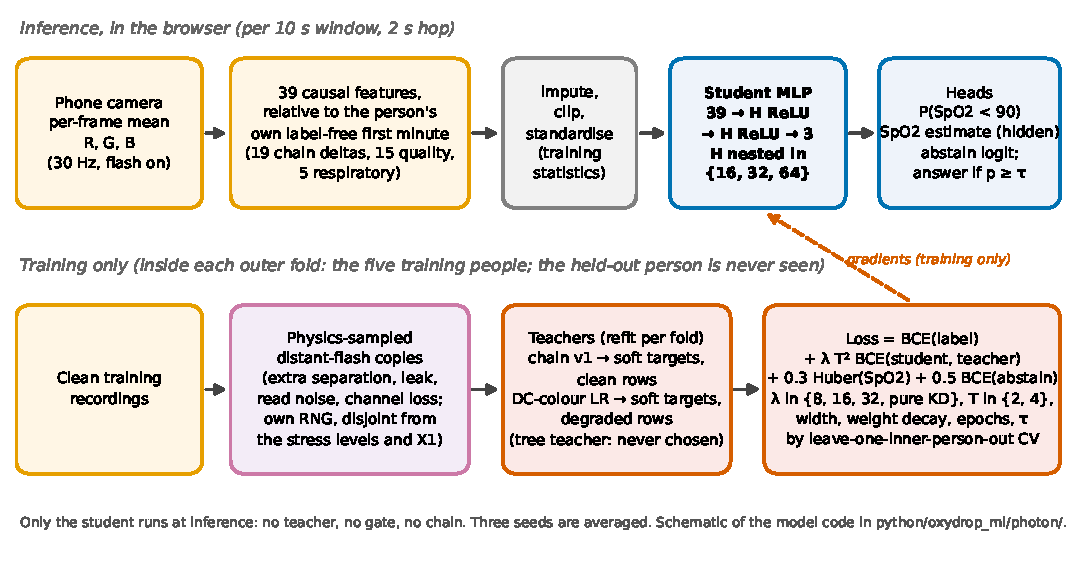
\includegraphics[width=0.95\linewidth]{figures/fig_arch.pdf}
\caption{PhotonDistill2. Top: inference in the browser. Bottom: training inside each fold. The teachers and the degraded copies exist only during training.}\label{fig:arch}
\end{figure}

\paragraph{Input.} Every 2~s the app computes 39 causal features of the last 10~s of per-frame mean R, G and B, each relative to the person's own label-free first minute: 19 chain deltas (heart-rate rise, ratio-of-ratios, pulse shape, DC colour), 15 signal-quality features and 5 respiratory features. The front end is the one of PhotonDistill. Imputation values, clipping bounds and standardisation come from the training people of the fold.

\paragraph{Network.} A multilayer perceptron $39\to H\to H\to3$ with ReLU activations. The hidden width $H\in\{16,32,64\}$ is chosen by nested cross-validation (2,435 parameters per student at $H=32$, 6,915 at $H=64$); the three deployed students have $H=32,32,64$ and are averaged. The three heads output the hypoxia logit (the score, $P(\spo{}<90\%)$), an \spo{} estimate in standardised units that the app never shows, and an abstain logit that predicts whether the hypoxia head is right. The model answers when the abstain probability reaches a threshold $\tau$ chosen on inner out-of-fold windows (answered accuracy and balanced accuracy at least 0.90).

\paragraph{Training inside each outer fold.} Two teachers are refit on the fold's five training people: the chain gives soft targets on clean windows, and a DC-colour logistic regression (three baseline-relative ln DC values) gives soft targets on physics-sampled distant-flash copies of the training recordings. A second teacher family that averages each of these with a gradient-boosted tree model was also in the search and was never chosen. The augmentation prior draws the extra separation, light leak, read noise and channel loss from declared ranges (four copies per training recording) from an independent random stream whose (level, seed) pairs are disjoint from the stress levels, and never samples X1. The loss is
\begin{equation}
\begin{split}
\mathcal L={}&\mathrm{BCE}(y,z)+\lambda_{\mathrm{kd}}T^2\,\mathrm{BCE}\big(\sigma(z/T),\,p_{\mathrm{teacher}}^{(T)}\big)\\
&+0.3\,\mathrm{Huber}(\widehat{\mathrm{SpO}}_2)+0.5\,\mathrm{BCE}\big(a,\mathbf{1}[\text{hypoxia head correct}]\big),
\end{split}
\end{equation}
with class balancing, clean windows weighted 1 and degraded windows 0.25, trained with Adam \citep{kingma2015adam} (learning rate $3\times10^{-3}$, batch 512). Pure distillation drops the label term. Selection is two-stage and nested, by leave-one-inner-person-out cross-validation on the criterion $0.5\,\mathrm{TM}(\text{clean})+0.5\,\mathrm{mean\,TM}(\text{degraded copies})$: first the teacher family, $\lambda_{\mathrm{kd}}\in\{8,16,32,\text{pure}\}$, $T\in\{2,4\}$ and epochs $\{15,30\}$ at width 32; then the width and weight decay $\{10^{-4},10^{-2}\}$ for the stage-one winner. Over the 18 seed folds, $\lambda_{\mathrm{kd}}=16$ was chosen 7 times and 32 nine times, $T=2$ 11 times and $T=4$ 7 times, width 32 ten times and 64 seven times, and 30 epochs 15 times (\texttt{results/photon/distill2\_log.md}). The grid edge that PhotonDistill hit (8 in all 18 folds) is now inside the grid. The planned PhotonTwin physics teacher and OxySeq or OxyTrack teachers were not used (the saved outputs of the latter two are leave-one-person-out predictions, so using them as teachers would leak).

\paragraph{Deployment.} The deployed weights are three students refit on all six people with the modal nested recipe of each seed ($\lambda_{\mathrm{kd}}=16,32,32$; $T=2,2,4$; $H=32,32,64$; weight decay $10^{-4}$; 30 epochs; mean $\tau=0.916$). The deployed model has therefore seen every Hoffman person, and the reported numbers are those of the leave-one-person-out fold models, not of the deployed files.

\paragraph{In-browser runtime.} The feature extractor is ported to JavaScript (\texttt{app/js/distill\_\allowbreak features.js}) and agrees with the Python extractor to $10^{-12}$ on fixture recordings. A small network runtime (\texttt{app/js/nn\_\allowbreak runtime.js}) executes plain operations (linear, 1D convolution, GRU, layer norm or folded batch norm, activations, pooling) from a JSON weight file in double precision and agrees with PyTorch to $4\times10^{-15}$ on its test network. The weights of PhotonDistill2 use the same file format as the round-2 engine, so the same app export script converts them without code changes, and the exported application forward pass reproduces the reference scores of two fixture windows to $2.4\times10^{-9}$. The app shows the model's output and abstention as they are, with fixed wording for the three states (Normal vs your baseline; Possible low oxygen, re-check with a pulse oximeter; Unsure, re-measure). Latency on phones was not measured for this paper. Nothing leaves the device.
\else
\TODO{The locked round-3 winner is \WinName{} (key \WinKey). Replace this subsection by its input, network, training, deployment and runtime description.}
\fi


\section{Results}\label{sec:results}

All numbers in this section are read from \texttt{results/photon/TABLE.csv} (written by \texttt{python -m oxydrop\_ml.photon.evalkit} from the score files). Intervals are 95\% person-bootstrap intervals over six people. The chain reads \ChainLzero{} \ChainLzeroCI{} on clean light. Stress levels are simulations.

\subsection{Clean light}
Table~\ref{tab:clean} and Figure~\ref{fig:forest} give the clean-light comparison. The shipped model scores \WinLzero{} \WinLzeroCI{}. Its paired difference to the chain is \WinLzeroDiff{} \WinLzeroDiffCI{}, verdict \emph{\WinLzeroVerdict}, with \WinLzeroBetter{} people better and a worst person at \WinLzeroWorst{} (chain: \ChainLzeroWorst{}). Over three seeds the mean is \WinSeedMeanLzero{} (\WinSeedN{} seed files). Its null control has mean TM \WinNullMean{} over \WinNullDraws{} draws (maximum \WinNullMax{}).

\begin{table}[t]
\centering
\caption{Clean light (L0), leave-one-person-out, six held-out people. TM: time-matched balanced accuracy of the forced decision. Paired difference: model minus chain on the same resampled people. $^{*}$: null-control mean above 0.55. The null column gives the mean TM of the control and, in brackets, the number of draws.}\label{tab:clean}
% GENERATED by make_numbers.py (tab_clean)
{\footnotesize
\setlength{\tabcolsep}{4pt}
\begin{adjustbox}{max width=\linewidth}
\begin{tabular}{p{3.6cm}lllcccc}
\toprule
Model & TM bal. acc. [95\% CI] & Paired diff. vs chain [95\% CI] & Verdict & People better & Worst person & Null mean (draws) & AUROC \\
\midrule
\multicolumn{8}{l}{\emph{Baselines}} \\
Logistic chain v1 & 0.796 [0.636, 0.857] & reference &  &  & 0.458 & -- & 0.947 \\
Logistic chain v1, C by nested CV & 0.786 [0.596, 0.860] & $-$0.010 [$-$0.082, $+$0.028] & tie & 3/6 & 0.463 & -- & 0.930 \\
Hybrid (chain + CNN), nested & 0.779 [0.638, 0.831] & $-$0.017 [$-$0.103, $+$0.069] & tie & 2/5 & 0.517 & -- & 0.891 \\
CNN alone (OxyNet, 3 seeds) & 0.753 [0.573, 0.817] & $-$0.043 [$-$0.140, $+$0.005] & tie & 2/6 & 0.500 & -- & 0.883 \\
\multicolumn{8}{l}{\emph{Controls (no network)}} \\
Control: DC-colour LR (3 values) & 0.744 [0.543, 0.848] & $-$0.052 [$-$0.155, $+$0.043] & tie & 2/6 & 0.514 & 0.500 (1) & 0.874 \\
Control: DC colour + AC optics LR & 0.701 [0.545, 0.782] & $-$0.096 [$-$0.197, $-$0.011] & loss & 2/6 & 0.500 & 0.500 (1) & 0.813 \\
Control: DC colour + dHR LR & 0.694 [0.546, 0.793] & $-$0.102 [$-$0.165, $-$0.016] & loss & 2/6 & 0.526 & 0.500 (1) & 0.878 \\
\multicolumn{8}{l}{\emph{Round 1 (designed before any score)}} \\
PhotonTwin-Inverse & 0.752 [0.577, 0.810] & $-$0.044 [$-$0.127, 0.000] & loss & 2/6 & 0.500 & 0.406 (1) & 0.904 \\
PhotonTwin-Inverse, physics path only & 0.693 [0.550, 0.759] & $-$0.103 [$-$0.226, $-$0.010] & loss & 2/6 & 0.500 & 0.455 (3) & 0.859 \\
FlashGap & 0.740 [0.607, 0.831] & $-$0.057 [$-$0.127, $+$0.021] & tie & 1/4 & 0.458 & 0.522 (2) & 0.899 \\
OxyTrack & 0.809 [0.656, 0.893] & $+$0.013 [$-$0.052, $+$0.092] & tie & 3/6 & 0.500 & -- & 0.912 \\
PhotonTwin gate (hand-coded, post hoc) & 0.796 [0.636, 0.857] & 0.000 [0.000, 0.000] & tie & 0/0 & 0.458 & 0.584 (3)$^{*}$ & 0.947 \\
FlashGap gate (post hoc) & 0.740 [0.606, 0.839] & $-$0.057 [$-$0.115, $+$0.014] & tie & 0/3 & 0.458 & 0.508 (2) & 0.933 \\
\multicolumn{8}{l}{\emph{Round 2 (trained end to end)}} \\
PhotonDistill & 0.758 [0.603, 0.813] & $-$0.038 [$-$0.103, $-$0.001] & loss & 2/6 & 0.516 & 0.492 (3) & 0.944 \\
OxySeq & 0.708 [0.452, 0.790] & $-$0.088 [$-$0.221, $-$0.023] & loss & 2/6 & 0.516 & 0.475 (1) & 0.877 \\
PhotonNet & 0.668 [0.508, 0.785] & $-$0.128 [$-$0.208, $-$0.047] & loss & 2/6 & 0.500 & 0.618 (3)$^{*}$ & 0.865 \\
OxySSL & 0.667 [0.498, 0.741] & $-$0.130 [$-$0.274, $-$0.044] & loss & 1/6 & 0.400 & 0.643 (3)$^{*}$ & 0.735 \\
\multicolumn{8}{l}{\emph{Round 3 (scaled up)}} \\
\textbf{PhotonDistill2} (shipped) & 0.784 [0.596, 0.834] & $-$0.012 [$-$0.091, $+$0.012] & tie & 4/6 & 0.500 & 0.504 (3) & 0.948 \\
PhotonDistill2, GPU rerun (seed variance) & 0.761 [0.561, 0.830] & $-$0.035 [$-$0.127, $-$0.006] & loss & 3/6 & 0.480 & 0.508 (3) & 0.944 \\
MultiDA & 0.744 [0.553, 0.807] & $-$0.053 [$-$0.142, $-$0.010] & loss & 3/6 & 0.500 & 0.522 (3) & 0.925 \\
PhotonNet-XL & 0.660 [0.545, 0.762] & $-$0.136 [$-$0.210, $-$0.033] & loss & 2/6 & 0.500 & 0.412 (3) & 0.865 \\
Ens-3 & 0.789 [0.621, 0.842] & $-$0.007 [$-$0.092, $+$0.043] & tie & 4/6 & 0.585 & -- & 0.938 \\
\bottomrule
\end{tabular}
\end{adjustbox}
}

\end{table}

\begin{figure}[t]
\centering
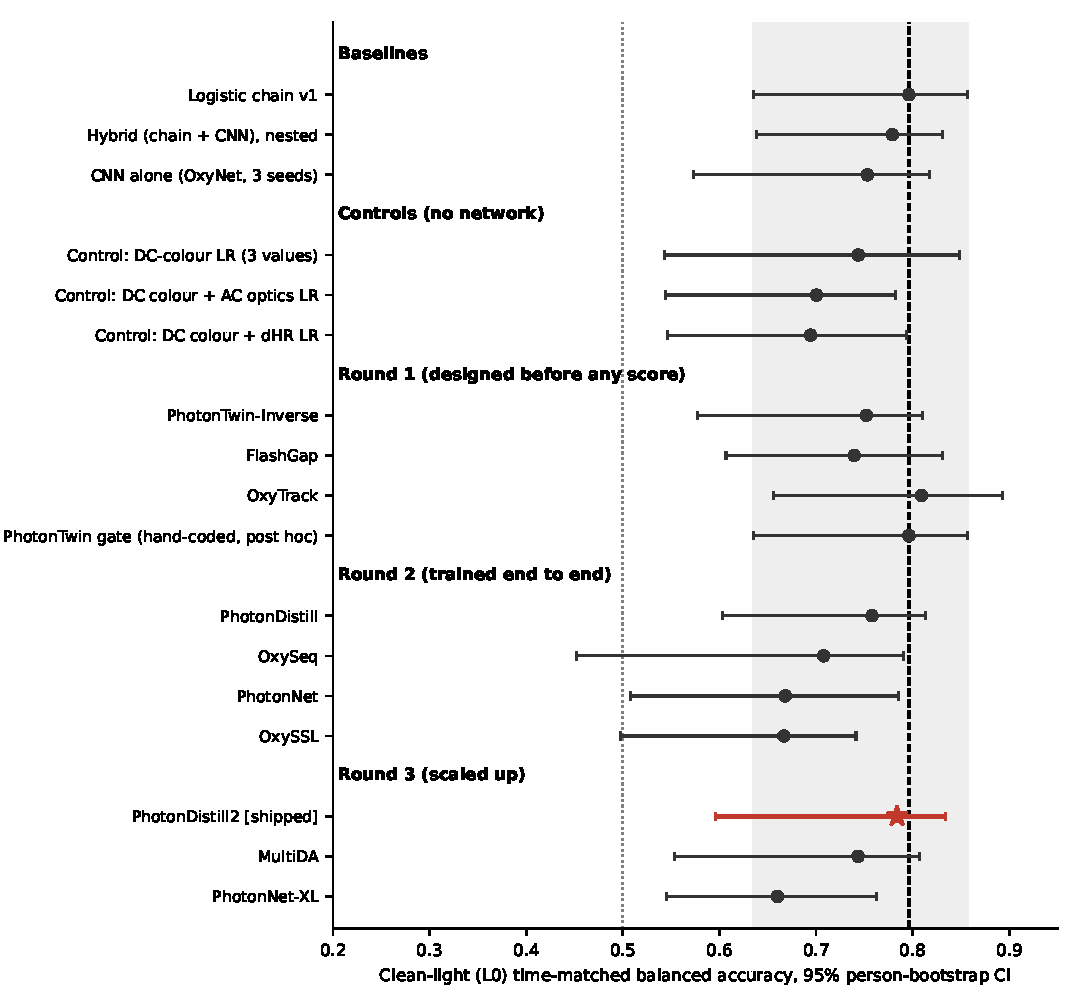
\includegraphics[width=0.85\linewidth]{figures/fig_forest.pdf}
\caption{Clean-light TM with 95\% person-bootstrap intervals. The dashed line is the chain, the grey band its interval, the dotted line chance. Models from rounds 2 and 3 were designed after earlier outer results were seen, so their clean-light numbers are optimistic.}\label{fig:forest}
\end{figure}

\subsection{Clean and simulated distant-flash light side by side}
Table~\ref{tab:stress} and Figure~\ref{fig:stress} show clean light (L0), three simulated levels and the out-of-family X1. The chain falls to \ChainLthree{} at L3 and \ChainXone{} at X1 and keeps answering at about chance (answered-window accuracy \ChainXoneAnsAcc{} at X1 with coverage \ChainXoneCov{}). The shipped model scores \WinLthree{}, \WinLfour{}, \WinLfive{} and \WinXone{} at L3, L4, L5 and X1, with paired differences to the chain of \WinLthreeDiff{} (\WinLthreeVerdict), \WinLfourDiff{} (\WinLfourVerdict), \WinLfiveDiff{} (\WinLfiveVerdict) and \WinXoneDiff{} (\WinXoneVerdict). Its mean paired difference over these four conditions is \WinStressMeanDiff{}, and the paired interval excludes 0 in \WinStressWins{} of the four. Table~\ref{tab:paired} lists all paired differences, with the number of people better.

\begin{table}[t]
\centering
\caption{TM balanced accuracy with 95\% person-bootstrap interval by condition. L3 to L5 are simulated distant-flash levels (Table~\ref{tab:stressdef}); X1 is out of family. Models are not refit per level.}\label{tab:stress}
% GENERATED by make_numbers.py (tab_stress)
{\scriptsize
\setlength{\tabcolsep}{2.5pt}
\begin{adjustbox}{max width=\linewidth}
\begin{tabular}{p{3.4cm}lllll}
\toprule
Model & L0 clean & L3 & L4 & L5 & X1 (out of family) \\
\midrule
\multicolumn{6}{l}{\emph{Baselines}} \\
Logistic chain v1 & 0.796 [0.636, 0.857] & 0.565 [0.503, 0.625] & 0.598 [0.526, 0.640] & 0.535 [0.477, 0.598] & 0.508 [0.439, 0.554] \\
Logistic chain v1, C by nested CV & 0.786 [0.596, 0.860] & 0.541 [0.476, 0.606] & 0.579 [0.518, 0.615] & 0.518 [0.467, 0.574] & 0.493 [0.424, 0.539] \\
Hybrid (chain + CNN), nested & 0.779 [0.638, 0.831] & n/a & n/a & n/a & n/a \\
CNN alone (OxyNet, 3 seeds) & 0.753 [0.573, 0.817] & n/a & n/a & n/a & n/a \\
\multicolumn{6}{l}{\emph{Controls (no network)}} \\
Control: DC-colour LR (3 values) & 0.744 [0.543, 0.848] & 0.692 [0.529, 0.769] & 0.658 [0.511, 0.748] & 0.599 [0.536, 0.652] & 0.646 [0.511, 0.735] \\
Control: DC colour + AC optics LR & 0.701 [0.545, 0.782] & 0.694 [0.596, 0.759] & 0.639 [0.581, 0.687] & 0.566 [0.502, 0.638] & 0.643 [0.560, 0.701] \\
Control: DC colour + dHR LR & 0.694 [0.546, 0.793] & 0.613 [0.498, 0.722] & 0.615 [0.540, 0.666] & 0.590 [0.517, 0.684] & 0.580 [0.469, 0.665] \\
\multicolumn{6}{l}{\emph{Round 1 (designed before any score)}} \\
PhotonTwin-Inverse & 0.752 [0.577, 0.810] & 0.652 [0.524, 0.770] & 0.624 [0.550, 0.702] & 0.625 [0.537, 0.724] & 0.615 [0.530, 0.683] \\
PhotonTwin-Inverse, physics path only & 0.693 [0.550, 0.759] & 0.719 [0.561, 0.774] & 0.715 [0.621, 0.751] & 0.647 [0.561, 0.717] & 0.693 [0.608, 0.746] \\
FlashGap & 0.740 [0.607, 0.831] & 0.603 [0.490, 0.732] & 0.663 [0.548, 0.770] & 0.619 [0.533, 0.709] & 0.628 [0.503, 0.714] \\
OxyTrack & 0.809 [0.656, 0.893] & 0.594 [0.488, 0.675] & 0.613 [0.541, 0.686] & 0.502 [0.453, 0.570] & 0.552 [0.503, 0.613] \\
PhotonTwin gate (hand-coded, post hoc) & 0.796 [0.636, 0.857] & 0.677 [0.600, 0.752] & 0.715 [0.621, 0.751] & 0.647 [0.561, 0.717] & 0.514 [0.454, 0.557] \\
FlashGap gate (post hoc) & 0.740 [0.606, 0.839] & 0.608 [0.479, 0.732] & 0.650 [0.553, 0.741] & 0.653 [0.579, 0.724] & 0.616 [0.490, 0.708] \\
\multicolumn{6}{l}{\emph{Round 2 (trained end to end)}} \\
PhotonDistill & 0.758 [0.603, 0.813] & 0.680 [0.552, 0.772] & 0.681 [0.566, 0.772] & 0.701 [0.570, 0.770] & 0.676 [0.564, 0.747] \\
OxySeq & 0.708 [0.452, 0.790] & 0.533 [0.399, 0.620] & 0.503 [0.493, 0.515] & 0.498 [0.490, 0.505] & 0.508 [0.441, 0.587] \\
PhotonNet & 0.668 [0.508, 0.785] & 0.689 [0.526, 0.812] & 0.703 [0.516, 0.829] & 0.720 [0.564, 0.818] & 0.672 [0.537, 0.775] \\
OxySSL & 0.667 [0.498, 0.741] & 0.697 [0.596, 0.733] & 0.548 [0.503, 0.601] & 0.522 [0.500, 0.552] & 0.686 [0.567, 0.732] \\
\multicolumn{6}{l}{\emph{Round 3 (scaled up)}} \\
\textbf{PhotonDistill2} (shipped) & 0.784 [0.596, 0.834] & 0.698 [0.555, 0.789] & 0.695 [0.558, 0.785] & 0.704 [0.562, 0.779] & 0.682 [0.547, 0.748] \\
PhotonDistill2, GPU rerun (seed variance) & 0.761 [0.561, 0.830] & 0.693 [0.561, 0.784] & 0.692 [0.569, 0.781] & 0.700 [0.558, 0.777] & 0.685 [0.550, 0.747] \\
MultiDA & 0.744 [0.553, 0.807] & 0.680 [0.559, 0.780] & 0.691 [0.559, 0.782] & 0.696 [0.557, 0.764] & 0.678 [0.547, 0.791] \\
PhotonNet-XL & 0.660 [0.545, 0.762] & 0.680 [0.520, 0.772] & 0.684 [0.522, 0.794] & 0.704 [0.563, 0.796] & 0.691 [0.597, 0.746] \\
Ens-3 & 0.789 [0.621, 0.842] & 0.713 [0.540, 0.792] & 0.683 [0.573, 0.774] & 0.675 [0.588, 0.764] & 0.704 [0.589, 0.779] \\
\bottomrule
\end{tabular}
\end{adjustbox}
}

\end{table}

\begin{table}[t]
\centering
\caption{Paired difference to the chain at the same level [95\% interval], verdict, and people better of people compared. A win requires the interval to exclude 0; otherwise the result is a tie.}\label{tab:paired}
% GENERATED by make_numbers.py (tab_paired)
{\tiny
\setlength{\tabcolsep}{2pt}
\begin{adjustbox}{max width=\linewidth}
\begin{tabular}{p{3.0cm}lllll}
\toprule
Model & L0 & L3 & L4 & L5 & X1 \\
\midrule
\multicolumn{6}{l}{\emph{Baselines}} \\
Logistic chain v1, C by nested CV & $-$0.010 [$-$0.082, $+$0.028] tie 3/6 & $-$0.023 [$-$0.049, $-$0.007] loss 0/5 & $-$0.019 [$-$0.036, $+$0.002] tie 2/6 & $-$0.016 [$-$0.033, $-$0.002] loss 1/5 & $-$0.014 [$-$0.026, $-$0.002] loss 2/5 \\
Hybrid (chain + CNN), nested & $-$0.017 [$-$0.103, $+$0.069] tie 2/5 & n/a & n/a & n/a & n/a \\
CNN alone (OxyNet, 3 seeds) & $-$0.043 [$-$0.140, $+$0.005] tie 2/6 & n/a & n/a & n/a & n/a \\
\multicolumn{6}{l}{\emph{Controls (no network)}} \\
Control: DC-colour LR (3 values) & $-$0.052 [$-$0.155, $+$0.043] tie 2/6 & $+$0.127 [$-$0.015, $+$0.232] tie 4/6 & $+$0.060 [$-$0.051, $+$0.163] tie 5/6 & $+$0.064 [$-$0.026, $+$0.150] tie 4/6 & $+$0.139 [$-$0.014, $+$0.225] tie 5/5 \\
Control: DC colour + AC optics LR & $-$0.096 [$-$0.197, $-$0.011] loss 2/6 & $+$0.130 [$+$0.037, $+$0.188] win 3/6 & $+$0.041 [$+$0.005, $+$0.107] win 6/6 & $+$0.031 [$-$0.061, $+$0.114] tie 4/6 & $+$0.136 [$+$0.050, $+$0.222] win 6/6 \\
Control: DC colour + dHR LR & $-$0.102 [$-$0.165, $-$0.016] loss 2/6 & $+$0.049 [$-$0.033, $+$0.117] tie 5/5 & $+$0.017 [$-$0.003, $+$0.043] tie 6/6 & $+$0.056 [$+$0.004, $+$0.107] win 5/5 & $+$0.073 [$-$0.033, $+$0.192] tie 6/6 \\
\multicolumn{6}{l}{\emph{Round 1 (designed before any score)}} \\
PhotonTwin-Inverse & $-$0.044 [$-$0.127, 0.000] loss 2/6 & $+$0.087 [0.000, $+$0.170] win 4/6 & $+$0.026 [$-$0.020, $+$0.087] tie 4/6 & $+$0.090 [$+$0.020, $+$0.154] win 5/5 & $+$0.107 [$+$0.023, $+$0.213] win 6/6 \\
PhotonTwin-Inverse, physics path only & $-$0.103 [$-$0.226, $-$0.010] loss 2/6 & $+$0.154 [$+$0.016, $+$0.226] win 4/6 & $+$0.117 [$+$0.061, $+$0.178] win 6/6 & $+$0.112 [$+$0.022, $+$0.207] win 5/6 & $+$0.185 [$+$0.086, $+$0.264] win 6/6 \\
FlashGap & $-$0.057 [$-$0.127, $+$0.021] tie 1/4 & $+$0.038 [$-$0.037, $+$0.136] tie 3/4 & $+$0.065 [$-$0.018, $+$0.159] tie 5/5 & $+$0.085 [$+$0.013, $+$0.163] win 4/5 & $+$0.121 [0.000, $+$0.240] tie 4/5 \\
OxyTrack & $+$0.013 [$-$0.052, $+$0.092] tie 3/6 & $+$0.029 [$-$0.023, $+$0.070] tie 2/6 & $+$0.015 [$-$0.044, $+$0.082] tie 4/6 & $-$0.033 [$-$0.108, $+$0.034] tie 4/6 & $+$0.044 [$-$0.001, $+$0.104] tie 4/6 \\
PhotonTwin gate (hand-coded, post hoc) & 0.000 [0.000, 0.000] tie 0/0 & $+$0.112 [$+$0.052, $+$0.172] win 5/6 & $+$0.117 [$+$0.061, $+$0.178] win 6/6 & $+$0.112 [$+$0.022, $+$0.207] win 5/6 & $+$0.007 [0.000, $+$0.026] tie 1/1 \\
FlashGap gate (post hoc) & $-$0.057 [$-$0.115, $+$0.014] tie 0/3 & $+$0.043 [$-$0.045, $+$0.125] tie 4/5 & $+$0.052 [$-$0.017, $+$0.135] tie 6/6 & $+$0.118 [$+$0.059, $+$0.173] win 5/6 & $+$0.109 [$-$0.020, $+$0.228] tie 5/5 \\
\multicolumn{6}{l}{\emph{Round 2 (trained end to end)}} \\
PhotonDistill & $-$0.038 [$-$0.103, $-$0.001] loss 2/6 & $+$0.116 [$-$0.002, $+$0.226] tie 4/6 & $+$0.083 [$+$0.008, $+$0.178] win 6/6 & $+$0.166 [$+$0.035, $+$0.242] win 5/6 & $+$0.169 [$+$0.058, $+$0.285] win 6/6 \\
OxySeq & $-$0.088 [$-$0.221, $-$0.023] loss 2/6 & $-$0.032 [$-$0.133, $+$0.046] tie 3/6 & $-$0.094 [$-$0.137, $-$0.015] loss 3/6 & $-$0.036 [$-$0.098, $+$0.017] tie 2/6 & $+$0.001 [$-$0.047, $+$0.059] tie 3/6 \\
PhotonNet & $-$0.128 [$-$0.208, $-$0.047] loss 2/6 & $+$0.125 [$-$0.019, $+$0.267] tie 4/6 & $+$0.105 [$-$0.025, $+$0.245] tie 5/6 & $+$0.185 [$+$0.023, $+$0.290] win 5/6 & $+$0.165 [$+$0.020, $+$0.316] win 6/6 \\
OxySSL & $-$0.130 [$-$0.274, $-$0.044] loss 1/6 & $+$0.132 [$+$0.024, $+$0.171] win 1/6 & $-$0.050 [$-$0.123, $+$0.045] tie 3/6 & $-$0.013 [$-$0.098, $+$0.068] tie 2/5 & $+$0.178 [$+$0.043, $+$0.214] win 5/6 \\
\multicolumn{6}{l}{\emph{Round 3 (scaled up)}} \\
\textbf{PhotonDistill2} (shipped) & $-$0.012 [$-$0.091, $+$0.012] tie 4/6 & $+$0.133 [$+$0.001, $+$0.248] win 4/6 & $+$0.097 [$+$0.011, $+$0.195] win 6/6 & $+$0.170 [$+$0.027, $+$0.249] win 5/6 & $+$0.174 [$+$0.044, $+$0.284] win 6/6 \\
PhotonDistill2, GPU rerun (seed variance) & $-$0.035 [$-$0.127, $-$0.006] loss 3/6 & $+$0.129 [$+$0.007, $+$0.245] win 4/6 & $+$0.094 [$+$0.018, $+$0.190] win 6/6 & $+$0.166 [$+$0.022, $+$0.247] win 5/6 & $+$0.177 [$+$0.044, $+$0.287] win 6/6 \\
MultiDA & $-$0.053 [$-$0.142, $-$0.010] loss 3/6 & $+$0.115 [$+$0.003, $+$0.216] win 4/6 & $+$0.093 [$+$0.002, $+$0.189] win 6/6 & $+$0.161 [$+$0.026, $+$0.232] win 5/6 & $+$0.170 [$+$0.027, $+$0.328] win 6/6 \\
PhotonNet-XL & $-$0.136 [$-$0.210, $-$0.033] loss 2/6 & $+$0.115 [$-$0.028, $+$0.229] tie 3/6 & $+$0.086 [$-$0.020, $+$0.207] tie 5/6 & $+$0.169 [$+$0.018, $+$0.270] win 5/6 & $+$0.184 [$+$0.072, $+$0.290] win 6/6 \\
Ens-3 & $-$0.007 [$-$0.092, $+$0.043] tie 4/6 & $+$0.149 [$-$0.007, $+$0.255] tie 4/6 & $+$0.085 [$+$0.003, $+$0.193] win 6/6 & $+$0.141 [$+$0.043, $+$0.248] win 5/6 & $+$0.197 [$+$0.074, $+$0.280] win 6/6 \\
\bottomrule
\end{tabular}
\end{adjustbox}
}

\end{table}

\begin{figure}[t]
\centering
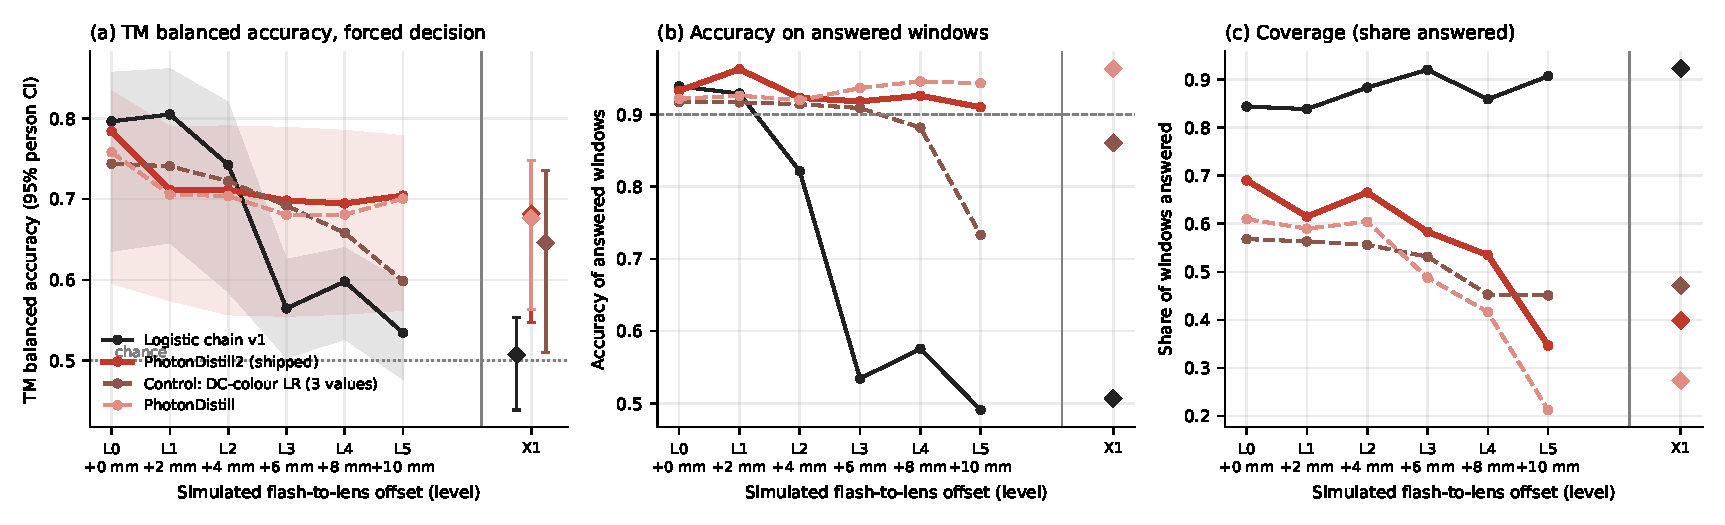
\includegraphics[width=\linewidth]{figures/fig_stress.pdf}
\caption{Simulated distant-flash stress. (a) TM balanced accuracy of the forced decision (bands: 95\% person-bootstrap interval; diamonds: out-of-family X1). (b) Accuracy of the windows the model chooses to answer. (c) Share of windows answered. Only the held-out person is degraded. Levels are simulations, not measurements of a phone.}\label{fig:stress}
\end{figure}

\begin{table}[t]
\centering
\caption{Own abstention: coverage / accuracy on answered windows. Random abstention at the same coverage keeps the all-window accuracy in expectation, so answered accuracy is informative only when it exceeds that.}\label{tab:abstain}
% GENERATED by make_numbers.py (tab_abstain)
{\footnotesize
\setlength{\tabcolsep}{4pt}
\begin{adjustbox}{max width=\linewidth}
\begin{tabular}{p{3.8cm}lllll}
\toprule
Model & L0 & L3 & L4 & L5 & X1 \\
\midrule
Logistic chain v1 & 0.84 / 0.939 & 0.92 / 0.534 & 0.86 / 0.576 & 0.91 / 0.491 & 0.92 / 0.507 \\
\textbf{PhotonDistill2} (shipped) & 0.69 / 0.933 & 0.58 / 0.918 & 0.53 / 0.926 & 0.35 / 0.910 & 0.40 / 0.861 \\
Control: DC-colour LR (3 values) & 0.57 / 0.917 & 0.53 / 0.909 & 0.45 / 0.882 & 0.45 / 0.733 & 0.47 / 0.861 \\
PhotonDistill & 0.61 / 0.922 & 0.49 / 0.937 & 0.42 / 0.946 & 0.21 / 0.943 & 0.27 / 0.964 \\
OxySeq & 0.79 / 0.769 & 0.71 / 0.556 & 0.71 / 0.543 & 0.71 / 0.539 & 0.71 / 0.583 \\
\bottomrule
\end{tabular}
\end{adjustbox}
}

\end{table}

\subsection{Round-3 candidates}
Against the chain on clean light, PhotonDistill2 (shipped) scores \DistillTwoLzero{} (paired \DistillTwoLzeroDiff{} \DistillTwoLzeroDiffCI{}, \DistillTwoLzeroVerdict), MultiDA \MultidaLzero{} (\MultidaLzeroDiff{} \MultidaLzeroDiffCI{}, \MultidaLzeroVerdict) and PhotonNet-XL \PhotonnetXlLzero{} (\PhotonnetXlLzeroDiff{} \PhotonnetXlLzeroDiffCI{}, \PhotonnetXlLzeroVerdict). Under stress all three beat or tie the chain; at X1 they score \DistillTwoXone{}, \MultidaXone{} and \PhotonnetXlXone{}. Scale did not help PhotonNet-XL: an encoder about three times larger (15.4 k against 4.9 k inference parameters) lands at the clean-light level of round-2 PhotonNet. Adding MTHS and BUT PPG rows (MultiDA) changed little: its Hoffman-only ablation scores \MultidaHofonlyLzero{} against \MultidaLzero{}, well inside the intervals. \ifHasEnsThree Ens3: \EnsThreeLzero{} \EnsThreeLzeroCI{} (\EnsThreeLzeroVerdict). \else Ens3 and SSL3 are not scored here (Section~\ref{sec:candidates}). \fi The GPU rerun of PhotonDistill2 (\DistillTwoGpuLzero{}, paired \DistillTwoGpuLzeroDiff{} \DistillTwoGpuLzeroDiffCI{}) is listed in Table~\ref{tab:full} and discussed in Section~\ref{sec:discussion} as seed variance.

\subsection{Abstention}
Table~\ref{tab:abstain} gives coverage and answered accuracy. The chain keeps answering when the signal is gone, and its answered accuracy falls to chance. A model with a learned abstain output can lower its coverage as the light weakens (Figure~\ref{fig:stress}c). The OxySeq abstain head did not notice the low light in round 2. The shipped model answers \WinLzeroCov{} of windows on clean light with answered accuracy \WinLzeroAnsAcc{}, and \WinXoneCov{} at X1 with \WinXoneAnsAcc{}. Answered accuracy is compared with the all-window accuracy in \texttt{SIDE\_BY\_SIDE.md} before it is called a gain.

\subsection{Per-person results and the colour control}
Table~\ref{tab:person} shows the six people at L0. The chain's per-person TM is highest for P1 and lowest for P2 (the only dark-skinned participant), whose score is \ChainLzeroWorst{}. The three-number DC-colour control scores \DcLrLzero{} \DcLrLzeroCI{} at L0 (paired \DcLrLzeroDiff{} \DcLrLzeroDiffCI{}, \DcLrLzeroVerdict), \DcLrLfour{} at L4 and \DcLrXone{} at X1 (paired \DcLrXoneDiff{} \DcLrXoneDiffCI{}, \DcLrXoneVerdict). Its paired difference to the physics-only path of PhotonTwin-Inverse includes 0 at L0 to L4 and X1 (\texttt{controls\_log.md}).

\begin{table}[t]
\centering
\caption{Per-person TM at L0 (P1 to P6 are the six held-out people).}\label{tab:person}
% GENERATED by make_numbers.py (tab_person)
{\footnotesize
\setlength{\tabcolsep}{4pt}
\begin{adjustbox}{max width=\linewidth}
\begin{tabular}{p{4cm}cccccc}
\toprule
Model & P1 & P2 & P3 & P4 & P5 & P6 \\
\midrule
Logistic chain v1 & 0.889 & 0.458 & 0.660 & 0.711 & 0.737 & 0.539 \\
\textbf{PhotonDistill2} (shipped) & 0.673 & 0.500 & 0.666 & 0.714 & 0.718 & 0.551 \\
Control: DC-colour LR (3 values) & 0.659 & 0.514 & 0.626 & 0.625 & 0.693 & 0.869 \\
PhotonDistill & 0.670 & 0.516 & 0.649 & 0.721 & 0.700 & 0.536 \\
\bottomrule
\end{tabular}
\end{adjustbox}
}

\end{table}

\subsection{Ablations}
Table~\ref{tab:ablate} lists ablations and earlier versions of each trained model, scored on the same harness. Ablations are not eligible to be promoted.

\begin{table}[t]
\centering
\caption{Ablations and variants (clean-light TM [interval], paired difference to the chain, X1 and L4 TM).}\label{tab:ablate}
% GENERATED by make_numbers.py (tab_ablate)
{\footnotesize
\setlength{\tabcolsep}{4pt}
\begin{adjustbox}{max width=\linewidth}
\begin{tabular}{p{4.2cm}lllc}
\toprule
Variant & L0 TM [95\% CI] & Paired diff. vs chain & X1 TM & L4 TM \\
\midrule
PhotonDistill & 0.758 [0.603, 0.813] & $-$0.038 [$-$0.103, $-$0.001] & 0.676 & 0.681 \\
PhotonDistill, no teachers & 0.660 [0.529, 0.760] & $-$0.136 [$-$0.216, $-$0.038] & 0.626 & 0.654 \\
PhotonDistill v1 (before post hoc grid) & 0.696 [0.524, 0.795] & $-$0.100 [$-$0.201, $-$0.022] & 0.658 & 0.667 \\
\addlinespace
OxySeq & 0.708 [0.452, 0.790] & $-$0.088 [$-$0.221, $-$0.023] & 0.508 & 0.503 \\
OxySeq, no test-time adaptation & 0.639 [0.437, 0.764] & $-$0.158 [$-$0.265, $-$0.058] & 0.513 & 0.446 \\
\addlinespace
PhotonNet & 0.668 [0.508, 0.785] & $-$0.128 [$-$0.208, $-$0.047] & 0.672 & 0.703 \\
PhotonNet, no physics layer & 0.642 [0.528, 0.749] & $-$0.154 [$-$0.218, $-$0.061] & 0.663 & 0.657 \\
\addlinespace
OxySSL & 0.667 [0.498, 0.741] & $-$0.130 [$-$0.274, $-$0.044] & 0.686 & 0.548 \\
OxySSL, init only & 0.506 [0.410, 0.581] & $-$0.290 [$-$0.397, $-$0.156] & 0.524 & 0.500 \\
OxySSL, no augmentation & 0.652 [0.455, 0.779] & $-$0.144 [$-$0.327, $-$0.011] & 0.672 & 0.502 \\
\addlinespace
MultiDA & 0.744 [0.553, 0.807] & $-$0.053 [$-$0.142, $-$0.010] & 0.678 & 0.691 \\
MultiDA, Hoffman rows only & 0.730 [0.549, 0.804] & $-$0.066 [$-$0.151, $-$0.018] & 0.666 & 0.692 \\
\addlinespace
\bottomrule
\end{tabular}
\end{adjustbox}
}

\end{table}

\subsection{Null controls}
Table~\ref{tab:nulls} lists every null and blank control on the harness. A mean above 0.55 fails. Two round-2 models (PhotonNet and OxySSL) fail, so their stress wins are not usable. The chain itself, refit on \ChainNullN{} label permutations, has mean \ChainNullMean{} and SD \ChainNullSD{}, so a single draw above 0.55 is ordinary for a chain-like model and a single draw at 0.50 is weak evidence.

\begin{table}[t]
\centering
\caption{Null controls at L0 (labels permuted globally across training windows; blank = blank observations). Mean TM over draws.}\label{tab:nulls}
% GENERATED by make_numbers.py (tab_nulls)
{\footnotesize
\setlength{\tabcolsep}{4pt}
\begin{adjustbox}{max width=\linewidth}
\begin{tabular}{p{4.4cm}lcccl}
\toprule
Model & Control & Draws & Mean TM & Max TM & Rule (mean $\le$ 0.55) \\
\midrule
Control: DC-colour LR (3 values) & null & 1 & 0.500 & 0.500 & ok \\
Control: DC colour + AC optics LR & null & 1 & 0.500 & 0.500 & ok \\
Control: DC colour + dHR LR & null & 1 & 0.500 & 0.500 & ok \\
PhotonTwin-Inverse & null & 1 & 0.406 & 0.406 & ok \\
PhotonTwin-Inverse, physics path only & null & 3 & 0.455 & 0.523 & ok \\
FlashGap & null & 2 & 0.522 & 0.549 & ok \\
OxyTrack & blank & 1 & 0.500 & 0.500 & ok \\
PhotonTwin gate (hand-coded, post hoc) & null & 3 & 0.584 & 0.623 & NOT PASSED \\
FlashGap gate (post hoc) & null & 2 & 0.508 & 0.551 & ok \\
PhotonDistill & null & 3 & 0.492 & 0.560 & ok \\
OxySeq & null & 1 & 0.475 & 0.475 & ok \\
OxySeq & blank & 1 & 0.500 & 0.500 & ok \\
PhotonNet & null & 3 & 0.618 & 0.624 & NOT PASSED \\
OxySSL & null & 3 & 0.643 & 0.660 & NOT PASSED \\
\textbf{PhotonDistill2} (shipped) & null & 3 & 0.504 & 0.543 & ok \\
MultiDA & null & 3 & 0.522 & 0.541 & ok \\
PhotonNet-XL & null & 3 & 0.412 & 0.445 & ok \\
\bottomrule
\end{tabular}
\end{adjustbox}
}

\end{table}

\section{Discussion}\label{sec:discussion}

\paragraph{The clean-light result.}
\ifWinLossLzero
The shipped trained model \emph{loses} to the logistic chain on clean light: \WinLzero{} against \ChainLzero{}, paired \WinLzeroDiff{} \WinLzeroDiffCI{}, with \WinLzeroBetter{} people better. The upper end of the interval is close to 0, so the evidence for a real deficit is weak, but it cannot be called a tie by our pre-stated rule. It was shipped because the project required a genuinely trained end-to-end model with in-browser inference, which ruled out the chain and the hand-coded gates as the headline, and because it had the highest clean-light point estimate among eligible trained models with passed nulls.
\fi
\ifWinTieLzero
The shipped trained model is \emph{on par with} the logistic chain on clean light (a tie by our pre-stated rule): \WinLzero{} against \ChainLzero{}, paired \WinLzeroDiff{} \WinLzeroDiffCI{}, with \WinLzeroBetter{} people better and a worst person at \WinLzeroWorst{} (chain: \ChainLzeroWorst{}). A tie is not equality. The point estimate is below the chain's, the interval is wide with six people, and the model does not meet the criteria for beating the chain (a paired interval above 0 and at least 5 of 6 people better). Its predecessor in round 2 was a \DistillLzeroVerdict{} (\DistillLzero{}, paired \DistillLzeroDiff{} \DistillLzeroDiffCI{}). The paired improvement of the shipped model over that predecessor is \WinVsDistillLzero{} \WinVsDistillLzeroCI{}, which is itself not resolved from zero. The gain came from a wider and nested search of the distillation weight, temperature and width, not from new teachers (the gradient-boosted teacher was never chosen).
\fi
\ifWinWinLzero
The shipped trained model beats the logistic chain on clean light by the pre-stated paired criterion: \WinLzero{} against \ChainLzero{}, paired \WinLzeroDiff{} \WinLzeroDiffCI{}, with \WinLzeroBetter{} people better. This is a third look at the same six people by a model designed after earlier outer results were seen, so it is not a blind confirmation.
\fi

\paragraph{Seed variance: the locked run and the GPU rerun.}
The locked run (CPU) scored \WinLzero{} \WinLzeroCI{} on clean light. After the lock we reran the same code with the student network on a Kaggle T4 GPU (\texttt{results/photon/distill2\_gpu\_log.md}; same teachers, grid, seeds, batch order and initial weights). That rerun scored \DistillTwoGpuLzero{} \DistillTwoGpuLzeroCI{}, paired to the chain \DistillTwoGpuLzeroDiff{} \DistillTwoGpuLzeroDiffCI{}, with \DistillTwoGpuLzeroBetter{} people better and a worst person at \DistillTwoGpuLzeroWorst{}. We report the difference as seed variance: GPU and CPU float32 sums accumulate in a different order, which over up to 30 epochs of Adam changed which grid point won the inner search in 5 of 18 seed folds (the other 13 match, with slightly different trained weights). The two scores are two draws of the same method on six people. The locked run is on par with the chain; the rerun is slightly below it, with a paired interval that lies just below 0; neither beats the chain. At X1 the runs agree (\DistillTwoGpuXone{} on the GPU against \WinXone{}). The GPU weights were not swapped into the app, and every other number in this paper for the shipped model is the locked run's.
The shipped model was also locked after the cutoff of the round-3 timeline (Section~\ref{sec:candidates}), a decision made after its scores were seen. Two further reasons keep clean light from being decisive. Six people give wide intervals, and the clean-light numbers of all trained models come from designs made after the outer-fold scores were seen.

\paragraph{Robustness under the simulated distant flash.}
The chain collapses toward chance under simulated stress while the shipped model keeps most of its accuracy (Table~\ref{tab:stress}). That the simulated levels sit inside the augmentation prior of the shipped model and the teachers means L1 to L5 are in-simulator. X1 is the only level that tests more than the simulator family, and the shipped model scores \WinXone{} there against \ChainXone{} for the chain (paired \WinXoneDiff{} \WinXoneDiffCI{}). This is evidence about simulated degradation and says nothing about a real iPhone with a distant flash.

\paragraph{The DC-colour control is nearly as robust.}
A logistic regression on three baseline-relative ln DC values, with no network, scores \DcLrXone{} at X1 against \WinXone{} for the shipped model, and its paired interval to the chain includes 0 at X1 (\DcLrXoneDiffCI{}). Features relative to the person's own first minute cancel a constant multiplicative attenuation by construction, so part of any model's stress robustness is built into the feature definition. The same cue is the reason the network can be robust, and the stress simulation is mostly a constant attenuation plus an additive non-pulsatile leak. A real phone with different gain control or colour processing could break that cancellation for the control and for every model that uses it. In round 2, the same student without teachers scores \DistillNoKdLzero{} on clean light against \DistillLzero{} with them (Table~\ref{tab:ablate}), so the distillation matters for clean light even if the colour cue carries the stress robustness.

\paragraph{Designs made after results were seen.}
All of round 2 and round 3 were designed after the round-1 outer results on the same six people were seen, using cues (heart rate, DC colour, baseline-relative inputs) that had been identified on all six. PhotonDistill (round 2) was tuned after its first version's outer result (v1: \DistillVoneLzero{}) was seen, and its largest distillation weight was chosen in every fold. The grid of PhotonDistill2 was widened because of that edge hit, which is a design made after outer results were seen. Within the wider grid all choices are nested, and the optimum is bracketed (values 16 and 32 were chosen most often; pure distillation was never chosen). Round-1 gates were designed after outer results. OxyTrack's clean-light result (0.809) is optimistic because four versions were scored on outer folds. A selection effect among round-3 candidates by their clean-light point estimate adds a further, unquantified bias. These steps are listed in Section~\ref{sec:chronology}.

\paragraph{Sample and generalisation.}
There are six people, one of whom is dark-skinned, recorded with one phone model (Nexus 6P) at rest under induced desaturation. Intervals are wide, ``tie'' mostly means ``cannot distinguish'', and one person drives much of the chain's clean-light result. We make no skin-tone claim. The windows of one person are strongly dependent, and the effective sample for the paired comparison is six. No real distant-flash phone, other Android phone or iPhone has been measured. The chain is not a perfect reference baseline either, because its regularisation was fixed before the harness existed (Amendment 1 discloses a mild selection on evaluation people).

\section{Limitations}\label{sec:limits}
\begin{itemize}
\item \textbf{Data.} Six people, 12 recordings, one phone, rest only. No exercise, arrhythmia or beta-blocker data in the test set. In the project's earlier exercise false-alarm test on normoxic people, 63.4\% of exercise windows were flagged (the raw extraction is not reproducible here), so exercise is a known failure mode of heart-rate-based cues.
\item \textbf{Simulation.} The stress levels are a model of a distant flash with a design-chosen path scale. Real devices will differ.
\item \textbf{Label.} The label is the window-mean reference oximeter reading. The reference is a pulse oximeter, not arterial blood.
\item \textbf{Starting state.} The method measures a drop from the person's own baseline and cannot tell whether the person was already low during the first minute.
\item \textbf{TM.} TM scores only the desaturation transitions (bins with both classes). It does not measure performance on long stable segments.
\item \textbf{Abstention.} Answered accuracy depends on which windows the model skips; conformal-style abstention can skip exactly the transition windows that TM rewards.
\item \textbf{Licences.} Weights trained on restricted data (MTHS: CC BY-NC-ND; OpenOximetry: PhysioNet agreement) are shared for non-commercial research use under the project owner's decision, without confirmation from the data owners.
\end{itemize}

\section{Ethics, safety and health disclaimer}\label{sec:ethics}
\textbf{This is a research prototype and not a medical device.} It does not measure \spo{} and does not diagnose. A result of ``Normal vs your baseline'' is never reassurance, because the model measures a change from the person's own first minute and cannot detect that they were already low. A possible-low result is a prompt to re-check with a pulse oximeter or seek care, not a diagnosis. No one should delay care or replace a pulse oximeter or a clinician with this app. It has not been validated on any phone, and it has not been validated for any skin tone.

All human data come from public or credentialed datasets collected by others under their own consent procedures; we collected none. The app does not store or upload user data: frames are averaged in the browser and discarded. The main risks are false reassurance, uneven performance across skin tones and devices (pulse-oximeter bias is documented \citep{sjoding2020,fawzy2022}), and over-reading six people. We report the weakest person and the one dark-skinned person's result instead of hiding them, publish only aggregates for restricted data, and state the licence terms of derived weights. Any clinical use would need prospective validation across skin pigmentation, phones and saturation ranges, in line with regulatory guidance \citep{fda2025}.

\section{Reproducibility}\label{sec:repro}
Code, score files, pre-registration and its eight amendments are in the repository, branch \texttt{\RepoBranch}, commit \texttt{\RepoCommit}\ifRepoDirty{} (working tree had uncommitted result files when this text was generated; regenerate after the final commit)\fi. Every number in this paper is read from \texttt{results/photon/TABLE.csv} by \texttt{paper/make\_numbers.py}.
\begin{verbatim}
cd python && python -m oxydrop_ml.photon.evalkit   # TABLE.csv, STRESS.csv
python -m oxydrop_ml.photon.winner2                # WINNER2.md
python -m oxydrop_ml.photon.winner3                # WINNER3.md
python paper/make_numbers.py --winner KEY --locked # numbers.tex, tables/
python paper/make_figures.py                       # figures/fig_*.pdf
cd paper && tectonic oxydrop_photon.tex            # see paper/README.md
npm test                                           # JS parity of the engine
\end{verbatim}
Training of the heavy models ran on cloud sandboxes (scripts \texttt{scripts/ml\_daytona.py}); checkpoints stay outside git, and score files plus weights of the shipped model are in \texttt{results/photon/}. OpenOximetry-derived arrays never leave the credentialed analysis hosts.

\section*{Acknowledgments}
Built for the Veritas AI International High School Hackathon 2026, Health track. We thank the authors of the Hoffman, MTHS, BUT PPG and OpenOximetry datasets and the Oregon Medical Laser Center for the tissue-optics tables.

\bibliographystyle{plainnat}
\bibliography{refs}

\appendix

\section{Chronology of looks at the outer folds}\label{sec:chronology}
Times are U.S. Central, November 15, 2026, from the planner's log (\texttt{task.json}). Each row states what had been seen when a later design was made. This is the record that qualifies every clean-light number above.
\begin{description}
\item[16:58] FlashGap score files existed before the Amendment 6 draft was written (about 17:00); the preparation agent saw one FlashGap point in a regenerated figure.
\item[17:15] The planner read round-1 outer results and asked for an SNR-gated FlashGap variant. It is post hoc.
\item[17:37] After seeing twin\_inverse outer results, the planner asked for the PhotonTwin gate (chain when red SNR is at least 10 dB, else the physics path; threshold fixed a priori). It is post hoc.
\item[17:48] Four OxyTrack versions were scored on outer folds during development (0.673, 0.774, 0.815, 0.809), so its clean-light result is optimistic.
\item[17:50] DC-colour controls showed the physics path's robustness is mostly the baseline-relative DC colour cue.
\item[18:05] Round-1 decision: no candidate beats the chain on clean light; the PhotonTwin gate was shipped, then demoted.
\item[18:23] Round 2 started: the shipped model must be a trained end-to-end network, with no gate. Amendment 7 and its rule were written at about 18:28, before any round-2 score.
\item[19:13 to 19:32] Round-2 results. PhotonDistill v2 was tuned after its v1 outer result. The rule had no branch for ``no model ties the chain''; the extension was written after the results.
\item[19:50 to 19:55] Round 3 started with a cloud compute plan and a replacement rule (Amendment 8, written before any round-3 score). Candidates launched at 19:57.
\item[20:08 to 20:17] PhotonDistill2 clean-light ensemble (20:08, development), then its final clean-light, null and stress files (20:16, one minute after the 20:15 cutoff). MultiDA and PhotonNet-XL landed at 20:17.
\item[20:18] \texttt{winner3.py}: PhotonDistill2 passes the numeric rule but is late, so the script reports no replacement.
\item[20:22] Lock: the planner chooses PhotonDistill2 as the round-3 winner and records the lateness.
\item[20:25] Ens3 score files land after the lock, without null controls. SSL3 produced none.
\item[21:28 to 21:45] Score and null files of the GPU rerun of PhotonDistill2 arrive, after the lock. They are reported as seed variance and do not change the shipped model.
\end{description}

\section{All models and variants}\label{sec:fulltable}
Table~\ref{tab:full} lists every model and variant on the harness (no seeds or nulls). TM balanced accuracy at L0 with interval, paired verdict to the chain, and TM at L3 to L5 and X1.

% GENERATED by make_numbers.py (tab_full)
{\scriptsize\setlength{\tabcolsep}{3pt}
\begin{longtable}{@{}p{3.4cm}p{3.3cm}p{2.7cm}cccc@{}}
\caption{All models and variants on the harness (key as in \texttt{TABLE.csv}; paired verdict to the chain at L0; TM at the other conditions).}\label{tab:full}\\
\toprule
Model key & L0 TM [95\% CI] & vs chain & L3 & L4 & L5 & X1 \\
\midrule
\endfirsthead
\toprule
Model key & L0 TM [95\% CI] & vs chain & L3 & L4 & L5 & X1 \\
\midrule
\endhead
\bottomrule
\endfoot
\texttt{chain\_v1} & 0.796 [0.636, 0.857] &  reference & 0.565 & 0.598 & 0.535 & 0.508 \\
\texttt{chain\_v1\_nestedC} & 0.786 [0.596, 0.860] & $-$0.010 tie & 0.541 & 0.579 & 0.518 & 0.493 \\
\texttt{hybrid\_final} & 0.779 [0.638, 0.831] & $-$0.017 tie & n/a & n/a & n/a & n/a \\
\texttt{cnn\_full} & 0.753 [0.573, 0.817] & $-$0.043 tie & n/a & n/a & n/a & n/a \\
\texttt{ctl\_dc\_lr} & 0.744 [0.543, 0.848] & $-$0.052 tie & 0.692 & 0.658 & 0.599 & 0.646 \\
\texttt{ctl\_dc\_ror\_lr} & 0.701 [0.545, 0.782] & $-$0.096 loss & 0.694 & 0.639 & 0.566 & 0.643 \\
\texttt{ctl\_dc\_hr\_lr} & 0.694 [0.546, 0.793] & $-$0.102 loss & 0.613 & 0.615 & 0.590 & 0.580 \\
\texttt{twin\_inverse} & 0.752 [0.577, 0.810] & $-$0.044 loss & 0.652 & 0.624 & 0.625 & 0.615 \\
\texttt{twin\_inverse\_noresid} & 0.693 [0.550, 0.759] & $-$0.103 loss & 0.719 & 0.715 & 0.647 & 0.693 \\
\texttt{flashgap} & 0.740 [0.607, 0.831] & $-$0.057 tie & 0.603 & 0.663 & 0.619 & 0.628 \\
\texttt{oxytrack} & 0.809 [0.656, 0.893] & $+$0.013 tie & 0.594 & 0.613 & 0.502 & 0.552 \\
\texttt{twin\_gate} & 0.796 [0.636, 0.857] & 0.000 tie & 0.677 & 0.715 & 0.647 & 0.514 \\
\texttt{flashgap\_gate} & 0.740 [0.606, 0.839] & $-$0.057 tie & 0.608 & 0.650 & 0.653 & 0.616 \\
\texttt{distill} & 0.758 [0.603, 0.813] & $-$0.038 loss & 0.680 & 0.681 & 0.701 & 0.676 \\
\texttt{oxyseq} & 0.708 [0.452, 0.790] & $-$0.088 loss & 0.533 & 0.503 & 0.498 & 0.508 \\
\texttt{photonnet} & 0.668 [0.508, 0.785] & $-$0.128 loss & 0.689 & 0.703 & 0.720 & 0.672 \\
\texttt{oxyssl} & 0.667 [0.498, 0.741] & $-$0.130 loss & 0.697 & 0.548 & 0.522 & 0.686 \\
\texttt{distill2} & 0.784 [0.596, 0.834] & $-$0.012 tie & 0.698 & 0.695 & 0.704 & 0.682 \\
\texttt{multida} & 0.744 [0.553, 0.807] & $-$0.053 loss & 0.680 & 0.691 & 0.696 & 0.678 \\
\texttt{photonnet\_xl} & 0.660 [0.545, 0.762] & $-$0.136 loss & 0.680 & 0.684 & 0.704 & 0.691 \\
\texttt{distill\_nokd} & 0.660 [0.529, 0.760] & $-$0.136 loss & 0.633 & 0.654 & 0.705 & 0.626 \\
\texttt{distill\_v1} & 0.696 [0.524, 0.795] & $-$0.100 loss & 0.650 & 0.667 & 0.706 & 0.658 \\
\texttt{distill\_v1\_nokd} & 0.670 [0.548, 0.769] & $-$0.126 loss & 0.624 & 0.653 & 0.695 & 0.615 \\
\texttt{flashgap\_noaug} & 0.787 [0.650, 0.865] & $-$0.009 tie & 0.550 & 0.587 & 0.551 & 0.506 \\
\texttt{flashgap\_nosnr} & 0.756 [0.560, 0.848] & $-$0.040 tie & 0.533 & 0.565 & 0.521 & 0.492 \\
\texttt{flashgap\_v1} & 0.675 [0.571, 0.786] & $-$0.121 loss & 0.664 & 0.675 & 0.642 & 0.641 \\
\texttt{flashgap\_v2} & 0.748 [0.604, 0.853] & $-$0.048 tie & 0.648 & 0.714 & 0.706 & 0.632 \\
\texttt{multida\_hofonly} & 0.730 [0.549, 0.804] & $-$0.066 loss & 0.652 & 0.692 & 0.703 & 0.666 \\
\texttt{oxyseq\_notta} & 0.639 [0.437, 0.764] & $-$0.158 loss & 0.558 & 0.446 & 0.468 & 0.513 \\
\texttt{oxyssl\_init} & 0.506 [0.410, 0.581] & $-$0.290 loss & 0.540 & 0.500 & 0.500 & 0.524 \\
\texttt{oxyssl\_noaug} & 0.652 [0.455, 0.779] & $-$0.144 loss & 0.701 & 0.502 & 0.500 & 0.672 \\
\texttt{oxytrack\_ema} & 0.798 [0.635, 0.850] & $+$0.002 tie & 0.567 & 0.604 & 0.533 & 0.510 \\
\texttt{oxytrack\_noadapt} & 0.819 [0.659, 0.901] & $+$0.022 tie & 0.556 & 0.563 & 0.484 & 0.510 \\
\texttt{oxytrack\_nosnr} & 0.840 [0.692, 0.906] & $+$0.043 tie & 0.609 & 0.638 & 0.560 & 0.550 \\
\texttt{photonnet\_nophys} & 0.642 [0.528, 0.749] & $-$0.154 loss & 0.650 & 0.657 & 0.662 & 0.663 \\
\texttt{twin\_chain} & 0.781 [0.627, 0.845] & $-$0.015 tie & 0.570 & 0.601 & 0.541 & 0.512 \\
\texttt{twin\_chain\_nestedC} & 0.754 [0.598, 0.814] & $-$0.042 tie & 0.549 & 0.591 & 0.544 & 0.498 \\
\texttt{twin\_gate\_soft} & 0.788 [0.617, 0.842] & $-$0.009 loss & 0.679 & 0.720 & 0.646 & 0.527 \\
\texttt{twin\_inverse\_v1} & 0.736 [0.544, 0.844] & $-$0.060 tie & 0.585 & 0.546 & 0.514 & 0.531 \\
\end{longtable}
}


\end{document}
